%TEXT FROM:
%http://www.newadvent.org/bible/1ma001.htm

\documentclass[10pt]{book} % use larger type; default would be 10pt

\usepackage[latin1]{luainputenc}

\usepackage[oldstyle]{libertine}
\usepackage{lettrine}
\usepackage{xcolor}

% dual language parallel text thing
\usepackage{eledmac}
\usepackage{eledpar}

% BLUES
\definecolor{benblue1}{HTML}{2B22C7}

% REDS
\definecolor{benred8}{HTML}{E82C00} %seems good, maybe the best?

% THREE COMMANDS TO CLEAN UP ALL THE ELEDPAR/ELEDMAC STUFF
\newcommand{\StartOfLatin}{
	\begin{pairs}
	\begin{Leftside}
	\firstlinenum{10000}\linenumincrement{10000}\beginnumbering\pstart
}

\newcommand{\StartOfEnglish}{
	\pend\endnumbering
	\end{Leftside}
	\begin{Rightside}

	\firstlinenum{10000}\linenumincrement{10000}\beginnumbering\pstart
}

\newcommand{\EndOfEnglish}{
	\pend\endnumbering
	\end{Rightside}
	\end{pairs}
	\Columns
}

\usepackage{fancyhdr}
\pagestyle{fancy}
\cfoot{\textcolor{benblue1}{\thepage}}
\renewcommand{\headrulewidth}{0pt}

%redefine 'plain' page styel to have blue page numbers too
\fancypagestyle{plain}{
	\chead{}
	\cfoot{\textcolor{benblue1}{\thepage}}

}

\begin{document}

\chapter*{Ezekiel}

\begin{large}\begin{center}\textsc{Chapter i}\end{center}\end{large}
\lettrine[lines=3]{T}{hirty} years had passed;\footnote[1]{This must refer either to the prophet\textquotesingle s age, or to some date artificially chosen, e.g. the rediscovery of the Law under Josias.} it was the fifth day of the fourth month, and I was sharing the lot of the exiles by the river Chobar, when heaven opened, and I saw a vision of God. \textcolor{benred8}{2}~The fifth day of the month, and the fifth year since king Joachin was banished. \textcolor{benred8}{3}~To the priest Ezechiel, son of Buzi, the divine word came; there in the Chaldaean land, by the river Chobar, the power of the Lord could reach him.
\textcolor{benred8}{4}~I looked round me, to find that a storm-wind had sprung up from the north, driving a great cloud before it; and this cloud had fire caught up in it, that fringed it with radiance. And there in the heart of it, in the very heart of the fire, was a glow like amber, \textcolor{benred8}{5}~that enclosed four living figures. These were human in appearance, \textcolor{benred8}{6}~but each had four faces, and two pairs of wings. \textcolor{benred8}{7}~Either leg was straight-formed, yet ended in a calf\textquotesingle s hoof; they sparkled like red-hot bronze. \textcolor{benred8}{8}~On each of the four sides, human arms shewed beneath the wings; faces and wings looked outwards four ways.\footnote[2]{It is not easy to form a clear picture of what the prophet saw; but it seems most probable that the four figures stood back to back in a square, the eight upper wings all touching. If so, the \textasciigrave four sides\textquotesingle  will be the four sides of the square, and each angel will have had one arm (or hand) shewing underneath either of his lower wings.} \textcolor{benred8}{9}~Wings of each were held touching wings of other; and when they moved, they did not turn round, but each kept an onward course. \textcolor{benred8}{10}~As for the appearance of their faces, each had the face of a man, yet each of the four looked like a lion when seen from the right, like an ox when seen from the left, like an eagle when seen from above.\footnote[3]{If the assumption made in the previous note is true, we can understand why no reference is made to the appearance of the angelic body from behind; we are given a view from above instead. But the Hebrew text and the other versions omit the word \textasciigrave above\textquotesingle , leaving the whole picture in considerable confusion.} \textcolor{benred8}{11}~So much for their faces; each had two wings spread out above him, those two which met his neighbours\textquotesingle  wings; with the other two he veiled his body. \textcolor{benred8}{12}~Each of them marched straight forward, following the movement of a divine impulse, never swerving as he marched. \textcolor{benred8}{13}~There was that, too, in the appearance of the living figures which put me in mind of flaming coals, or of torches; that was what I saw going to and fro in the midst of the living figures, a glow as of fire, and from this glow lightning came out. \textcolor{benred8}{14}~So the living creatures came and went, vivid as lightning-flashes.
\textcolor{benred8}{15}~And as I watched the living figures, all at once wheels appeared close to them, one at each of the four sides, \textcolor{benred8}{16}~of strange colour and form. All four were alike, the colour of aquamarine,\footnote[4]{Literally, \textasciigrave a vision of the sea\textquotesingle . The Latin translators seem to have supposed, here as in Is. 23.10 and elsewhere, that \textasciigrave Tharsis\textquotesingle  was a Hebrew word meaning \textasciigrave sea\textquotesingle . (In 10.9 the rendering given is \textasciigrave chrysolith\textquotesingle ). Here, as in Ex. 28.20, it evidently means some kind of precious stone, possibly jasper. It is doubtful whether the phrase \textasciigrave a wheel within a wheel\textquotesingle  describes a wheel with an inner circle joining its spokes in addition to the outside rim, or to two wheels intersecting one another at right angles, forming a kind of approach to a sphere.} and each looked like a wheel within a wheel. \textcolor{benred8}{17}~Moved they, it was ever one of the four ways the living figures looked; and they did not turn round in moving. \textcolor{benred8}{18}~As for their size, their height was terrible to look upon; and the whole frame of them, all round, was full of eyes. \textcolor{benred8}{19}~Onward the wheels moved, when the living figures moved onward, at their side; rose above the earth when the living figures rose above it. \textcolor{benred8}{20}~They too had a living impulse in them, they too, whenever that impulse stirred them, must rise up and follow the way it went; \textcolor{benred8}{21}~with the living figures, whose vital impulse they shared, the wheels too moved, and halted, and rose.
\textcolor{benred8}{22}~Over the living figures a vault seemed to rise, like a sheet of dazzling crystal resting on their heads; \textcolor{benred8}{23}~under this vault each held two wings erect to meet his neighbour\textquotesingle s. Each had two turned upwards to overshadow him, and two turned downwards to veil his body.\footnote[5]{The Hebrew text of this verse is perhaps corrupt; it seems to imply that each angel used all four wings to veil his body, which is in contradiction with all the other evidence this chapter provides. The statement in the Latin version that \textasciigrave each of them veiled his body with two wings, and the other one was veiled similarly\textquotesingle  yields no acceptable sense.} \textcolor{benred8}{24}~When they moved, the sound of their wings reached me, loud as waters in flood or thunders from on high,\footnote[6]{Literally, \textasciigrave the voice of the most High\textquotesingle ; it seems clear that thunder is referred to, cf. Apoc. 14.2.} incessant as the hum of a great throng or an armed camp; only when they came to rest did they lower their wings. \textcolor{benred8}{25}~A voice would come from the firmament over their heads; then they would halt, then they would lower their wings.\footnote[7]{This is the sense given in the Latin version to a sentence in the Hebrew which is obscure, and perhaps corrupt.} \textcolor{benred8}{26}~Above this vault that rested on them, sapphire blue towered up into the form of a throne, nor did that throne seem to be empty; a shape was there above it, as of one enthroned, \textcolor{benred8}{27}~and all about him it was filled with amber-coloured flame. Upwards from his loins, downwards from his loins, an arch of light seemed to shine, \textcolor{benred8}{28}~like rainbow among the clouds on a day of storm; there was brightness all about him.
\begin{large}\begin{center}\textsc{Chapter ii}\end{center}\end{large}
\lettrine[lines=2]{S}{o} much I saw of what the Lord\textquotesingle s glory is like; and seeing it, I fell down face to earth. And now I heard a voice, which said to me, Rise up, son of man, I must have speech with thee. \textcolor{benred8}{2}~And at his words, a divine force mastered me, raising me to my feet, so that I could listen to him. \textcolor{benred8}{3}~Son of man, he told me, I am sending thee on an errand to the men of Israel, this heathen brood that has rebelled and forsaken me; see how my covenant has been violated by the fathers yesterday, the children to-day! \textcolor{benred8}{4}~To brazen-faced folk and hard-hearted thy errand is, and still from the Lord God a message thou must deliver, \textcolor{benred8}{5}~hear they or deny thee hearing; rebels all, at least they shall know that they have had a prophet in their midst. \textcolor{benred8}{6}~Never fear them, son of man, never let rebuke of theirs dishearten thee; with the unbelieving and the unruly\footnote[1]{The Hebrew text is generally interpreted as meaning \textasciigrave thorns and briers\textquotesingle .} thou must learn to live, scorpions ever at thy side; rebels all, they must not frighten thee, must not dishearten thee. \textcolor{benred8}{7}~Hear they or deny thee hearing, remonstrate with them thou must; they are a defiant brood.
\textcolor{benred8}{8}~Do my bidding, then, son of man; no rebel thou, like those others; open thy mouth and eat what I give thee. \textcolor{benred8}{9}~And with that, I saw a hand stretched out towards me, with a closed book in it; and this, when he opened it to my view, had writing on both sides of it; nothing was there but dirge and lamenting, nothing but cries of woe.
\begin{large}\begin{center}\textsc{Chapter iii}\end{center}\end{large}
\lettrine[lines=2]{S}{on} of man, he told me, eat thou must what eat thou canst; here is this scroll for thy eating. After that, go and give my message to the sons of Israel. \textcolor{benred8}{2}~Thereupon I opened my mouth, and he gave me the scroll to eat, \textcolor{benred8}{3}~promising me safe digestion and a full belly with the gift; and indeed, it was sweet as honey when I ate it. \textcolor{benred8}{4}~Now, son of man, said he, to the men of Israel betake thee, and give them my message. \textcolor{benred8}{5}~Are they strange folk that lisp and stammer,\footnote[1]{Literally, \textasciigrave of deep speech and unknown tongue\textquotesingle ; in the Hebrew text, \textasciigrave of deep lips and heavy tongue\textquotesingle . The language of the other Semitic races suggested an attempt to talk Hebrew under difficulties.} these men of Israel? Ah, no; \textcolor{benred8}{6}~nations there are a many that lisp and stammer, past thy understanding, but I am sending thee to Israel instead. These might have listened to thee;\footnote[2]{Literally, in the Latin, \textasciigrave If I were sending thee to these, they would be listening to thee\textquotesingle . The sense of the Hebrew text is probably, \textasciigrave But no, I am sending thee to these (the Israelites). These (the other nations) would be listening to thee\textquotesingle .} \textcolor{benred8}{7}~hearing from Israel thou shalt have none; my word goes ever unheeded, so stubborn of forehead they are and so hard-hearted, all the brood of them. \textcolor{benred8}{8}~But see, I have given thee strength of brow, hardness of forehead, that shall outmatch theirs; \textcolor{benred8}{9}~unyielding as flint or adamant thou shalt face them. Fear them not, never let their frown daunt thee, this brood of rebels.
\textcolor{benred8}{10}~Then he said to me, Son of man, all the words I tell thee heed and hear; \textcolor{benred8}{11}~then to captive Israel betake thee, and give them thy message in the name of the Lord God, hear they or deny thee hearing. \textcolor{benred8}{12}~And with that, a sudden transport seized me, and as I went, I heard the noise of a great stir behind me.~\ldots\  Blessed be the glory of the Lord~\ldots\  from the place where he was.\footnote[3]{If one consonant is altered, the Hebrew text would give the sense, \textasciigrave I heard the noise of a great stir behind me, as the glory of the Lord rose up from the place where it was\textquotesingle .} \textcolor{benred8}{13}~Beat of wing against wing as the living figures moved onwards, and whirr of the wheels that followed them, great stirring there was all about me; \textcolor{benred8}{14}~and I, in a transport borne up and on, set out on my journey, unwillingly enough, and vexed at heart, but the Lord\textquotesingle s hand was there to hold me to my purpose. \textcolor{benred8}{15}~So I made my way to the settlement of exiles at Tel-Abib,\footnote[4]{Tel-Abib (not the modern Tel-Aviv, in Palestine) is translated, instead of being transliterated, in the Latin version; \textasciigrave to the Mound of New Crops\textquotesingle .} near the river Chobar; and when I had found them, I sat there for seven days in their company, dumb all the while with grief.
\textcolor{benred8}{16}~Then, when seven days had passed, the Lord\textquotesingle s word came to me. \textcolor{benred8}{17}~Son of man, he told me, I am posting thee here as a sentry, to give the sons of Israel warning; no message I send thee but thou must pass it on in my name. \textcolor{benred8}{18}~When I threaten I the sinner with doom of death, it is for thee to give him word, and warn him, as he loves his life, to have done with sinning. If not, he shall die as he deserves, but for his undoing thyself shalt be called to account. \textcolor{benred8}{19}~If thou warn him, and leave his rebellious sinning he will not, die he shall as he deserves, and thou go free. \textcolor{benred8}{20}~Or if the upright man leaves his innocence, and I take him unawares in his wrong-doing, dies he for want of warning? Die he shall, his good deeds all forgotten, but thou for his undoing shalt be called to account. \textcolor{benred8}{21}~Thine to warn the upright man against the marring of his innocence; and he, sin avoiding, shall owe his life to thy remonstrance; thy duty is done.\footnote[5]{vv. 16-21. The sense of these verses, and in great part the actual language of them, can be found repeated in ch. 33, and some think they have been misplaced here through an error.}
\textcolor{benred8}{22}~Then the power of the Lord came over me, bidding me rise up and keep tryst with him, out in the open plain. \textcolor{benred8}{23}~Rise up I did, and when I reached the open plain, there was the glory of the Lord rising above it, such as I had seen it by the banks of Chobar; and I fell face to earth. \textcolor{benred8}{24}~But a divine force mastered me and raised me to my feet again. Now go within doors, he said, and shut thyself in there~\ldots\  \textcolor{benred8}{25}~And thou, son of man~\ldots\  here are bonds confining thee; closely thy fellow-countrymen shall keep thee imprisoned, so that thou canst not escape from them. \textcolor{benred8}{26}~And I, meanwhile, will keep tongue of thine fast fixed in thy mouth; dumb thou shalt be, when thou wouldst fain expostulate with a rebellious brood. \textcolor{benred8}{27}~Then, when my message I give thee, I will unseal thy lips, and thou shalt speak to that rebellious brood in the name of the Lord God, hear they or deny thee hearing.\footnote[6]{vv. 24-27. There has perhaps been some fault in the manuscript transmission of these verses, which run very awkwardly. The Hebrew text has \textasciigrave so that thou canst not go out among them\textquotesingle  instead of \textasciigrave so that thou canst not escape from them\textquotesingle .}
\begin{large}\begin{center}\textsc{Chapter iv}\end{center}\end{large}
\lettrine[lines=2]{A}{nd} now, son of man, go and get thee a tile; set it before thee and make marks on it, to represent the city of Jerusalem. \textcolor{benred8}{2}~This thou art to beleaguer; siege-works built, mound raised, camp pitched, battering-rams all around.\footnote[1]{vv. 1, 2. It is not clear whether the prophet was to draw a map, or simply to write the name, of Jerusalem. The directions in verse 2 may be simply an anticipation of verse 3; the rim of the iron cooking-vessel was to represent the continuous cordon of besiegers.} \textcolor{benred8}{3}~And therewithal get thee an iron cooking-pan, that shall make a ring of iron between thee and this city of thine; look closely as thou wilt, here is siege complete. So thou shalt beleaguer it; a sign, this, for the race of Israel.
\textcolor{benred8}{4}~This, too, thou must do; ever on thy left side lie down to sleep, weighing it down, day after day as thou sleepest upon it, with the guilt of Israel; bear it thou must. \textcolor{benred8}{5}~Three hundred and ninety days of guilt-bearing I have allotted thee, one day for every year of Israel\textquotesingle s guilt; \textcolor{benred8}{6}~this done, Juda\textquotesingle s guilt thou must bear for forty days yet, sleeping on thy right side; a day for a year, for every year a day. \textcolor{benred8}{7}~And ever towards beleaguered Jerusalem thou shalt turn thy face, and hold thy arm stretched out, prophesying its doom; \textcolor{benred8}{8}~I hold thee enchained, and never shalt thou turn from one side to other, till the days of thy siege are over.\footnote[2]{vv. 4-8. The word rendered \textasciigrave to sleep\textquotesingle  in the Latin may also mean \textasciigrave to lie\textquotesingle , and it is generally understood that the prophet was to remain all day and all night in the same posture. The figures are extremely perplexing. We should have expected that the days would be equal in number with those of the siege, but this, according to IV Kg. 25, lasted about 500 days. The forty years do not match the interval between the taking of Samaria in 722 and the taking of Jerusalem in 587. And we should expect the other figure to correspond with the number of years between the division of the Kingdom and the fall of Samaria, i.e. about 410 years; instead of which the Hebrew text gives 390 and the Septuagint Greek 190.}
\textcolor{benred8}{9}~For thy food, wheat thou must have by thee, and barley, and beans, and lentils, and spelt, and vetch; all in one pan mix them, and make thee bread, while thou art sleeping ever on thy same side; for three hundred and ninety days thou shalt eat it.\footnote[3]{The different kinds of crop are probably meant to symbolize the simultaneous deficiency of all bread-stuffs; cf. verse 16.} \textcolor{benred8}{10}~Nine ounces shall be all thy daily food, at set times apportioned, \textcolor{benred8}{11}~and water thou shalt drink at set times, two pints by measure. \textcolor{benred8}{12}~Cooked in the ashes thy bread, like barley cakes, and dung of man shall be thy fuel, for all to see. \textcolor{benred8}{13}~Polluted as this, the Lord says, shall be the bread Israel eats, in the land I have decreed for his exile.
\textcolor{benred8}{14}~Alas, alas, Lord God, said I, here is a soul that never knew defilement; from childhood\textquotesingle s days, beast I never ate that died by chance or lay mangled, nor ever did food unclean cross my lips. \textcolor{benred8}{15}~Be it so, he answered; for dung of man droppings of cattle thou shalt have, and cook thy bread with these. \textcolor{benred8}{16}~But be sure of this, son of man; I mean to cut off from Jerusalem every source of bread; weighed out to them their bread shall be, and anxiously, measured out to them their water, and in great lack. \textcolor{benred8}{17}~And at last, for want of bread and water, every man\textquotesingle s face shall fall as he looks at other, and they shall pine away in their guilt.
\begin{large}\begin{center}\textsc{Chapter v}\end{center}\end{large}
\lettrine[lines=2]{A}{nd} next, son of man, to the sharp sword betake thee! A razor thou must take, and pass it over head and beard both; then weigh thy hair in the scales and make equal portions of it. \textcolor{benred8}{2}~A third of it thou shalt set alight and burn up within this city of thine, when the days of its besieging are over; a third thou shalt cut to pieces with the blade thou carriest, round about it; and a third thou shalt scatter to the winds, for my unsheathed sword to go in pursuit. \textcolor{benred8}{3}~Of this last third, gather some few hairs and secure them in the fold of thy cloak; \textcolor{benred8}{4}~yet even of these take some away and throw them into the heart of the fire, to burn there; fire enough to kindle the whole race of Israel!\footnote[1]{It is not clear what is meant by the last clause of this verse.}
\textcolor{benred8}{5}~Look you, says the Lord God, here is Jerusalem, that I have set down at earth\textquotesingle s very midst, the nations all about her, \textcolor{benred8}{6}~and she has defied my will, than the very heathen more rebellious, defied my commandments, as neighbouring peoples never did. My bidding they have cast to the winds, followed never where my commandments led. \textcolor{benred8}{7}~All your neighbours, the Lord God says, outdone in wickedness, my paths untrodden, my bidding unheeded! False even to the heathen traditions of yonder country-side! \textcolor{benred8}{8}~Have at thee, says the Lord God; in thy very heart I will execute judgement for all the world to see; \textcolor{benred8}{9}~such punishment I will inflict as never was before, never shall be again, for thy detestable doings. \textcolor{benred8}{10}~Men\textquotesingle s flesh men shall eat, father of son and son of father; then, when my sentence is executed, I will scatter all that is left of thee to the four winds.
\textcolor{benred8}{11}~As I am a living God, the Lord says, since thou hast not scrupled to profane my sanctuary with vile things and detestable things a many, I will make havoc of thee, and my eye shall not melt with pity; I will not scruple in my turn. \textcolor{benred8}{12}~A third of thy sons shall die of pestilence, or with famine pine away; a third shall fall in thy defence; a third I will scatter to the four winds, and my sword unsheathed in pursuit. \textcolor{benred8}{13}~And at last, my anger spent, my vengeance glutted, my grief healed, doubt they shall not that the God whom they slighted has decreed it; my sentence shall take full toll of them. \textcolor{benred8}{14}~Desolate, and the scorn of thy neighbours, so every passer-by shall see thee. \textcolor{benred8}{15}~A name of scorn and reproach, a by-word thou shalt be and a thing of horror, to all the nations about thee, when thy punishment is done, so fierce the anger, so shrewd the blow; \textcolor{benred8}{16}~I, the Lord, have decreed it. Hungry arrows\footnote[2]{Literally, \textasciigrave arrows of hunger\textquotesingle , but it seems likely that the other plagues about to be mentioned are included, as well as the famine.} of mine shall fly abroad, dolorous and deadly, for your minishing; famine that grows worse and worse as the stocks of bread fail, \textcolor{benred8}{17}~and with the famine wild beasts to bereave you, visitations of plague and violent death; and the sword too, I will let loose upon you; I, the Lord, have decreed it.
\begin{large}\begin{center}\textsc{Chapter vi}\end{center}\end{large}
\lettrine[lines=2]{A}{nd} now the Lord\textquotesingle s word came to me: \textcolor{benred8}{2}~Turn thy eyes, son of man, towards the hills of thy own country, and prophesy their doom. \textcolor{benred8}{3}~Mountains of Israel, thou shalt say, listen to the word of the Lord God; here is a message from the Lord God to mountain and hill, to rocky slope and river-bed. I mean to let the sword loose on you, pull shrine down, \textcolor{benred8}{4}~overthrow altar, break column, pile corpses before the false god\textquotesingle s feet; \textcolor{benred8}{5}~before every idol, sons of Israel prostrate in death, before every altar, the ground strewn with their bones. \textcolor{benred8}{6}~In all your confines, every city desolate, every shrine wrecked and ruined; deserted and defaced the altars, forlorn the idols, shattered the columns, obliterated all the work of man; \textcolor{benred8}{7}~and ever the dead lying in the midst of you. Will you doubt, then, the power of the Lord?\footnote[1]{vv. 6, 7. It is not clear whether we should take these verses as part of the first paragraph (addressed to the mountains) or as part of the second (addressed to the Israelites themselves).}
\textcolor{benred8}{8}~I will leave a remnant of you; some shall escape the sword, to live on among the Gentiles, dispersed far and wide; \textcolor{benred8}{9}~and these survivors, in their land of exile, shall once again bethink themselves of me. Wanton heart that played me false, eyes that hankered still after idols, shall be tamed now; they will look back with loathing on all the foul wrong they did, \textcolor{benred8}{10}~and confess it was no empty boast, when I threatened this calamity.\footnote[2]{vv. 8-10. These verses seem to interrupt the thread of the chapter, and some think they have been accidentally misplaced.}
\textcolor{benred8}{11}~Clap hands and stamp feet, the Lord God says, and cry aloud, Out upon the foul wrong the men of Israel did, that are now doomed to perish by sword, famine and pestilence! \textcolor{benred8}{12}~Keep they their distance, the plague shall smite them, come they to grips, the sword; safe behind the battlements, they shall die of famine; so shall my vengeance take toll of them. \textcolor{benred8}{13}~Who shall doubt the Lord\textquotesingle s power, when the dead lie thick at the feet of your idols and about your altars; on hill-top and mountain height, in forest covert and under spreading oak, where once men would burn fragrant incense to their false gods? \textcolor{benred8}{14}~When the blow falls, I will make their countryside, once so thickly inhabited, into a wilderness; Deblatha\footnote[3]{No such place as Deblatha is elsewhere heard of, and there may be some error in the text.} itself is not more forlorn. And who shall doubt the Lord\textquotesingle s power?
\begin{large}\begin{center}\textsc{Chapter vii}\end{center}\end{large}
\lettrine[lines=2]{T}{hen} the Lord\textquotesingle s word came to me: \textcolor{benred8}{2}~And thou, son of man~\ldots\ \footnote[1]{It seems probable that there is some slight omission in the manuscripts here.} A message to the land of Israel from the Lord God! For this land, for every corner of it, here is doom, here is doom. \textcolor{benred8}{3}~Doom for thee at last; I mean to wreak vengeance on thee, pass sentence on thy evil life, bring home to thee thy foul deeds. \textcolor{benred8}{4}~Nor shall my eye melt with pity; I will not spare. All thy evil life brought home to thee, all thy foul deeds confronting thee; who shall doubt that it comes from the Lord? \textcolor{benred8}{5}~The blow, the first blow has fallen, says the Lord God; \textcolor{benred8}{6}~all is over now, all is over; the day dawns, and for thee doom comes with day. \textcolor{benred8}{7}~Dwellers in the land, this is the end of you; your time is up, your day has come; a day when your mountains shall echo with tumult, not with harvest-home.\footnote[2]{v. 7. \textasciigrave This is the end of you\textquotesingle ; literally, in the Latin version, \textasciigrave ruin has come upon you\textquotesingle , but this is probably a guess, the word translated \textasciigrave ruin\textquotesingle  being of quite uncertain significance. The root idea seems to be that of \textasciigrave a garland\textquotesingle . \textasciigrave When your mountains shall echo with tumult, not with harvest-home\textquotesingle ; literally, \textasciigrave of slaying (in the Hebrew, of tumult) and not of the glory (in the Hebrew, of the shout) of the mountains\textquotesingle .} \textcolor{benred8}{8}~Close at hand, now, I will rain down my vengeance upon you, give my anger full play, no crime unjudged, no weight of punishment unborne. \textcolor{benred8}{9}~Never shall my eye melt with pity for thee; all thy evil life shall be accounted for, all thy foul deeds brought to light; and none shall doubt that I, the Lord, punish.
\textcolor{benred8}{10}~It has come, the day has come; the wheel full circle,\footnote[3]{\textasciigrave The wheel full circle\textquotesingle  is only a guess at the sense of the Hebrew phrase \textasciigrave the garland (see note on verse 7) has gone out\textquotesingle . The text of this and the next two verses is hopelessly obscure, and may well be corrupt.} the branch in full bloom, pride bears its harvest. \textcolor{benred8}{11}~Violence has grown up into a shoot of rebellion~\ldots\  and not by their means, not through clamouring multitude of theirs; rest they shall have none. \textcolor{benred8}{12}~The time is up, the day of reckoning come; who buys now, of his purchase shall have no joy, who sells now, shall not feel his loss; the Lord\textquotesingle s vengeance will overtake the whole throng of citizens alike;\footnote[4]{Literally, here and in verse 13, \textasciigrave her multitude\textquotesingle ; Jerusalem is presumably meant.} \textcolor{benred8}{13}~alas! here is property alienated for ever, though buyer and seller count among the living yet. The vision is for the whole throng of citizens; there is no reversing it; never a man of that guilty race shall survive.\footnote[5]{The sense of the first clause is perhaps that property which changes hands now, in b.c. 587, will not revert to its owner at the time of jubilee (Lev. 25.13), because the population will still be in exile. Some think \textasciigrave the vision\textquotesingle  should be \textasciigrave the vengeance\textquotesingle ; it is doubtful, in spite of Is. 55.11, whether \textasciigrave shall not return\textquotesingle  can mean \textasciigrave it is irreversible\textquotesingle . \textasciigrave Never a man of that guilty race shall survive\textquotesingle ; literally, in the Latin, \textasciigrave a man shall not be strengthened in the wickedness of his life\textquotesingle , but a comparison of the Hebrew text with the Septuagint Greek suggests that the true meaning is \textasciigrave a man in his wickedness shall not lay hold of life\textquotesingle .}
\textcolor{benred8}{14}~Sound the trumpet there, rally all to arms! But none goes out to war; on the whole throng of citizens my vengeance has fallen; \textcolor{benred8}{15}~sword without, pestilence and famine within; sword for the straggler, pestilence and famine for the besieged. \textcolor{benred8}{16}~Fugitives there shall be that make good their flight, but these must take to the mountains, fluttered as the doves that haunt their ravines, sinners all; \textcolor{benred8}{17}~hands that hang listless, knees weak as water. \textcolor{benred8}{18}~See where men go clad in sackcloth, trembling in every limb, with downcast faces, and their heads shorn! \textcolor{benred8}{19}~See where they cast their silver out of doors, their gold on to the dung-hill; how should precious metal speed them in this day of the Lord\textquotesingle s vengeance? Hunger it sates not, belly it fills not; and this, all the while, was the very occasion of their guilt! \textcolor{benred8}{20}~Did they not pride themselves on the beauty of their workmanship, was it not from this they made images of their detestable false gods? And now there it lies, all defilement! \textcolor{benred8}{21}~Now I am giving it over to strangers for spoil; the vilest of earth\textquotesingle s inhabitants shall plunder it. \textcolor{benred8}{22}~Still my eyes shall be averted, while my own treasure-chamber is broken open, while the enemy\textquotesingle s pursuivants enter and profane it. \textcolor{benred8}{23}~Make short work of it,\footnote[6]{Literally, \textasciigrave make a conclusion\textquotesingle ; in the Hebrew text, \textasciigrave make a chain\textquotesingle .} a land where innocent lives are forfeit, a nest of wrong! \textcolor{benred8}{24}~The very refuse of the heathen I will summon to dispossess them of their homes, to be masters of their holy places, that proud boast of theirs\footnote[7]{Literally, \textasciigrave the pride of the powerful\textquotesingle ; this seems to be a phrase regularly applied to local sanctuaries (24.21, 30.18 below).} now for ever silenced.
\textcolor{benred8}{25}~Days of despair, when they will look about them for a respite, and respite shall be none! \textcolor{benred8}{26}~Fresh anxieties still, and fresh alarms; vainly they ask the prophet for revelation; tradition among the priests, counsel among the elders is none. \textcolor{benred8}{27}~Mourns king, princes go covered with dismay, numb with despair the common folk; ill they shall fare, that ill did, cruelly be judged, that were cruel judges; they shall know what manner of God they serve.
\begin{large}\begin{center}\textsc{Chapter viii}\end{center}\end{large}
\lettrine[lines=2]{T}{he} sixth year of King Sedecias\footnote[1]{\textasciigrave Of King Sedecias\textquotesingle  is not expressed in the original. So in 26.1; 29.1.} came; and on the fifth day of the sixth month, as I sat in my house with the elders of Juda for my company, the power of the Lord God came over me there. \textcolor{benred8}{2}~I had a vision; a figure was there before me all aglow, fire beneath where his loins shewed, and from the loins upwards, brightness made visible, like amber to see. \textcolor{benred8}{3}~It seemed as if an outstretched hand caught me by a lock of my hair; and with that, a force lifted me up between heaven and earth, and I was carried away in a divine transport to Jerusalem. There was the gateway of the inner court, looking northwards, and there was that image of rival deity God sees and hates. \textcolor{benred8}{4}~There, too, was the bright presence of Israel\textquotesingle s God, as I had seen it earlier on the river plain; \textcolor{benred8}{5}~Son of man, he told me, look northwards; so northwards I looked from the altar-gate, and saw the image of rival deity standing at the very entrance. \textcolor{benred8}{6}~Foul deeds a-doing, son of man, said he; little wonder if I was fain to withdraw from my sanctuary, where the men of Israel do me such wrong. But thou art not finished with them; thou hast fouler yet to see.
\textcolor{benred8}{7}~And with that, he brought me close up to the door of the court, where I found a hole in the wall. \textcolor{benred8}{8}~Then he would have me dig through the wall; so dig I did, and there was a door facing me. \textcolor{benred8}{9}~Now go in, he told me, and see for thyself what foul deeds are done here. \textcolor{benred8}{10}~And when I went in to look, what should I find painted on the walls but likenesses of reptile and of beast! A very foul sight it was; no idol Israel worships but it was there; \textcolor{benred8}{11}~and in front of these pictures stood Jezonias, the son of Saphan, with seventy elders of Israel about him, censer in hand each of them, so that a thick cloud of incense went up. \textcolor{benred8}{12}~Now, son of man, he told me, thou canst see for thyself what work they make in the darkness, these elders of Israel, each hidden where hide he may; Fear is none, they say, the Lord should see us; he has forsaken the land for good and all, the Lord has.
\textcolor{benred8}{13}~Thou hast not seen all yet, he told me; thou shalt see still fouler things done; \textcolor{benred8}{14}~and he took me through the northern gate of the temple, and there what found I but women that sat weeping for Adonis? \textcolor{benred8}{15}~Hast thou marked it well, son of man? he asked. Prepare thyself for a sight fouler yet. \textcolor{benred8}{16}~Then he took me into the inner court of the temple, and there, at the door of the Lord\textquotesingle s own house, between porch and altar, some five and twenty men were standing with their backs to the temple, that worshipped the eastern sun. \textcolor{benred8}{17}~Hast thou marked it well, son of man? he asked. And are they not content, the men of Juda, with such detestable doings as these, that they must provoke me further yet, filling the whole land with wrong? See how they hold branch to nostril!\footnote[2]{We have no means of determining what is the sense of the phrase which concludes this verse. Some think it is a forgotten proverb; others, that it refers to idolatrous ceremonies.} \textcolor{benred8}{18}~For their busy wickedness, busy shall my vengeance be; unmelting this eye, this heart unpitying, deaf these ears to their cry of complaint.
\begin{large}\begin{center}\textsc{Chapter ix}\end{center}\end{large}
\lettrine[lines=2]{T}{hen} I heard him cry aloud, Make way there for the plagues that must befall the city, for the weapon-bearers of death! \textcolor{benred8}{2}~And with that, from the upper gate which looks northwards, I saw six men coming on their way, and none of them but bore his deadly weapon; in their midst walked another, clad in linen, with a writer\textquotesingle s ink-horn at his girdle. All, when they had entered, took their stand by the brazen altar; \textcolor{benred8}{3}~and now, borne on cherub wings, the glory of Israel\textquotesingle s God rose above the threshold of the house, summoning him of the linen clothes and the ink-horn to set about his task. \textcolor{benred8}{4}~Make thy way, the Lord said to him, all through the city, from end to end of Jerusalem; and where thou findest men that weep and wail over the foul deeds done in it, mark their brows with a cross.\footnote[1]{Literally, \textasciigrave with a tau\textquotesingle . This was the last letter of the Hebrew alphabet, and in the old script a cross was the symbol for it.} \textcolor{benred8}{5}~To the others I heard him say, Yours it is to traverse the city at his heels, and smite. Never let eye of yours melt with pity; \textcolor{benred8}{6}~old and young, man and maid, mother and child, all alike destroy till none is left, save only where you see the cross marked on them. And begin first with the temple itself.So they began with the elders in the court. \textcolor{benred8}{7}~Desecrate yonder temple, said he, and fill its precincts with the slain; then go out on your errand. So out they went, and now it was on the city their strokes came. \textcolor{benred8}{8}~And I, left alone amid that carnage, fell face to earth; Alas, alas, Lord God, cried I, wilt thou destroy all the poor remnant of Israel, pouring out thy vengeance on Jerusalem thus? \textcolor{benred8}{9}~Nay, he told me, the guilt of Israel and Juda is past bound or measure; all bloodshed the country-side, the city all wrong-doing; The Lord has forsaken the land for good and all, say they; fear is none the Lord will see it. \textcolor{benred8}{10}~And should eye of mine melt with pity? Nay, they shall rue yet the false paths they have taken. \textcolor{benred8}{11}~And sure enough, the man clad in linen stood there with the ink-horn at his side to give account of himself, and reported, I have done thy errand.
\begin{large}\begin{center}\textsc{Chapter x}\end{center}\end{large}
\lettrine[lines=2]{A}{nd} now I looked up at the vault over the cherubim, and there was the hue of sapphire, and the likeness of a throne.
\textcolor{benred8}{2}~And his word came to the man clad in linen, Make thy way in where the whirring is loudest, beneath the cherubim, take a handful of the coals that lie there among them, and pour these out over the city. So I watched him make his way in; \textcolor{benred8}{3}~and all the while, as he did so, the cherubs were standing close to the right of the temple, and the inner court was full of smoke. \textcolor{benred8}{4}~And the brightness of the Lord\textquotesingle s presence, cherub-throned, rose up above the threshold, till the house was all smoke, and all the precincts filled with the divine radiance; \textcolor{benred8}{5}~and ever the beating of the cherubs\textquotesingle  wings could be heard in the outer court, loud as the voice of the Omnipotent heard in thunder.\footnote[1]{See note on 1.24.} \textcolor{benred8}{6}~There by the wheels stood the man clad in linen, ready to receive the cherub-guarded flame as he was bidden; \textcolor{benred8}{7}~and one cherub, parting from the rest, reached hand out, took fire from the midst, and gave it him; so he went on his errand. \textcolor{benred8}{8}~Cherub hand shewed under every cherub wing.
\textcolor{benred8}{9}~Such was the vision I saw; four wheels beside four cherubim, one by each, and their colour shewed like aquamarine; \textcolor{benred8}{10}~all alike had the same appearance, of a wheel within a wheel. \textcolor{benred8}{11}~Moved they to this quarter or that, they followed ever without ado the lead of the foremost; there was no turning about when they moved. \textcolor{benred8}{12}~Eyes were everywhere, on body and neck and hand and wing and wheel too, for each cherub had its own wheel. \textcolor{benred8}{13}~(It was these wheels I had heard spoken of as the whirring.\footnote[2]{Literally, \textasciigrave And in my hearing he called (to) the wheels (to) them rotation (in the Latin, rotatory)\textquotesingle . This obscure phrase is perhaps best understood as a note on verse 2, where the same word is used in the Hebrew.}) \textcolor{benred8}{14}~Fourfold was the semblance of them, now cherub, now man, now lion, now eagle. \textcolor{benred8}{15}~They rose aloft, these cherubim, (such living figures as I had seen by Chobar; \textcolor{benred8}{16}~the wheels accompanying them as they went, never left behind, but still at their side when they spread their wings for flight, \textcolor{benred8}{17}~resting when they rested, rising when they rose; these too had a living impulse in them), \textcolor{benred8}{18}~and therewith the bright presence of the Lord left the temple threshold, and stood there, cherub-throned. \textcolor{benred8}{19}~With my own eyes I saw them, as they spread their wings and rose aloft; saw the wheels follow as they went; saw a halt made\footnote[3]{Literally, \textasciigrave I saw it (or, him) halt\textquotesingle . It is not easy to see what noun should be supplied.} at the eastern gate of the temple, and the Lord\textquotesingle s bright presence resting above them. \textcolor{benred8}{20}~Full well I knew that cherubs they were, these living figures I had seen bearing God\textquotesingle s throne by Chobar, \textcolor{benred8}{21}~each with four semblances, and four wings, and human hands shewing under their wings; \textcolor{benred8}{22}~the same faces, the same looks, I had seen by Chobar, the same onward impulse of their journeying.
\begin{large}\begin{center}\textsc{Chapter xi}\end{center}\end{large}
\lettrine[lines=2]{T}{hereupon} a transport seized me, carrying me off to the gate of the temple that looks eastward; and here were twenty-five men at the gate\textquotesingle s threshold, with two nobles, Jezonias son of Azur and Pheltias son of Benaias, plain to be seen among them. \textcolor{benred8}{2}~Son of man, the divine voice said to me, here are folk that plot mischief, and give the city ruinous counsel. \textcolor{benred8}{3}~What, say they, have we not houses here newly built? We may lie as snug here as meat in a cooking-pot.\footnote[1]{The attitude here condemned is perhaps that of the citizens who refused to surrender, trusting in the strength of their walls; cf. Jer. 21.9. For the metaphor of the cooking-pot, cf. 4.3 above.} \textcolor{benred8}{4}~Tell them of their doom, son of man, tell them of their doom.
\textcolor{benred8}{5}~With that, the spirit of the Lord came full upon me, and bade me speak. This message I gave them from the Lord of hosts, These are your own words, men of Israel; can I not read your hearts? \textcolor{benred8}{6}~So many done to death in this city, you have filled all the streets of it with bodies of the slain! \textcolor{benred8}{7}~You have peopled it with the dead, says the Lord God; their flesh it is shall line yonder cooking-pot; as for you, I will fetch you out of it. \textcolor{benred8}{8}~The sword it is you dread, and to the sword I doom you, the Lord God says; \textcolor{benred8}{9}~out of it you shall come, and fall into the enemy\textquotesingle s hands, and be punished as you deserve. \textcolor{benred8}{10}~Doomed to fall by the sword, up and down the countryside of Israel; then you shall learn what manner of God the Lord is! \textcolor{benred8}{11}~Cooking-pot is none here to shelter you; up and down the country-side you shall meet your sentence, \textcolor{benred8}{12}~and learn what manner of God it is whose paths you have left untrodden, whose will you have disobeyed, to follow the ill customs of your neighbours!
\textcolor{benred8}{13}~So, in my vision, I prophesied, and while I was prophesying, Pheltias the son of Banaias sank down dead. Thereupon I fell face to earth, crying aloud, Alas, alas, Lord God, wilt thou take full toll of the remnant left to Israel? \textcolor{benred8}{14}~But the Lord\textquotesingle s answer came to me: \textcolor{benred8}{15}~Thou hast brethren, son of man, thou hast brethren still. They are nearest of kin to thee that are far away, exiled sons of Israel. What though these dwellers at Jerusalem cry, Keep your distance, the land is ours? \textcolor{benred8}{16}~Not such is the message the Lord God sends them; Far away I have banished them, says he, widely scattered them; yet, go they where they will, a sanctuary in little they shall find in my companionship. \textcolor{benred8}{17}~Tell them this, from the Lord God, Lost among the peoples, I will gather you, scattered over the world, I will muster you, and give you the land of Israel for your home. \textcolor{benred8}{18}~To it they shall find their way, and rid it of all that is foul, all that is abominable there; \textcolor{benred8}{19}~one mind they shall have, and a new spirit shall fill their inmost being; gone the heart of stone, and a human heart theirs in place of it. \textcolor{benred8}{20}~My paths they shall tread, my will jealously obey, they my people, and I their God. \textcolor{benred8}{21}~Only where men\textquotesingle s hearts are set on their own foul abominations, the Lord God says, they shall bear their punishment.
\textcolor{benred8}{22}~And now the cherubim spread their wings for flight, the wheels beside them, the bright presence of the Lord above them; \textcolor{benred8}{23}~and that presence, withdrawn from the city\textquotesingle s midst, came to rest upon the mountain height eastwards of it. \textcolor{benred8}{24}~With that, a fresh transport seized me, and I was back among the exiles in Chaldaea, still in a trance, still full of the divine impulse. So the vision faded from my eyes, \textcolor{benred8}{25}~and I told the exiles all the Lord had made known to me.
\begin{large}\begin{center}\textsc{Chapter xii}\end{center}\end{large}
\lettrine[lines=2]{W}{ord} came to me from the Lord: \textcolor{benred8}{2}~Son of man, thou dwellest among a brood of rebels, that have eyes to see with, ears to hear with, yet see and hear nothing, so bent are they on rebellion. \textcolor{benred8}{3}~Do thou, then, son of man, provide thee with an exile\textquotesingle s pack, and while it is daylight, let them see thee marching to and fro; in their full view, if those rebellious eyes will but mark it, remove from one place to another, \textcolor{benred8}{4}~carrying those goods of thine with thee, as if ready for a journey. Then, at nightfall, take thy leave in public, as if thou wert going into exile. \textcolor{benred8}{5}~Let them see thee dig a hole through the wall of thy house, to escape by; \textcolor{benred8}{6}~let them see thee carried out on men\textquotesingle s shoulders, darkness all around, blindfold, so that thou canst not view the land about thee. A portent of doom thou shalt be to the men of Israel.\footnote[1]{Here, and in verses 7 and 12, the fugitive is represented by the Septuagint Greek, and by the Latin version, as being carried on men\textquotesingle s shoulders; by the Hebrew text, as carrying his pack on his shoulders. It is doubtful whether the Hebrew verbs are rightly pointed; the more so, as they have no pronoun to express the object they refer to. The implication is perhaps that it will be impossible or unsafe for Sedecias to escape on horseback. Presumably he has his face muffled so as to be unrecognizable; the darkness is perhaps only the effect of the blindfolding, since the escape must have taken place at twilight if the men of Israel were to see it.}
\textcolor{benred8}{7}~His bidding was done; while daylight served, I brought my exile\textquotesingle s pack out into the open; then, at nightfall, dug wall through and went out on my dark journey, borne on men\textquotesingle s shoulders, plain to view. \textcolor{benred8}{8}~And word came to me from the Lord: \textcolor{benred8}{9}~What of the rebel brood? Have the Israelites asked to know what thou meanest? \textcolor{benred8}{10}~This tell them from the Lord God, A princely burden!\footnote[2]{In the Hebrew text, there is a play upon words, the burden being \textasciigrave that which is lifted up\textquotesingle  and the prince \textasciigrave he who is lifted up\textquotesingle . Curiously, the Hebrew text here represents Sedecias as being carried, the Latin as being weighed down with a burden.} Here went the prince that rules over Jerusalem, and over all such Israelites as dwell in their native country. \textcolor{benred8}{11}~Tell them, This is your own doom I foreshadow; the men of Israel shall fare as I do, exile and prison their lot, \textcolor{benred8}{12}~and he who rules among them shall be fain to escape in the darkness, borne on men\textquotesingle s shoulders. They shall breach wall to make way for him, and he shall go with his face covered, so that he will look on the land no more. \textcolor{benred8}{13}~But my net is spread; I have him in the noose; Babylon for him, the Chaldaean country for him; that land, too, he shall not see, yet die in that land he must.\footnote[3]{See IV Kg. 25.7.} \textcolor{benred8}{14}~Retinue and bodyguard of his, nay, all his army, I will scatter to the four winds, with my naked sword at their heels. \textcolor{benred8}{15}~Then at last they shall learn what manner of God I am, when they find themselves lost among the nations, dispersed all the world over! \textcolor{benred8}{16}~A few shall survive, in despite of sword, famine, and pestilence, to tell these new neighbours of theirs what foul deeds they did; so shall the Gentiles\footnote[4]{In the original simply \textasciigrave they\textquotesingle , which can be read, less probably, as referring to the exiles themselves.} learn to know me.
\textcolor{benred8}{17}~Word came to me from the Lord: \textcolor{benred8}{18}~Son of man, tremble still when bread thou eatest, nor ever drink water but with anxious fear; \textcolor{benred8}{19}~and this message send from the Lord God to thy countrymen that are left at home: Never citizen of Jerusalem, never inhabitant of Israel, but must eat in fear, put cup to his lips unmanned, till at last unmanned it lies, the whole country-side around them, for their guilt that dwelt in it. \textcolor{benred8}{20}~Lonely the crowded streets, wasted the country-side must be, ere you learn to know me.
\textcolor{benred8}{21}~Word came to me from the Lord: \textcolor{benred8}{22}~What means this saying you have in Israel, The days drag on, and never a warning comes true? \textcolor{benred8}{23}~Tell them this from the Lord God: Here is a proverb shall be heard in Israel no more; I mean to do away with it. Tell them the time is close at hand now for the fulfilment of all my warnings. \textcolor{benred8}{24}~Vain vision and flattering hopes Israel shall know no longer; \textcolor{benred8}{25}~the divine foretelling shall not wait for the divine fulfilling; in your own days, brood of rebels, you shall witness both, the Lord God says. \textcolor{benred8}{26}~And the Lord\textquotesingle s word came to me: \textcolor{benred8}{27}~Fond hope of Israel, that these should be distant things thou foretellest, the prophet of a later age! \textcolor{benred8}{28}~Give them word from the Lord God: Warning of mine knows no delay; here and now, the Lord says, it shall be accomplished.
\begin{large}\begin{center}\textsc{Chapter xiii}\end{center}\end{large}
\lettrine[lines=2]{W}{ord} came to me from the Lord: \textcolor{benred8}{2}~Son of man, on the prophets pronounce my doom, the prophets whom Israel heeds; would they prophesy after their own devices? Give them this message from the Lord: \textcolor{benred8}{3}~Out upon the reckless prophets, the Lord God says, that follow their own whim, and vision have none! \textcolor{benred8}{4}~Poor Israel, that such foxes as these should burrow among thy ruins! \textcolor{benred8}{5}~What did you to restore the fortunes of the day, when the Lord\textquotesingle s stroke fell? Not for you to man the breach, to throw up a wall about Israel!\footnote[1]{The military expressions in this verse are probably no more than a metaphor to illustrate the uselessness of the false prophets, like the building metaphor which follows.} \textcolor{benred8}{6}~Vain vision and cheating hopes are theirs, that warrant from me have none, yet speak in the Lord\textquotesingle s name, and look to see their word fulfilled; \textcolor{benred8}{7}~has the Lord spoken? Not the Lord, only your empty dreams, your lying oracles. \textcolor{benred8}{8}~For these vain visions, these cheating hopes of yours, have at you! says the Lord God. \textcolor{benred8}{9}~On false prophet and sightless seer my hand is raised in judgement; never shall they take part in the assembly of Israel, or have their names written in its muster-roll, or find a home in Israel\textquotesingle s land! So shall you learn what manner of God the Lord is.
\textcolor{benred8}{10}~How dared they cheat my people with false hopes, crying, All\textquotesingle s well, when in truth all went amiss? My people, that strove to build a wall, and here were the prophets plastering it with clay that had no straw in it! \textcolor{benred8}{11}~Thine to warn these unskilful plasterers that the wall must needs crumble; here is a rain-storm brewing, and I mean to ply it with a volley of great hail-stones, and a tempestuous wind that scatters all before it; \textcolor{benred8}{12}~crumble your wall, shall no one ask what became of the mortar that went to its plastering? \textcolor{benred8}{13}~Like a tempestuous wind my anger shall break out, the Lord God says; like the rain-storm my indignation shall be, and like a volley of hail-stones my vengeance shall take toll of you; \textcolor{benred8}{14}~down shall come the wall you plastered so ill, razed to earth, and all its foundations shewing, overthrown to your common ruin; so you shall learn what manner of God the Lord is. \textcolor{benred8}{15}~Wall nor plasterer my vengeance shall spare; Down with the wall, my sentence is, and down with the plasterers that plastered it so unworkmanly, \textcolor{benred8}{16}~Israel\textquotesingle s prophets, that gave Jerusalem comfort, the Lord says, promising all should be well when all went amiss.
\textcolor{benred8}{17}~There are women, too, among this people of mine who would play the prophetess as their own whim bids them. Turn upon these, son of man, and tell them their doom: \textcolor{benred8}{18}~Out upon them, says the Lord God, the women who stitch an elbow-cushion for every comer, make a soft pillow for the heads of young and old!\footnote[2]{vv. 17-23. This passage remains hopelessly obscure. Some have thought that \textasciigrave cushions\textquotesingle  and \textasciigrave pillows\textquotesingle  are only a metaphor describing the false hopes raised by these diviners. But more probably they were magical contrivances; if the rare words used in the Hebrew have been rightly translated, we may perhaps suppose that the enquirer slept on pillows that were stuffed with magical herbs, etc., and took omens from his dream (cf. Virgil, Aeneid vii. 89). Even so, it is not clear whether these prophetesses were content to tell people\textquotesingle s fortunes, or whether (as the text seems to imply) they were in a position to swear away innocent lives by false accusations.} Men\textquotesingle s lives are their prey; shall they cast a net about the lives of Israelites, and save their own? \textcolor{benred8}{19}~For a handful of meal, or a crust of bread, they will put me to shame\footnote[3]{Literally, \textasciigrave profane me\textquotesingle , an unusual expression. The meaning seems to be that by fathering their impostures on divine revelation the prophetesses brought religion into disrepute.} before my own people; will doom to life or death the undeserving, such credence they win from a people ever credulous. \textcolor{benred8}{20}~Have at those elbow-cushions of yours, the Lord God says, the nets yonder silly birds are caught in! I mean to snatch them away from your grasp, and set the birds free, those lives you have ensnared with your prophesying.\footnote[4]{\textasciigrave The nets yonder silly birds are caught in\textquotesingle ; literally, \textasciigrave by which you catch flying souls\textquotesingle ; \textasciigrave set the birds free, those lives you have ensnared\textquotesingle , literally, \textasciigrave set free the souls you catch, souls for flying\textquotesingle . The Hebrew text is no less obscure than the Latin.} \textcolor{benred8}{21}~Your pillows shall be torn in pieces; I will rescue my people from your power, and they shall no longer be yours to ensnare; then you will learn what manner of God the Lord is. \textcolor{benred8}{22}~You have brought woe on innocent lives, when I was fain to comfort them, confirmed the sinner in those evil ways that shall be his undoing; \textcolor{benred8}{23}~now there shall be no more of your empty visions, there shall be no more divinings; I mean to save my people from your clutches, and you shall know the Lord\textquotesingle s power at last.
\begin{large}\begin{center}\textsc{Chapter xiv}\end{center}\end{large}
\lettrine[lines=2]{A}{t} a time when some of the Israelite leaders had come to visit me, and sat closeted with me, \textcolor{benred8}{2}~this message I had from the Lord: \textcolor{benred8}{3}~Son of man, here be folk that have cumbered their own hearts with false gods, entangled their own feet with guilt; wouldst thou have me answer when I am consulted by such as these? \textcolor{benred8}{4}~Speak to them, thou, and tell them this from the Lord God: When a man of Israel\textquotesingle s race comes to consult me through a prophet, his own heart yet cumbered with false gods, his own feet yet entangled with guilt, shall I, the Lord, give him answer in his idolatry?\footnote[1]{At the end of this verse, and at the end of verse 7, the original would be more naturally rendered as a statement, not a question: \textasciigrave I will give him answer\textquotesingle . This is usually understood as meaning, \textasciigrave I will give him a practical answer, i.e. inflict punishments on him\textquotesingle . But this leaves a great deal to the imagination, and there is no parallel for such use of language elsewhere. It is perhaps better, therefore, to translate by a question, as above, and treat verses 5 and 8 as depending loosely on their context.} \textcolor{benred8}{5}~Nay, the faithless heart that leaves me for the worship of false gods shall be Israel\textquotesingle s undoing. \textcolor{benred8}{6}~This warning give them in the name of the Lord God: Come back to me, leave those idols of yours, have no eyes henceforward for sights detestable! \textcolor{benred8}{7}~If a man of Israel\textquotesingle s race, or any of alien breed among them, forsakes me, cumbers his heart with false gods, entangles his feet with guilt, and then comes to consult me through a prophet, shall I, in my own name, answer him? \textcolor{benred8}{8}~Nay, that man, under my frown, shall become a warning and a by-word, lost to his people, and you shall doubt the Lord\textquotesingle s power no longer. \textcolor{benred8}{9}~Or, if misguided the prophet speaks, it is I, the Lord, that have guided that prophet amiss.\footnote[2]{See III Kg. 22.21-23, where it will be observed that Almighty God is described as the author of an effect which was directly attributable to the angel. Here, as there, a false prophet is in question; and his guilt lies in the pride which makes him take some omen or presentiment, of a common sort, as proof that God is speaking through him.} And thereupon I will exert my power, and rid my people Israel of his company; \textcolor{benred8}{10}~both alike shall be held guilty, the prophet and his dupe; \textcolor{benred8}{11}~till Israel learns to wander from me no more, stain itself with guilt no more. So they shall be my people, and I will be their God, says the Lord of hosts.
\textcolor{benred8}{12}~And word came to me from the Lord: \textcolor{benred8}{13}~Son of man, if a land lies deep in guilt, sin upon sin, and I cut off every source of bread; sending famine upon it to slay man and beast, \textcolor{benred8}{14}~though three such men as Noe, Daniel, and Job were counted among its citizens, innocence of theirs no life but theirs should save. \textcolor{benred8}{15}~If I send beasts to make a pathless wilderness of it, none daring to pass for fear of their encounter; \textcolor{benred8}{16}~as I am a living God, the Lord says, man nor maid should those three rescue by their companionship; in a desert land they alone should live. \textcolor{benred8}{17}~The sword if I let loose, bid the sword pass through that land to destroy man and beast, \textcolor{benred8}{18}~as I am a living God, the Lord says, their own lives those three should ransom, and neither man nor maid besides. \textcolor{benred8}{19}~Or if pestilence does my errand of punishment, taking deadly toll of man and beast; \textcolor{benred8}{20}~though Noe dwell there, and Daniel, and Job, as I am a living God, the Lord says, only their own lives they shall ransom, neither man nor maid besides. \textcolor{benred8}{21}~And what of Jerusalem, says the Lord God, when I send all four plagues on her at once, sword and famine and wild beast and pestilence, till men nor cattle are left alive there? \textcolor{benred8}{22}~A remnant only shall survive, sons and daughters of your race led out into exile. When these reach you, and you find out what manner of folk they are in thought and deed, for the sorrows of Jerusalem you shall weep no more, though I have plagued her so abundantly. \textcolor{benred8}{23}~From thought and deed of theirs you shall take consolation, nor doubt it was with good reason I used her thus, says the Lord God.\footnote[3]{vv. 22, 23. These verses imply, according to the common opinion, that the exiles will recognize the justice of Jerusalem\textquotesingle s fate, when they witness the idolatrous behaviour of the new arrivals from that city. But it seems curious that this recognition should be described as \textasciigrave consoling\textquotesingle  the exiles, and conceivably the prophet means us to think of the new arrivals as attesting, by their amended lives, the good effects of the chastisement they have undergone.}
\begin{large}\begin{center}\textsc{Chapter xv}\end{center}\end{large}
\lettrine[lines=2]{W}{ord} came to me from the Lord: \textcolor{benred8}{2}~So much timber in the forest, son of man! And what of the vine that grows wild there? \textcolor{benred8}{3}~What avails the wood of it for any manner of craftsmanship? Who will use it to make so much as a peg that pot or pan should hang from? \textcolor{benred8}{4}~And now it has been thrown away to feed the fire; now either end is burnt up altogether, and the middle of it no better than charcoal; of what use is it now, \textcolor{benred8}{5}~that use had none even when it was whole? Half burned away, half scorched, here is right unserviceable timber! \textcolor{benred8}{6}~And I, the Lord says, that destined yonder wild vine to feed the oven, have decreed for the citizens of Jerusalem no other destiny. \textcolor{benred8}{7}~My frown shall meet them yet; if they have escaped the fire, it is to be consumed by fire anew. Under my frown, they shall learn what manner of God I am; \textcolor{benred8}{8}~their land all pathless and desolate, for their guilt\textquotesingle s rewarding, says the Lord God.
\begin{large}\begin{center}\textsc{Chapter xvi}\end{center}\end{large}
\lettrine[lines=2]{W}{ord} came to me from the Lord: \textcolor{benred8}{2}~And now, son of man, do thou confront Jerusalem with the record of her misdoings. \textcolor{benred8}{3}~Tell her this, in the name of the Lord God: Root of thee, stock of thee, spring from yonder soil of Chanaan; an Amorrhite it was begot thee, a Hethite bore thee. \textcolor{benred8}{4}~Born when thou wast, there was none to cut navel-string, in healing water wash thee, with salt harden thee, wrap thee in swaddling-clothes; \textcolor{benred8}{5}~never an eye melted with pity, none befriended thee; on the bare ground thou wert cast away, a thing of abhorrence, that day of thy birth. \textcolor{benred8}{6}~Who but I found thee, as I passed on my way, blood-bespattered as thou wert, and trodden under foot; in that plight preserved thee, bade it live on, this defiled thing?
\textcolor{benred8}{7}~Swift as the wild blossoms I bade thee grow; grow thou didst and thrive, and camest to woman\textquotesingle s estate, the breasts formed, new hair shewing; and still thou wast all naked, and blushing for thy nakedness. \textcolor{benred8}{8}~Who but I came upon thee, as I passed on my way? And already thou wert ripe for love; cloak of mine should be thrown about thee, to hide thy shame; my troth I plighted to thee, the Lord God says, and thou wert mine. \textcolor{benred8}{9}~Water to wash thee, all thy stains gone, oil I brought to anoint thee; \textcolor{benred8}{10}~clad thee with embroidery, shod thy feet with leather; of fine linen thy tiring should be, of silk thy wear. \textcolor{benred8}{11}~How I decked thee with ornaments! Bracelets for those arms, a collar for that neck; \textcolor{benred8}{12}~a frontlet on thy brow, rings in thy ears, on thy head a crown magnifical. \textcolor{benred8}{13}~Of gold and silver thy adorning, of fine linen and silk and embroidery thy apparel, of wheat and honey and oil thy nourishment; matchless beauty, too, was thine, such beauty as brought thee to a throne. \textcolor{benred8}{14}~All the world heard the fame of thy loveliness; I had made thee so fair, says the Lord God, utterly fair!
\textcolor{benred8}{15}~Fatal beauty, fatal renown, which emboldened thee to play the harlot, lavish thy favours on every passer-by, and be his! \textcolor{benred8}{16}~That thou shouldst use those garments of thine to make curtains for thy hill-shrines, what age can match the villainy of it? \textcolor{benred8}{17}~Silver and gold of mine, thy adornment and my gift, should they be turned into gods of male form, at thy harlot\textquotesingle s whim? \textcolor{benred8}{18}~And these wouldst thou clothe with thy own embroideries, offer them the perfume and incense that was mine by right, \textcolor{benred8}{19}~set before them the bread, the oil, the honey I gave thee, to appease them with the smell of burnt-sacrifice? More happened besides (he, the Lord God, reminds thee); \textcolor{benred8}{20}~to these gods thou wouldst bring sons and daughters of thine and mine, consecrating them to death. Could not thy wanton desires rest content, \textcolor{benred8}{21}~without immolating my own sons as victims to such as these? \textcolor{benred8}{22}~Most foul deeds and most lecherous, that quite put thy youth out of mind, the days when thou wast naked, and overcome with shame, blood-bespattered and trodden under foot.
\textcolor{benred8}{23}~And at last, to crown thy misdoings (Fie on thee, fie on thee for shame! says the Lord God), \textcolor{benred8}{24}~thou wouldst build thee a brothel, a common stew, in every street; \textcolor{benred8}{25}~no cross-roads but should carry the blazon of thy harlotry. O the dishonour done to thy beauty, when thou didst welcome every passer-by to thy favours, insatiable in thy dalliance! \textcolor{benred8}{26}~With those lusty neighbours of thine, the Egyptians, thou wouldst play the wanton; these should be my rivals! \textcolor{benred8}{27}~What wonder I should interpose, and abridge the rights thou didst enjoy, handing thee over for a prey to the maids of Philistia, rivals of thy own, and such as blushed to witness thy ill-doings?\footnote[1]{Sennacherib claims, on an inscription, that he took certain towns from Ezechias and handed them over to the Philistine princes.} \textcolor{benred8}{28}~It was not enough; thou must needs dally with the men of Assur, nor might their dalliance content thee; \textcolor{benred8}{29}~thou wouldst extend thy trade as far as Chaldaea, where all is for sale, insatiable to the last.\footnote[2]{Literally, in the Hebrew text, \textasciigrave And thou didst multiply thy harlotries to the land of merchants (or, of Chanaan), as if to the Chaldaeans, and even with that thou wast not satisfied\textquotesingle . The meaning can only be a matter of conjecture; the Latin version, \textasciigrave thou didst multiply thy harlotries with the Chaldaeans in the land of Chanaan\textquotesingle  is not likely to be right.}
\textcolor{benred8}{30}~Salve is none, says the Lord God, for such a heart as thine, set on following a harlot\textquotesingle s ways. \textcolor{benred8}{31}~Never a cross-roads, never a street, but thou hast set up some brothel for public resort; no harlot thou, to bargain over a hateful trade. \textcolor{benred8}{32}~Thine was the craving of the false wife, that must ever bring a stranger between her husband\textquotesingle s sheets. \textcolor{benred8}{33}~The price of love other harlots claim, thou wouldst offer; gifts of thine should entice gallants from every side to thy bower. \textcolor{benred8}{34}~Never did wanton the like, nor shall again; it is out of all nature, a harlot that gives, not takes.
\textcolor{benred8}{35}~Here then, poor wanton, is the Lord\textquotesingle s doom; \textcolor{benred8}{36}~this message he has for thee. Because all thy bronze was put to such ill use,\footnote[3]{Literally, \textasciigrave thou didst pour out all thy bronze\textquotesingle . This can hardly mean money, which is never thus described in the Old Testament; if the text has been correctly preserved, it is perhaps best to suppose a reference to the accessories of heathen worship. But some would derive the word from a different root altogether, and give it the sense of \textasciigrave thy favours\textquotesingle .} because thou didst wanton so shamelessly with those lovers of thine, idols most foul, in whose honour the lives of thy own children were sacrificed, \textcolor{benred8}{37}~I mean to have a reckoning with thee. All the gallants that have enjoyed thee, men that love thee and men that hate, I will muster together; muster them from all around, and then lay thy shame bare, expose thy nakedness for all to see. \textcolor{benred8}{38}~Such punishment thou shalt have as unfaithful wives have, or murderers; to my jealous anger thy life must make amends; \textcolor{benred8}{39}~I mean to leave thee at their mercy. Ruined thy bower, ransacked thy brothel shall be; thy garments stripped off thee, plundered thy fair adornment; naked they shall leave thee, and overcome with shame. \textcolor{benred8}{40}~Hue and cry they shall raise against thee, stone thee and put thee to the sword; \textcolor{benred8}{41}~house of thine the flames shall not spare. Before all womankind they will make an example of thee; no more dalliance, no more hired lovers now. \textcolor{benred8}{42}~Then at last my vengeance shall be complete, my jealous anger appeased; thou shalt have a respite from my ill-will. \textcolor{benred8}{43}~So forgetful of thy youth, so obstinate in thy provocations, what wonder if I pay thee what thou hast earned? the Lord says. Yet even now I have not requited thee as thy most foul crimes have deserved.
\textcolor{benred8}{44}~Like mother, like daughter; so runs the proverb, and of thee it shall be spoken. \textcolor{benred8}{45}~Thou art thy mother\textquotesingle s daughter, that was false to husband and child; false to husband and child were those sisters of thine; thy mother a Hethite, thy father an Amorrhite, sure enough. \textcolor{benred8}{46}~Here was thy elder sister on thy left, Samaria, thy younger sister on thy right, Sodom, with daughter towns both of them. \textcolor{benred8}{47}~Didst thou follow their example, share their misdoings? Nay, that was not enough for thee; it should go hard but thou wouldst outdo them in their crimes. \textcolor{benred8}{48}~As I am a living God, the Lord says, never were Sodom and her daughters guilty as thou and thine. \textcolor{benred8}{49}~Pride was the fault of her, this sister of thine; pride and a full belly; the peace and plenty she and her daughters had, with no thought for the poor that stood in need! \textcolor{benred8}{50}~So it was they rebelled against me, ever I must see foul deeds done, till I rid myself of them, as thou seest. \textcolor{benred8}{51}~Nor was Samaria in her turn half so guilty as thou. It remained for thee to outvie thy sisters in crime, till thy more abominable doings put them in countenance. \textcolor{benred8}{52}~Their lesser guilt, that somewhat excuses them, is the measure of thy shame; of that shame thou must bear the brand, while thy sisters go free. \textcolor{benred8}{53}~When I reverse the doom of exile against Sodom and her daughters, Samaria and her daughters, then, in their company, thy own exiles shall return; \textcolor{benred8}{54}~a sorry boast for thee, that thou hast cheered, in such fashion, their loneliness! \textcolor{benred8}{55}~Only when Sodom and her daughters, Samaria and her daughters, to their former state return, is there any hope for thy daughters and for thee.
\textcolor{benred8}{56}~Time was, when no mention of Sodom\textquotesingle s name might soil thy proud lips; \textcolor{benred8}{57}~that was before thy own sins came to light, that now disgrace thee before Syria\textquotesingle s daughters, Philistia\textquotesingle s daughters, thy watchful neighbours north and south. \textcolor{benred8}{58}~Now it is thy turn, the Lord God says, to undergo the shame of thy guilt. \textcolor{benred8}{59}~And this is his doom:\footnote[4]{vv. 59-63. The precise emphasis of this passage is a matter of dispute; the rendering given above assumes that the reference to \textasciigrave thy older and younger sisters\textquotesingle  alludes to the call of the Gentiles.} False to thy oath, thou hast forsworn our covenant, and thou shalt have the punishment thou hast earned. \textcolor{benred8}{60}~That covenant I made with thee in thy youth shall not be forgotten; nay, I will ratify it eternally, \textcolor{benred8}{61}~but humbled thou shalt be with memories of past days, when thou must needs take thy sisters, older and younger, to thyself. Daughters of thine they shall be, strangers to the covenant no longer. \textcolor{benred8}{62}~My covenant thus ratified with thee, thou shalt know my power at last; \textcolor{benred8}{63}~remembering still, shamefaced and tongue-tied still, even when I have pardoned all thy ill-doing, says the Lord God.
\begin{large}\begin{center}\textsc{Chapter xvii}\end{center}\end{large}
\lettrine[lines=2]{W}{ord} came to me from the Lord: \textcolor{benred8}{2}~A riddle, son of man, a parable for the men of Israel to interpret! \textcolor{benred8}{3}~This shall be thy message from the Lord God: A great eagle there was, strong of wing, long of limb; thick and gay his plumage. And this eagle flew to Lebanon, where he robbed cedar of cedar\textquotesingle s very pith; \textcolor{benred8}{4}~tore away its crown of leaves and carried it off to Merchant-land,\footnote[1]{\textasciigrave Merchant-land\textquotesingle ; the Latin version here transliterates, \textasciigrave Chanaan\textquotesingle , instead of translating. Chaldaea is evidently meant.} set it down in Traffic City. \textcolor{benred8}{5}~Then back he flew to that same country, chose out both seed and seed-ground there; it was on a level lawn by a brimming stream he planted it. \textcolor{benred8}{6}~When the plant grew, it proved to be a spreading vine, low of stature, and ever branch curled inwards and root struck downwards, yet vine it was, with sprig that burgeoned, shoot that sprang. \textcolor{benred8}{7}~But now, here is a second eagle comes in sight, another great eagle, strong of wing, thick-plumed; and it seems as if the vine, in the garden where it grows, were stretching out its roots, waving its tendrils, to ask this second eagle for water instead. \textcolor{benred8}{8}~What, when it was planted in ground so fair, by waters so abundant, with such promise of leaf and fruit, a vine so destined to greatness! \textcolor{benred8}{9}~Will any good come of this? asks the Lord God. Nay, roots shall be plucked up, fruit ravaged, branches left to wither; fade it must, nor is it like to need great strength or many hands for its unearthing. \textcolor{benred8}{10}~Take root is not thrive; rich soil or none, when the sirocco parches it, the vine must wither.
\textcolor{benred8}{11}~Then the Lord\textquotesingle s word came to me, \textcolor{benred8}{12}~bidding me ask the rebel brood, Were they at a loss for the meaning of it? This tells how Nabuchodonosor came to Jerusalem, carried off the king and princes and took them away to Babylon; \textcolor{benred8}{13}~yet spared a prince of the blood royal, making a treaty with him and exacting an oath of allegiance. All the flower of the citizens he carried away; \textcolor{benred8}{14}~the kingdom should be submissive henceforward, and rebel no more, should keep troth with him loyally.\footnote[2]{vv. 12-14. The Latin here, like the Septuagint Greek, has the verbs in the future tense. But the reference is clearly to the banishment of Joachin, which had already taken place, not to that of Sedecias.} \textcolor{benred8}{15}~Straightway the new king revolted from Nabuchodonosor, and sent envoys to Egypt, asking for horses, asking for the despatch of a great army in his support. Speeds he, finds he deliverance? Should broken faith avail him? \textcolor{benred8}{16}~As I am a living God, the Lord says, Babylon that made a king of him, Babylon that trusted in his false oath of allegiance, shall be the place of his death. \textcolor{benred8}{17}~Nor think that his enemy\footnote[3]{In the original, \textasciigrave Pharao\textquotesingle . But it seems probable that the text is at fault; Nabuchodonosor, not Pharao, was the enemy. And although the Hebrew text can be read as implying that Pharao with his great army will not be able to save Sedecias, this is not the sense required; cf. the parallel in verse 9 above.} will need great strength, a great muster of men, to overcome him, mound here, trench there, and the loss of many lives; \textcolor{benred8}{18}~for the man that did so ill, held his faith a light thing and broke the bond he had set his hand to, there is no escape. \textcolor{benred8}{19}~This doom the Lord pronounces: As I am a living God, false troth and broken treaty shall be the undoing of him! \textcolor{benred8}{20}~My net is spread; I have him in the noose; Babylon for him! There I will call him to account for the dishonour he has done to my name by his treachery; \textcolor{benred8}{21}~and all that escape with him, nay, his whole army, must fall by the sword, or survive scattered to the four winds; you shall learn what manner of God you worship.
\textcolor{benred8}{22}~And here is a message from the Lord God: Pith of the tall cedar I will take and set it firm, young branch from its crest of branches I will snap off, and plant it on a mountain that stands high above the rest. \textcolor{benred8}{23}~High in the hill-country of Israel I will plant it, and there it shall grow into a great cedar-tree; no bird on the wing but shall find rest under its shade, nestle among its branches; \textcolor{benred8}{24}~till all the forest learns its lesson, that I, the Lord, bring high tree low, raise low tree high, wither the burgeoning trunk, give life to the barren. What the Lord promises, the Lord fulfils.
\begin{large}\begin{center}\textsc{Chapter xviii}\end{center}\end{large}
\lettrine[lines=2]{W}{ord} came to me from the Lord: Strange, \textcolor{benred8}{2}~that a proverb should be current in Israel, The fathers have eaten sour grapes, and the children\textquotesingle s teeth are being set on edge! \textcolor{benred8}{3}~As I am a living God, the Lord says, this proverb shall be current in Israel no more. \textcolor{benred8}{4}~What, is not every soul at my disposal, father and son alike? It is the guilty soul that must die. \textcolor{benred8}{5}~Is a man loyal to me, does he live innocently and uprightly? \textcolor{benred8}{6}~Is he one who never feasted at mountain-shrines, or looked for help to the false gods that are worshipped in Israel; never came between his neighbour\textquotesingle s sheets or had commerce with a woman when she was defiled? \textcolor{benred8}{7}~Does he keep clear of oppression, giving back the pledge he took from his neighbour, and seizing nothing by violence? Does he feed the hungry, clothe the naked? \textcolor{benred8}{8}~Does he shun usury and extortion? Does he refuse the bribe, and judge honestly between man and man? \textcolor{benred8}{9}~Does he follow my commandments, hold fast to my ordinances, as a true man should? Here is a loyal servant of mine; life for him, he shall live on, says the Lord God.
\textcolor{benred8}{10}~But now, what if son he begets that is a man of violence, a murderer; lends himself to any of those practices \textcolor{benred8}{11}~which his father ever shunned?\footnote[1]{vv. 10, 11. The text of the Hebrew is somewhat doubtful, and the grammar of the Latin obscure. But \textasciigrave which his father ever shunned\textquotesingle  is probably the sense originally intended. The rendering \textasciigrave though not all of them\textquotesingle  is possible, but hardly attractive.} At hill-shrine eats he, neighbour\textquotesingle s wife wrongs he, \textcolor{benred8}{12}~the friendless poor oppresses; gets him ill gains, withholds the pledge, betakes himself to false god and foul rite; \textcolor{benred8}{13}~a usurer besides and an extortioner. Shall he live on? Nay, no life for him; he must die the death his foul crimes have earned him. \textcolor{benred8}{14}~Son of his, in turn, warned by such a father\textquotesingle s doom, forswears that ill example. \textcolor{benred8}{15}~Not for him the hill-feast, the false gods of the country-side, the adulterous bed; \textcolor{benred8}{16}~never a wrong done, a pledge withheld, gain dishonestly come by; feeds he the hungry, clothes the naked, \textcolor{benred8}{17}~and keeps clear of oppression, and usury, and extortion; what of him? Doer of my will, keeper of my law, he shall not die for his father\textquotesingle s sins; he shall live on. \textcolor{benred8}{18}~His father, a man of wrong and violence, that deserved ill of his countrymen, has paid for his guilt by death; \textcolor{benred8}{19}~would you have the son, too, make amends for it? Nay, but here is a man upright and honest, that holds fast by decrees of mine and obeys them; he must live on.
\textcolor{benred8}{20}~It is the guilty soul that must die; not for the son the father\textquotesingle s punishment, not for the father the son\textquotesingle s; good shall befall the good, evil the evil. \textcolor{benred8}{21}~It may be the wicked man will repent of all his sinful deeds, and learn to keep my commandments, and live honestly and uprightly; if so, he shall live on; life, not death, for him. \textcolor{benred8}{22}~All his transgressions shall be forgotten, and his uprightness shall bring him life. \textcolor{benred8}{23}~What pleasure should I find in the death of a sinner, the Lord God says, when he might have turned back from his evil ways, and found life instead? \textcolor{benred8}{24}~It may be the innocent man will lose his innocence, and begin to live as foul a life as that other in his wickedness; if so, shall he be spared? No, all his upright life shall be forgotten; a traitor, shall he not die in his treachery, a sinner in his sins? \textcolor{benred8}{25}~And yet you say, The Lord is inconsiderate in his dealings! Listen, sons of Israel; it is your dealings that are inconsiderate, not mine. \textcolor{benred8}{26}~The innocent man loses his innocence, and lives amiss; it is death I deal to him; he dies for his guilty deeds. \textcolor{benred8}{27}~The wicked man abandons his wicked ways, and learns to live honestly and uprightly; he wins life by it. \textcolor{benred8}{28}~He bethinks himself, and turns away from his evil doings; there is life, not death, for him.
\textcolor{benred8}{29}~What, should the sons of Israel hold the Lord inconsiderate? It is you who are inconsiderate, men of Israel, not he. \textcolor{benred8}{30}~Each by his own life you shall be judged, men of Israel, the Lord God says. Come back, and make amends for all this guilt of yours, that shall else be your undoing; \textcolor{benred8}{31}~away with them, your defiant rebellions against me; a new heart, a new spirit! Why must you choose death, men of Israel? \textcolor{benred8}{32}~Die who will, his death is none of my contriving, says the Lord God; come back to me, and live!
\begin{large}\begin{center}\textsc{Chapter xix}\end{center}\end{large}
\textcolor{benred8}{1}~\ldots\  Thine to raise a dirge over the princes of Israel: \textcolor{benred8}{2}~Prince, that mother of thine was a lioness indeed; where lions haunt, she made her lair, among their whelps nursed her brood.\footnote[1]{The two lions referred to are presumably Joachaz (IV Kg. 23.31) and Joachin (IV Kg. 24.15). The mother referred to is probably the kingdom of Juda. The absence of any rubric at the beginning of the chapter is curious, and it does not follow naturally on chapter 18; some words may perhaps have fallen out, or the whole chapter may have been accidentally misplaced.} \textcolor{benred8}{3}~One cub she reared that grew to lion\textquotesingle s estate, learned to bring down his prey, to eat men; \textcolor{benred8}{4}~the neighbours\footnote[2]{\textasciigrave Literally, \textasciigrave the nations\textquotesingle .} heard of it, caught him, not scatheless, in their pit, and carried him off in chains to Egypt. \textcolor{benred8}{5}~Baulked of her hopes, she reared another, till it was a grown lion. \textcolor{benred8}{6}~This one, in turn, took his ease like a lion among the rest; learned to bring down prey, eat men, \textcolor{benred8}{7}~of women make widows, of cities a desert; dispeopled a whole land with his roaring. \textcolor{benred8}{8}~At that, folk came from far and near\footnote[3]{Literally, \textasciigrave nations came from the provinces\textquotesingle . It is a habit of Hebrew authors to read the application of a parable into the parable itself.} with nets to snare him, caught him in their cruel toils and caged him. \textcolor{benred8}{9}~This one they led off in chains to the king of Babylon; in Babylon he remained a prisoner, and his voice was heard on the hill-sides of Israel no more.
\textcolor{benred8}{10}~Mother of that royal stock! Vine planted by the water-side, and in that neighbourhood leafy and fruitful both, was never so fertile. \textcolor{benred8}{11}~Here was a vine could yield sturdy boughs, sceptres for kings to govern with; high grew the leaves, fair the branching tendrils. \textcolor{benred8}{12}~But vengeance fell upon it, torn up and thrown away on the ground, the sirocco to wither its leaves; faded and dry those strong boughs, till at last fire consumed them! \textcolor{benred8}{13}~It is planted now far away, in the parched soil of a desert. \textcolor{benred8}{14}~Fire came out from those branching boughs, that consumed all the fruit of it; never a sturdy bough more, to be a king\textquotesingle s sceptre. Make lament, then; here is good cause for lament.
\begin{large}\begin{center}\textsc{Chapter xx}\end{center}\end{large}
\lettrine[lines=2]{A}{nd} now it was the seventh year, the tenth day of the fifth month. Some of the Israelite leaders had come to visit me, asking what was the Lord\textquotesingle s will, and sat closeted with me. \textcolor{benred8}{2}~And this message I had from the Lord: \textcolor{benred8}{3}~Son of man, tell the leaders of Israel this from the Lord God: Would you come to ask my will? As I am a living God, the Lord says, you shall have no answer. \textcolor{benred8}{4}~Arraign them, son of man, arraign them for their crimes; tell them what foul things their fathers did before them. \textcolor{benred8}{5}~This shall be thy message to them from the Lord God: Long ago I made choice of Israel, plighted to Jacob my troth, when I made myself known to them in the land of Egypt. I swore to be their own God, \textcolor{benred8}{6}~swore that I would take them away to the home I had destined for them, a land all milk and honey, the best of lands. \textcolor{benred8}{7}~Only, I told them, his darling idolatries each man must set aside; not for you to be contaminated with the false gods of Egypt; I, the Lord, am your God. \textcolor{benred8}{8}~All was defiance and disobedience; idolatry still cherished, the worship of Egypt\textquotesingle s gods still unforsaken. I was minded to let my anger have its way, glut my vengeance on them, there in Egypt. \textcolor{benred8}{9}~But no, I would be their champion, for my own honour\textquotesingle s sake; the heathen all around, that had witnessed my coming to deliver them, must not learn to hold my honour cheap. \textcolor{benred8}{10}~So from Egypt I rescued them, and led them out into the desert.
\textcolor{benred8}{11}~There I gave them a law, made known to them the usages that bring life; \textcolor{benred8}{12}~bade them share my sabbath rest, that should be a token between me and them, a token that they were divinely set apart. \textcolor{benred8}{13}~What did Israel then? Defied my anger, disobeyed my law, life-giving commandments cast away, left my sabbath all unhonoured. Should I give vent to my anger, and make an end of them, there in the desert? \textcolor{benred8}{14}~And let the heathen see my work of deliverance half accomplished? For my honour\textquotesingle s sake, I must not. \textcolor{benred8}{15}~But I swore, out in the desert, that the promised land, all milk and honey, best of lands, should never be theirs. \textcolor{benred8}{16}~My will defied, my law forsaken, my sabbath neglected, a heart set on idols, they should learn to rue; \textcolor{benred8}{17}~had not my pity spared them, they should have died there and then, swallowed up in those wastes. \textcolor{benred8}{18}~To their sons, the desert-born, warning I gave: Not for you your fathers\textquotesingle  example, your fathers\textquotesingle  traditions, the contamination of the false gods they worshipped. \textcolor{benred8}{19}~I, the Lord, am your God; mine the laws you must follow, the usages you must cherish and obey; \textcolor{benred8}{20}~my sabbath you must honour, in token that the Lord is the God you worship. \textcolor{benred8}{21}~But they too, the sons, defied me; my laws forsook, my life-giving usages forgot, my sabbaths profaned. There in the desert I would have given vent to my anger, let my vengeance take its toll of them, \textcolor{benred8}{22}~but still I held my hand; for my own honour, the heathen must see my work of deliverance accomplished. \textcolor{benred8}{23}~But once more in the desert I bound myself by an oath~\ldots\ \footnote[1]{It seems possible there has been an omission here, such as is very likely to occur in a passage full of repetitions. Verse 24 seems to deal with an existing situation (not with a future situation, like Deut. 4.27, etc.); and if so, the threat of dispersal would more naturally be uttered against a people already settled in Chanaan.} I would scatter them among all the nations, spread them over the face of earth, \textcolor{benred8}{24}~men defiant of my will, contemptuous of my law, careless of my sabbath as ever, after the false gods of their fathers hankering still. \textcolor{benred8}{25}~Laws they should have, but for their harm, usages that brought, not life, but death; \textcolor{benred8}{26}~guilty, they should stain themselves with fresh guilt by the very offerings they made, when they consecrated their first-born to the fire; they must have proof of my power at last.\footnote[2]{vv. 25, 26. This passage cannot mean that Almighty God commanded the sacrifice of children; cf. Jer. 32,35. The prophet implies, by a kind of ironical exaggeration, that by refusing aid to his guilty people God drove them to become worshippers of Moloch, whose usages brought death instead of life. \textasciigrave Laws they should have\textquotesingle , \textasciigrave they should stain themselves\textquotesingle ; literally, \textasciigrave I gave them laws\textquotesingle , \textasciigrave I stained them\textquotesingle .}
\textcolor{benred8}{27}~They blasphemed me (tell Israel from the Lord God), those fathers of yours, and did me great despite. \textcolor{benred8}{28}~Scarce had I brought them into the promised land, when the sight of high mountain here, thick forest there, set them offering victims in honour of my rivals, burning incense, pouring libations! \textcolor{benred8}{29}~Well might I ask them, Whither resort you? And hill-resorts they are called to this day.\footnote[3]{This verse contains a (probably fanciful) derivation of the usual Hebrew word for \textasciigrave hill-shrines\textquotesingle . It is perhaps intended to emphasize the fact that the shrines were still used in the prophet\textquotesingle s own day, in spite of all the punishments Israel had experienced.}
\textcolor{benred8}{30}~Give the men of Israel, then, this message from the Lord God: Still the same ways your fathers went, still the same itch for things abominable? \textcolor{benred8}{31}~To this day, when you would make offering, you pass your sons through the fire; guilt of idolatry stains you yet, and shall I make answer to you, men of Israel? As I am a living God, the Lord says, you shall have no answer from me! \textcolor{benred8}{32}~Never think I will allow you to worship wood and stone like other races of men, your neighbours; \textcolor{benred8}{33}~as I am a living God, the Lord says, I mean to reign over you, though it should need all the exercise of my constraining power, all the outpouring of my vengeance. \textcolor{benred8}{34}~Rescued from many masters, summoned from many lands, you shall serve me perforce, my power constraining you, my vengeance threatening you. \textcolor{benred8}{35}~I will lead you out into a desert world, and there plead my cause against you, \textcolor{benred8}{36}~as I did with your fathers long ago, in the desert confines of Egypt. \textcolor{benred8}{37}~I will force you under my sceptre, chain you to my covenant. \textcolor{benred8}{38}~The rebels I will set apart, and though I summon them away from their banishment, they shall never return to the land of Israel; then you will know what manner of God you serve. \textcolor{benred8}{39}~Come, then, says the Lord God, let each man have recourse to his own idol, and pay it due worship! If that counsel you will not follow, nor drag my name in the dust with foul rites and false gods~\ldots\ \footnote[4]{It seems clear that there is an omission after this verse, unless indeed the text of it has been incorrectly transmitted.}
\textcolor{benred8}{40}~On that holy mountain of mine, the Lord God says, that high mountain that looks down over Israel, all the race of Israel shall be my worshippers, favoured suitors in a favoured land; first-fruit and tithe, all your hallowings shall be awaited there. \textcolor{benred8}{41}~Rescued from so many masters, summoned from so many lands, you shall be a fragrant offering; all my dealings with you the heathen shall acclaim, \textcolor{benred8}{42}~and you yourselves shall recognize my power, restored to the land of Israel, the land I promised to your fathers. \textcolor{benred8}{43}~False paths and foul misdoings you shall remember yet, and think with loathing of what you were; \textcolor{benred8}{44}~my power you shall know, men of Israel, says the Lord God; and that I was your benefactor, not for your deserts, that erred and sinned, but for my own honour\textquotesingle s sake.
\textcolor{benred8}{45}~Word came to me from the Lord: \textcolor{benred8}{46}~Look southward, son of man; pour out thy complaint towards the noon-day sun, and let the southern woodlands hear thee prophesy. \textcolor{benred8}{47}~To the listening forest give this message from the Lord God: I mean to set thee alight, burn up green tree and dry; unquenchable, that flame shall scorch the faces of all beholders, northward and south alike; \textcolor{benred8}{48}~plain enough it shall be for all the world to see that it was I, the Lord, set it ablaze, and there is no quenching it.
\textcolor{benred8}{49}~Alas for pity, Lord God, said I, they are complaining already that I speak to them only in parables!
\begin{large}\begin{center}\textsc{Chapter xxi}\end{center}\end{large}
\lettrine[lines=2]{S}{o} the Lord\textquotesingle s word came to me, \textcolor{benred8}{2}~Why then, son of man, towards Jerusalem turn thee, pour out thy complaint sanctuarywards, and let the land of Israel hear thee prophesy. \textcolor{benred8}{3}~And this be thy message to the land of Israel: Have at thee! the Lord God says; here is my sword unsheathed to make an end of thy inhabitants, innocent souls and guilty. \textcolor{benred8}{4}~In token that all alike must perish, northward and south alike, all the world over, my unsheathed sword must go on its errand; \textcolor{benred8}{5}~drawn it is, plain for all the world to see, and there is no sheathing it. \textcolor{benred8}{6}~And therewithal I would have thee groan, as men groan that have an aching in the loins, very piteously in the public view; \textcolor{benred8}{7}~ask they the reason of it, thou wilt say, For ill tidings. Faint every heart shall be, when those tidings come, every hand shall hang listless; cowed every spirit shall be, every knee be weak as water. Those tidings are on the way, the Lord God says; there is no averting it.
\textcolor{benred8}{8}~Word came to me from the Lord: \textcolor{benred8}{9}~Tell them, son of man, the Lord God has this message for thee to utter: Whetted the sword is, polished the sword is, \textcolor{benred8}{10}~whetted for slaughter, polished to dazzle as lightning does. Never a tree but must fall at thy onset, woodman who art to overthrow the sceptre my son wields.\footnote[1]{Like much else in this chapter, the second half of the verse is obscure, and probably corrupt, in the Hebrew text.} \textcolor{benred8}{11}~Polished, for the hand to grasp it well, the sharp sword, the bright sword, which the slayer must needs handle! \textcolor{benred8}{12}~Cry aloud, son of man, and bewail thee, that on my people it must fall, and all the princes of Israel that are left; prince and people, doomed to perish by the sword; smite on thy thigh most dolorously. \textcolor{benred8}{13}~A tried sword, the Lord God says, and when yonder sceptre it has overthrown, brought to nothing~\ldots\ .\footnote[2]{Once more the Hebrew text gives us no help, and grammar can only be restored to the Latin by assuming that there has been an omission in the original.} \textcolor{benred8}{14}~Prophesy, then, son of man; smite hands together and call for a second stroke and a third of the avenging sword; a sword of massacre, that strikes men dumb, \textcolor{benred8}{15}~turns their hearts faint, and lays all in ruin. Havoc wrought at every gate by the sharp sword, the sword polished till it shines again, wrapped about the hilts for more ease of smiting! \textcolor{benred8}{16}~Sharp be thy blade; cut right, cut left, wherever thy lust beckons thee! \textcolor{benred8}{17}~I too will smite hands together, telling the tale of my vengeance; I, the Lord, command thee.
\textcolor{benred8}{18}~Word came to me from the Lord: \textcolor{benred8}{19}~And now, son of man, draw a picture. A picture of two roads, both leading from a common point, by which the sword of the Chaldaean king may travel. Here he is, planning his course at the sign-post, where two roads meet, a city at the end of either. \textcolor{benred8}{20}~Draw the two roads, one beckoning that sword to Rabbath, where the Ammonites dwell, one to Juda, and Jerusalem the impregnable. \textcolor{benred8}{21}~There stands the king of Babylon at the parting of the ways, taking omens; there is shuffling of arrows, consulting of deities, searching of entrails. \textcolor{benred8}{22}~Choose he the right, it is for Jerusalem; the battering-rams, the breach made ere the slaughter can begin, the cries of battle, the assault on the gates, the mound, the siege-works. \textcolor{benred8}{23}~Thy picture will shew him as a man baffled by the omens given him, that remains idle, as if he were keeping the sabbath rest.\footnote[3]{The Hebrew text refers here not to keeping sabbaths, but to swearing oaths; the sense of it is extremely doubtful.} Then he remembers the guilt; shall a guilty race go free?
\textcolor{benred8}{24}~Ay, says the Lord God, still fresh is the memory of that guilt; open rebels you are, and never a thought in your hearts but shews vile; capture awaits you, that revive those memories still. \textcolor{benred8}{25}~And thou, perjured wretch that rulest Israel, thy time has run out; \textcolor{benred8}{26}~off with head-band, off with crown, symbols that honour the base, the noble degrade! \textcolor{benred8}{27}~I will wrest it this way, wrest it that, as it was never wrested yet;\footnote[4]{\textasciigrave Symbols that honour the base, the noble degrade! I will wrest it this way, wrest it that, as it was never wrested yet\textquotesingle . Literally, the Latin version runs: \textasciigrave Is not this the thing that has lifted up the low, abased the high? I will make it guilt, guilt, guilt (or perhaps, inequality, inequality, inequality). And this has not happened\textquotesingle . The Hebrew text appears to mean: \textasciigrave This is not this! Lift up the low, abase the high! I will make it distortion, distortion, distortion. And this was not\textquotesingle .} at last one shall come that claims it of right, and to him I will give it.
\textcolor{benred8}{28}~Prophesy, son of man, and give a message from the Lord God to the men of Ammon, in answer to their taunts: Drawn be the sword, cried they,\footnote[5]{The words \textasciigrave cried they\textquotesingle , and \textasciigrave sword of Ammon\textquotesingle  in the next verse, are not in the original; they have been inserted above as being necessary for the understanding of what the passage presumably means. It appears that the Ammonites had hoped to profit by the misfortunes of Israel, instead of which they will be involved in a common ruin.} whetted be the sword and bright for its work of slaying! \textcolor{benred8}{29}~Nay, sword of Ammon, it was but a vain dream, a lying augury, that it should be thy office to fall on the necks of yonder doomed sinners, whose time has run out. \textcolor{benred8}{30}~Back to thy sheath with thee, back to thy native soil; there, in the land where thou wast fashioned, I will call thee to account. \textcolor{benred8}{31}~I mean to pour out my vengeance on thee, blast thee with the fire of my anger; barbarian foes shall have the mastery of thee, that are skilful only to destroy. \textcolor{benred8}{32}~Fire shall feed on thee, earth run with thy blood, oblivion bury thy name; I, the Lord, have given sentence.
\begin{large}\begin{center}\textsc{Chapter xxii}\end{center}\end{large}
\lettrine[lines=2]{W}{ord} came to me from the Lord: \textcolor{benred8}{2}~Wilt thou not arraign them, citizens of this murderous place, wilt thou not arraign them? \textcolor{benred8}{3}~Confront them with their foul misdeeds, and give them this message from the Lord God: Here is a city that hastens her own end with open bloodshed, soils herself with idols to her own undoing. \textcolor{benred8}{4}~Blood-spilth and idol-filth have brought thy time nearer, shortened thy years; what marvel if I let the heathen reproach thee, a whole world mock thee? \textcolor{benred8}{5}~What marvel if men exult over thee, far and near, great only in thy misfortune, as thou art renowned only for thy shame? \textcolor{benred8}{6}~No better title now to Israel\textquotesingle s nobility, than to fill those streets with blood! \textcolor{benred8}{7}~Home of wrong, where father and mother are despised, the stranger oppressed, widow and orphan ill-used! \textcolor{benred8}{8}~My sanctuary, how it is despised, my sabbath how profaned! \textcolor{benred8}{9}~Innocent lives sworn away, feasting at the hill-shrines, and foul deeds done besides; \textcolor{benred8}{10}~see where a father\textquotesingle s bed is dishonoured, a woman pleads her defilement in vain; \textcolor{benred8}{11}~neighbour comes lecherously between his neighbour\textquotesingle s sheets, father beds incestuously with his son\textquotesingle s wife, brother mates with sister sprung of the same blood! \textcolor{benred8}{12}~The murderer\textquotesingle s hire, usury and extortion, gains won by violence; and of me, the Lord God says, never a thought! \textcolor{benred8}{13}~Well may I smite hands together, indignant at thy ill-gotten gains, thy murderous doings; \textcolor{benred8}{14}~will thy courage be so high, thy arm so powerful, when it is I that reckon with thee? What the Lord threatens, the Lord fulfils. \textcolor{benred8}{15}~Far will I banish thee, widely scatter thee, and bring the tale of thy shame to an end; \textcolor{benred8}{16}~so I will claim my rights over thee for all the world to see, and thou shalt learn at last my power.
\textcolor{benred8}{17}~And word came to me from the Lord: \textcolor{benred8}{18}~Son of man, where the race of Israel shews in the heart of the furnace, nothing I find but dross; all is copper, and tin, and iron, and lead; dross of silver where silver should be. \textcolor{benred8}{19}~This warning, then, the Lord God has for them: I mean to shut you up in Jerusalem, dross as you are; \textcolor{benred8}{20}~this shall be your furnace, silver and copper and tin and iron and lead, all together; and I will light a fire to smelt you. There my angry vengeance shall imprison you, and I will give you respite for a little, and then melt you down. \textcolor{benred8}{21}~Beleaguered there, with the fire of my anger to smelt you \textcolor{benred8}{22}~like silver in the furnace, you shall feel the force of the Lord\textquotesingle s vengeance at last.
\textcolor{benred8}{23}~Then word came to me from the Lord: \textcolor{benred8}{24}~Son of man, tell the land of Juda that it is unclean, and, when my vengeance falls on it, rain it shall have none. \textcolor{benred8}{25}~What of the prophets?\footnote[1]{For \textasciigrave prophets\textquotesingle  the Septuagint Greek has \textasciigrave princes\textquotesingle , which may well be the true reading; only a difference of one letter is involved in the Hebrew, and the prophets are to be mentioned in verse 28 below.} A sworn conspiracy; lions roaring for their prey, the lives of men; wealth and treasure they must have; there be widows everywhere. \textcolor{benred8}{26}~What of the priests? Priests, that despise my law, violate my sanctuary, cannot tell sacred from profane, count all one, clean or unclean; priests, that leave my own sabbath unregarded; am I not defiled by their company? \textcolor{benred8}{27}~What of the nobles? Ravening wolves, all blood and murder, greedy for gain; \textcolor{benred8}{28}~and here are the prophets with their untempered mortar, their vain dreams and false auguries, crying a message from the Lord when message from the Lord they have none. \textcolor{benred8}{29}~Great wrong the citizens themselves do, robbing where they will, harrying the helpless poor, oppressing the stranger and denying him redress. \textcolor{benred8}{30}~Who would close the breach, intercede with me to spare the land from ruin? Never a man was found! \textcolor{benred8}{31}~What wonder if I have poured out my vengeance, burnt them up in my anger? It was but their deserts I gave them, says the Lord God.
\begin{large}\begin{center}\textsc{Chapter xxiii}\end{center}\end{large}
\lettrine[lines=2]{W}{ord} came to me from the Lord: \textcolor{benred8}{2}~There were two women once, son of man, daughters of the same mother, \textcolor{benred8}{3}~that went to Egypt and played the wanton there, so wanton and so young! There those breasts surrendered to the attack, virginity was ravished. \textcolor{benred8}{4}~For their names, the elder was called O\"{o}lla, the younger O\"{o}liba; both I espoused, and they bore me sons and daughters. (Samaria and Jerusalem are the true names.)
\textcolor{benred8}{5}~What did O\"{o}lla? She played me false, love-sick for the Assyrians that dwelt hard by, her paramours. \textcolor{benred8}{6}~Gay gallants were these, princes and noblemen that went clad in purple, and proudly they came riding, for they were horsemen all. \textcolor{benred8}{7}~Among the flower of Assyrian chivalry was none but enjoyed her favours; and she, that courted all alike, soiled herself with their idolatry. \textcolor{benred8}{8}~Alas, still unforgotten her dalliance in Egypt; the lovers that bedded her in her youth, mishandled her virgin breast, plied her with their debauchery! \textcolor{benred8}{9}~Love-sick for new paramours, into their keeping she should be given up, the Assyrians should have the mastery of her. \textcolor{benred8}{10}~How they stripped and dishonoured her, robbed her of sons and daughters both, and then put her to the sword! Never fell such signal punishment upon womankind.
\textcolor{benred8}{11}~That sight before her, what did the other sister, O\"{o}liba? Why, she outwent the first in her wantonness, more lascivious yet; \textcolor{benred8}{12}~she too cast shame aside, gave herself to the gallants of Assyria that came riding by, horsemen all, princes and noblemen in their broidered cloaks, so young, so fair! \textcolor{benred8}{13}~Light women both; I knew them now. \textcolor{benred8}{14}~This other would set no bounds to her lust; her eye fell on some pictured wall, where the men of Chaldaea stood portrayed, all in crimson. \textcolor{benred8}{15}~What girdles they had about their loins, these men of Babylon, what gaily-coloured turbans they wore! Sure, they must be princes, all of them, in their own Chaldaean land! \textcolor{benred8}{16}~And with that, her eye fell a-doting on them, and she must send them a message all the way to Chaldaea. \textcolor{benred8}{17}~So the Chaldaeans, too, were her bed-fellows, dishonoured her with their embraces, till even she grew weary of dishonour. \textcolor{benred8}{18}~Weary was I too, as once of her sister; the open harlotry, the public shame! \textcolor{benred8}{19}~Must she still renew her unfaithfulness, hanker still after those old debaucheries in Egypt, \textcolor{benred8}{20}~when she was love-sick for gallants lusty as the wild ass, hot as stallions?
\textcolor{benred8}{21}~Alas, O\"{o}liba, are they remembered still, the passions of thy youth, far away in Egypt, when those breasts surrendered to the attack, that virginity was ravished? \textcolor{benred8}{22}~This doom, then, the Lord God pronounces on thee: They shall be summoned to the attack, all those old lovers thou art wearied of, beleaguer thee round about; \textcolor{benred8}{23}~all those Chaldaeans from Babylon, nobleman and prince and chieftain, all those gay gallants from Assyria, captains and rulers, lords paramount and knights of renown! \textcolor{benred8}{24}~What rattling of chariot-wheels, what hordes of warriors in breastplate and shield and helmet, mustered about thy walls! These shall be thy judges; theirs the sentence thou must abide. \textcolor{benred8}{25}~Ministers of my jealous anger, they shall cut nose and ears off thee, and there shall be sword-strokes yet; carry off thy sons and thy daughters, and the fire shall have work to do yet. \textcolor{benred8}{26}~They shall strip thee of thy clothes, rifle thy proud ornaments; \textcolor{benred8}{27}~gone the memory of thy harlotries in Egypt, no hankering for them now, no thought of Egypt now!
\textcolor{benred8}{28}~Weary thou art and disdainful of them, says the Lord God, but they shall have the mastery of thee; \textcolor{benred8}{29}~and they shall use thee cruelly enough; carry all thy harvest away, and leave thee stripped and humbled; lay bare the secret of thy shame. Lust it is and lechery of thine \textcolor{benred8}{30}~that has brought thee to this pass; so wantonly didst thou court the heathen, till at last their idolatry infected thee. \textcolor{benred8}{31}~Thy sister\textquotesingle s counterpart, the cup of thy sister\textquotesingle s doom thou shalt inherit; \textcolor{benred8}{32}~deep thy cup shall be as hers, wide as hers; full of mockery and reproach, so much it holds, \textcolor{benred8}{33}~full of dizziness and dismay, full of despair and melancholy, the cup of thy sister Samaria. \textcolor{benred8}{34}~Drink it thou shalt, ay, drain it to the dregs, till thou art ready to devour cup itself piecemeal, or mutilate thy own breasts in thy madness.\footnote[1]{The text and meaning of this verse is doubtful.} \textcolor{benred8}{35}~Me thou didst forget; on me thy back was turned; wanton and faithless, thou shalt be held to account.
\textcolor{benred8}{36}~Arraign them, son of man, the Lord God said to me; confront O\"{o}lla and O\"{o}liba with the record of their foul deeds. \textcolor{benred8}{37}~Blood-stained those adulterous hands; false gods they have taken for their paramours, and to the greed of false gods sacrificed their own children and mine. \textcolor{benred8}{38}~Theirs to defile my sanctuary, profane my sabbath; \textcolor{benred8}{39}~no sooner had they done offering their sons to false gods, than my sanctuary must be violated; so would they treat me in my own house. \textcolor{benred8}{40}~And then they sent word to their paramours, summoning them from afar.They came, those paramours; and thou, fresh from the bath, eyes painted, all thy ornaments hung about thee, \textcolor{benred8}{41}~didst await them, sitting on a fine bed with a table before it; incense of mine, oil of mine was there. \textcolor{benred8}{42}~What a stir was heard there, as of a great throng taking their ease! They had brought in a rabble of desert folk with them, and these must be given bracelets for their arms, fine garlands for their heads. \textcolor{benred8}{43}~And I wondered whether she would grant them her favours, even she, that had grown so old in unfaithfulness; \textcolor{benred8}{44}~but sure enough they went in, boldly as to a harlot\textquotesingle s bed.\footnote[2]{vv. 42-44. It can hardly be doubted that the Hebrew text as we have it is corrupt; no sense can be made out of it. The translation given above follows the Latin, which is somewhat less obscure.}Such lovers had O\"{o}lla and O\"{o}liba, wantons both. \textcolor{benred8}{45}~Yet honest folk there be,\footnote[3]{This may refer (by a metaphor) to the Chaldaeans, but more probably, in these concluding verses, the coming fate of Jerusalem is left out of sight, and appeal is made to the moral sense of the prophet\textquotesingle s audience.} that can judge their deeds as adultery should be judged and murder; adulterous they are and murderous both at once. \textcolor{benred8}{46}~Muster me a company of such men, the Lord God says, and let them make a fearful example of these women, their prize. \textcolor{benred8}{47}~With stones from many hands, with swords from every side dispatch them; death for their children, the fire for their homes! \textcolor{benred8}{48}~Rid we the land of its guilt; of such harlotry let all women beware! \textcolor{benred8}{49}~Wantonness punished, idolatry\textquotesingle s guilt uncondoned; you shall know the Lord\textquotesingle s power at last.
\begin{large}\begin{center}\textsc{Chapter xxiv}\end{center}\end{large}
\lettrine[lines=2]{A}{nd} so the ninth year came, and the tenth month, and the tenth day of it. And the Lord gave me this message: \textcolor{benred8}{2}~Son of man, write down this day as The Day Itself.\footnote[1]{Literally, \textasciigrave write down the name of this day, this very day\textquotesingle .} This day, this very day, the king of Babylon has closed his grip on Jerusalem. \textcolor{benred8}{3}~A riddle, a parable, for the rebellious brood! Tell them the Lord God this bidding gave thee: Set a pot on the fire, but filling it first with water; \textcolor{benred8}{4}~slice after slice goes in, all that is best; thigh and shoulder, the best joints of all, to fill the pot; \textcolor{benred8}{5}~and fat be the sheep that yields them. Pile high the fuel\footnote[2]{The word translated \textasciigrave fuel\textquotesingle , here and in verse 10, is in the Latin \textasciigrave bones\textquotesingle . The Hebrew text has \textasciigrave bones\textquotesingle  here and \textasciigrave wood\textquotesingle  in verse 10; the two Hebrew words differ only by a single letter. There is some likelihood that the original had \textasciigrave wood\textquotesingle  in both places.} beneath; now boil pot, and see the stew, there in the heart of it! \textcolor{benred8}{6}~But ah, says the Lord God, what of the city that is stained with blood? It is no better than a pot covered with rust, that cannot be scraped off any longer; broken in pieces that must be cast away one by one; never shall the lot fall upon it.\footnote[3]{The Hebrew text is obscure, and perhaps corrupt; as it stands, it must mean that the rusty pot was thrown away in pieces, not that it was emptied of the slices of meat. It is difficult to see why a \textasciigrave lot\textquotesingle  should fall upon it; unless indeed we are to think of it as so riddled with holes that it could not even be used as an urn for casting lots in.} \textcolor{benred8}{7}~Blood plain for all to see, spilt on the polished rock, not on earth that might hide it away under the dust; \textcolor{benred8}{8}~rock, not earth, so I would have it; blood unconcealed, to warrant my angry frown, my avenging punishments!
\textcolor{benred8}{9}~Out upon the blood-stained city, says the Lord God, the great pyre I mean to kindle! \textcolor{benred8}{10}~Pile high the fuel for its burning! Why, how is this, meat wasted, the whole dish charred, the very bones calcined? \textcolor{benred8}{11}~Empty of water it must be set on the coals, till it is red-hot, and copper melts away, and the stain on it is burnt out, and it is rusty no more! \textcolor{benred8}{12}~Alas, it is but labour spent in vain; so deep is that rust, even the fire will not drive it out.\footnote[4]{vv. 10-12. No certainty can be attained about the meaning of this passage. The Latin, but not the Hebrew text, has the word \textasciigrave empty\textquotesingle  in verse 11; it is rendered above \textasciigrave empty of water\textquotesingle , on the assumption that we are meant to look back to verse 3. A cooking-vessel with no water in it\textemdash possibly because it has rusted away into holes\textemdash will char the meat that is put into it and afterwards be burnt through, so that it is left more useless than ever. But it is not clear that this is the meaning.} \textcolor{benred8}{13}~A curse lies on this uncleanness of thine; purge thee I would, yet purged thou wilt never be, never till I have taken full toll of my vengeance on thee. \textcolor{benred8}{14}~Such is my divine doom; come it must, executed it needs must be; indulgence is none, nor mercy, nor pity; I will pay thee what thy ill life, thy ill thoughts have earned.
\textcolor{benred8}{15}~The Lord\textquotesingle s word came to me, \textcolor{benred8}{16}~Son of man, I mean to smite thee down, by taking away from thee what thou most lovest. Dole make thou none, nor lament, shed never a tear. \textcolor{benred8}{17}~Unmarked be thy sighing, with no funeral grief made; thy head covered, thy feet shod, no veil on thy face, no customary fare of mourners. \textcolor{benred8}{18}~And so it was; that morning I uttered my word to the people, and my wife died at set of sun. Next day, I did as the Lord bade me, \textcolor{benred8}{19}~and the people were all agog to know the meaning of what I did. \textcolor{benred8}{20}~Why, I told them, the Lord has spoken to me, \textcolor{benred8}{21}~giving me a message for the race of Israel: he means to profane his own sanctuary, that proud boast of yours, which you love so, trembling ever for its safety. Sons and daughters of yours, left behind at Jerusalem, will die at the sword\textquotesingle s point. \textcolor{benred8}{22}~As I do now, you will do then; no veils on your faces, no customary fare of mourners; \textcolor{benred8}{23}~heads covered, feet shod, you will make neither dole nor lament, but languish ever under the load of your guilt, sighing each of you in his neighbour\textquotesingle s ear.\footnote[5]{vv. 22, 23. Various reasons have been suggested for this absence of public lament among the exiled community; fear of political consequences is perhaps the simplest explanation.} \textcolor{benred8}{24}~In Ezechiel, says the Lord God, read your own doom; when that day comes, you will be at pains to do as he does now; you will have learned what power the Lord God has.
\textcolor{benred8}{25}~Yes, son of man, the day is coming when I will rob them of that citadel of theirs, that proud boast of theirs, so well loved, the comfort of their thoughts; rob them, too, of sons and daughters. \textcolor{benred8}{26}~And what of thyself? Wait till a fugitive comes and tells thee the news;\footnote[6]{It seems to be implied that Ezechiel received no more revelations for his own fellow-countrymen during the two years of the siege. Cf. 33.21.} \textcolor{benred8}{27}~then, when he utters his message, utter thou thine, dumb no longer. So thou shalt be the presage of their doom, and they shall learn my power at last.
\begin{large}\begin{center}\textsc{Chapter xxv}\end{center}\end{large}
\lettrine[lines=2]{W}{ord} came to me from the Lord: \textcolor{benred8}{2}~Son of man, turn thy regard towards the Ammonites, and prophesy their doom. \textcolor{benred8}{3}~Give Ammon this message from the Lord God: Joy, joy! was thy cry when my sanctuary was profaned, Israel ravaged, the men of Juda carried off into exile; \textcolor{benred8}{4}~what shall be thy reward? The eastern folk shall enjoy thy lands; sheep-cote of theirs, tent of theirs shall be found in thee, crop of thine they shall eat, milk of thine drink; \textcolor{benred8}{5}~camels lodged in Rabbath, and all Ammon a pasture-land of sheep! Thus you shall know what power is mine. \textcolor{benred8}{6}~For clapping of hand and stamping of foot, and heart that rejoiced at Israel\textquotesingle s fall, \textcolor{benred8}{7}~that power shall be used in vengeance; all the world shall have the pillaging of thee, till thou art a nation no longer, a kingdom no longer; thy ruin shall teach thee what manner of God I am.
\textcolor{benred8}{8}~This doom, too, the Lord God pronounces: Boasted they, the Moabites and the men of Seir, that Juda had gone the way of other lands? \textcolor{benred8}{9}~I will lay open the valleys of Moab, that climb up from the cities, those frontier cities, fair Bethjesimoth, and Beelmeon and Cariathaim; \textcolor{benred8}{10}~open them to the men of the east in their pursuit of the Ammonites, and all shall be overrun. Ammon shall be blotted out from the memory of mankind,\footnote[1]{vv. 9, 10. Literally, \textasciigrave Behold, I will open up the shoulder of Moab from the cities; from his cities, I say, and from his frontiers; (I will open up) those famous (cities) of the earth, Bethjesimoth, Beelmeon and Cariathaim, to the sons of the east with the sons of Ammon\textquotesingle , etc. It seems probable that the whole prophecy against Moab has come down to us in a faulty text; the mention of Seir (Edom) in verse 8 comes too early, the mention of Ammon in verse 10 too late.} \textcolor{benred8}{11}~and there is justice, too, awaiting the Moabites; they too shall learn my power.
\textcolor{benred8}{12}~And this: Ill did the Edomites to glut their malice, by taking their revenge on Juda. \textcolor{benred8}{13}~This doom the Lord God pronounces: My hand is raised to smite Edom, sparing neither man nor beast, making a desert of it all the way from Teman in the south to Dedan, that shall be put to the sword. \textcolor{benred8}{14}~My own people of Israel shall execute this sentence against Edom, avenge for me the grudge I bear it; then it shall be seen how I punish my enemies, the Lord God says.
\textcolor{benred8}{15}~And this: Rancour of the Philistines, that murderous toll would take, old scores would settle! \textcolor{benred8}{16}~Against the Philistines, too, this hand is raised; executed they shall be, the executioners;\footnote[2]{\textasciigrave The executioners\textquotesingle ; that is, the Cerethites, a Philistine clan, \textasciigrave cutters-down\textquotesingle  both by the derivation of their name, and by the office they enjoyed under the early kings of Israel (II Kg. 8.18, III Kg. 2.25, 29).} the dwellers on the sea-coast, all that is left of them, I mean to exterminate. \textcolor{benred8}{17}~Great havoc I mean to make of them, unrelenting in my anger; such havoc as shall teach them to know what the Lord is.
\begin{large}\begin{center}\textsc{Chapter xxvi}\end{center}\end{large}
\lettrine[lines=2]{I}{n} king Sedecias\textquotesingle  eleventh year, on the first day of the~\ldots\  month, word came to me from the Lord: \textcolor{benred8}{2}~Son of man, what was the cry of Tyre over Jerusalem? Joy, joy, the toll-gate\footnote[1]{In the original simply \textasciigrave the gate\textquotesingle , but it is difficult to see how Tyre could have regarded Judaea as her rival, except in the sense that it lay on the trade route between the Gulf of Akabah (III Kg. 9.26, 22.49) and the Phenician ports.} of the world has been broken down! It is mine now; I shall grow fat on Jerusalem\textquotesingle s ruin! \textcolor{benred8}{3}~This doom the Lord God pronounces: Have at thee, Tyre! I mean to bring hordes of nations marching on thee, like wave upon wave of the sea. \textcolor{benred8}{4}~Walls of Tyre they shall break down, and towers of her overthrow; all the soil I will scrape away from her, and leave her bare rock, \textcolor{benred8}{5}~doom her to be but an island where fisher-folk dry their nets; I, the Lord God, will give her over as a prey to all the nations. \textcolor{benred8}{6}~Daughter-towns that stand in her territory shall be put to the sword, and learn my power at last.
\textcolor{benred8}{7}~Here is Nabuchodonosor of Babylon, the Lord says, a king that has kings for his vassals, marching from the north with horse and chariot, with his knights and all his retinue, a great army of men, \textcolor{benred8}{8}~to put thy daughter-towns to the sword, compass thee with siege-works and raise a mound about thee. A barrier of shields he will raise under thy walls, \textcolor{benred8}{9}~ply engine and battering-ram against them, and bring down thy towers with grappling-irons. \textcolor{benred8}{10}~Of horses such a company, as shall cover thee all with dust; with cries of horsemen and rattle of chariot-wheels entering thy gates, thy walls shall ring again like the walls of a breached city. \textcolor{benred8}{11}~Never a street of thine but must echo with hoofs; butchered thy citizens shall be, thy fair pillars cast down, \textcolor{benred8}{12}~thy wealth plundered, thy merchandise taken for spoil. Down shall come walls, palaces totter in ruins; stone and timber and mortar of thine shall strew the seas. \textcolor{benred8}{13}~Hushed the murmur of thy songs; never more the sound of harp shall be heard in thee. \textcolor{benred8}{14}~Bare rock thou shalt be, for fisher-folk to dry their nets on; there shall be no building thee again, says the Lord God.
\textcolor{benred8}{15}~This too: The very isles shall echo with the crash of thy fall, ring with the cries of the wounded dying in thy streets. \textcolor{benred8}{16}~Down from their thrones they shall come, all the lords of the sea-harbours, throw robe aside, broidered coats lay down; wrapped in dismay they sit on the bare ground, at the sudden fall of thee bewildered and amazed. \textcolor{benred8}{17}~And thus they shall sing thy dirge: What a doom was thine, sea-built city, far renowned! Mistress of the seas, mother of a race that all held in dread! \textcolor{benred8}{18}~Day of terror, that affrights the very ships, fills the islands with alarm, to see no ships leave thy harbour now!
\textcolor{benred8}{19}~This too: Desolate thou shalt be, thy place among the lost cities; higher and higher yet the fathomless ocean shall rise about thee, swallowing thee up under its waters. \textcolor{benred8}{20}~Among the dead thy place is, that go down into the grave, where time is not; entombed with those other ruined cities in the depths of earth, tenanted no longer. The living world shall see the glory of my presence, \textcolor{benred8}{21}~but thou shalt have no part in it, thou shalt no longer be; who searches for thee will search evermore in vain, says the Lord God.\footnote[2]{vv. 19-21. Actually the siege of Tyre lasted for thirteen years (cf. 29.18), and her commercial prosperity remained considerable for many centuries. Thus it seems clear that the sentence of overthrow, however well deserved in Ezechiel\textquotesingle s time, was not literally executed, in the counsels of divine Providence, till much later.}
\begin{large}\begin{center}\textsc{Chapter xxvii}\end{center}\end{large}
\lettrine[lines=2]{A}{nd} word came to me from the Lord: \textcolor{benred8}{2}~Son of man, do thou thyself sing the dirge over Tyre. \textcolor{benred8}{3}~A message from the Lord God to the city that is built by the sea\textquotesingle s gates, and trafficks with many peoples on many shores! Thine was the boast of perfect beauty, \textcolor{benred8}{4}~the embosoming sea thy frontier. A well-fitted ship thou wert, such as they build on yonder coast; \textcolor{benred8}{5}~of fir-wood from Sanir thy outer planks, of Lebanon cedar thy mast, \textcolor{benred8}{6}~oars shaped from Basan oak, thy thwarts of box-wood\footnote[1]{It seems almost certain that this word stood in the original, but, being rare, was wholly misconstrued. Thus our present Hebrew text speaks of \textasciigrave the daughter of Assyria\textquotesingle , the Septuagint Greek of \textasciigrave forest-shrine habitations\textquotesingle , and the Latin version of \textasciigrave small country-houses\textquotesingle . For \textasciigrave western\textquotesingle  the Latin version has \textasciigrave Italian\textquotesingle , but this is only a guess; Balearic box-wood is probably meant.} from the western islands, with marquetry of Indian ivory. \textcolor{benred8}{7}~Of broidered linen from Egypt the sails they spread for thee, awning of blue and purple from the Grecian isles gave thee shade.
\textcolor{benred8}{8}~For thee, men of Sidon and of Arad manned the oar; thyself, Tyre, gavest men of skill, thy own citizens, to be helmsmen. \textcolor{benred8}{9}~For thy dockyards,\footnote[2]{In the Hebrew text \textasciigrave to caulk thy leaks\textquotesingle ; in the Latin version \textasciigrave for the administration of thy varied equipment\textquotesingle .} all the grey-haired wisdom of Gebal was at thy command, and for trafficking, never was ship or sailor in the world but visited thee. \textcolor{benred8}{10}~Warriors from Persia, from Lydia, from Africa, fought thy battles, with shield and helmet decked thy walls; \textcolor{benred8}{11}~men of Arvad ringed the battlements, thy defenders, and the Gammadim,\footnote[3]{Who the Gammadim were, is unknown; some think they were the Cappadocians. The Latin version can hardly be right in identifying them with the pygmies.} too, were mounted on thy towers, on thy walls hung their quivers; lacked nothing for thy adornment.
\textcolor{benred8}{12}~And for the merchants that dealt with thee, how Carthage poured her wealth into thy market-place, of silver and iron, of tin and lead! \textcolor{benred8}{13}~What purveyors of thine were Ionia, Thubal, and Mosoch, with their slaves to sell thee, their urns of bronze; \textcolor{benred8}{14}~and the men of Thogorma, with horse and horseman and mule! \textcolor{benred8}{15}~The sons of Dedan were thy pedlars; riches came to thee from the islands far away; ivory and ebony thou couldst win by barter. \textcolor{benred8}{16}~Syria, too, for the multitude of thy wares, must trade with thee, exposing in thy mart carbuncles, and purple, and embroidery, and lawn, and silk, and rubies. \textcolor{benred8}{17}~Juda and Israel themselves had their yield to bring thee, fresh wheat and balm and honey and oil and gum for thy stalls. \textcolor{benred8}{18}~Damascus, for thy many goods, had much to exchange, rare wines and brightly dyed wool; \textcolor{benred8}{19}~Dan and Ionia and Mosel offered wrought iron for sale, with cassia and calamus supplied thee. \textcolor{benred8}{20}~Dedan brought thee saddles; \textcolor{benred8}{21}~Arabia and Cedar\textquotesingle s chieftains were at thy call, driving in lamb and ram and goat for thy purchasing. \textcolor{benred8}{22}~The merchants of Saba and Reema were thy merchants too, with spices and precious stones and gold to shew in thy fairs; \textcolor{benred8}{23}~Haran, Chene and Eden, Saba, Assur and Chelmad, none of them but exchanged traffick with thee; \textcolor{benred8}{24}~and how rich the variety of it, the coverlets of blue, the embroideries, the treasure-caskets wound about with cords, the cedar-wood, all for thy profit!\footnote[4]{vv. 12-24. There is considerable uncertainty, all through this section, about the identification of the nations mentioned and their wares. In verse 16 Aram (Syria) is probably a mistake for Edom, which resembles it in Hebrew script; the Edomite caravans would naturally bring eastern goods from the Red Sea. Syria, under the name of Damascus, has a separate mention below. The text at the beginning of verse 19 is almost certainly corrupt.}
\textcolor{benred8}{25}~But the ships, they were thy pedlars in chief; the ocean-going ships, that gave thee thy wealth, gave thee thy sea-environed renown. \textcolor{benred8}{26}~Alas, that those oarsmen of thine should have ferried thee out into deep waters, for the storm-wind to wreck thee, out in the heart of the sea! \textcolor{benred8}{27}~All thy wealth and treasure and merchandise, thy mariners and helmsmen, dockyard masters and captains, all the warriors thou hast, and the common folk that dwell in thee, must sink down to the sea\textquotesingle s depths in this day of thy fall. \textcolor{benred8}{28}~Bewildered, all thy navy, with the helmsmen\textquotesingle s shouts; \textcolor{benred8}{29}~down come the rowers from their ships, mariner and pilot line the shore. \textcolor{benred8}{30}~Loud they bewail thee, bitter their cry, as they throw dust on their heads and sprinkle themselves with ashes; \textcolor{benred8}{31}~heads are shaven, sackcloth is every man\textquotesingle s wear; woeful hearts are all around, and woeful lament. \textcolor{benred8}{32}~And a sad dirge they shall sing as they mourn over thee: City was none like Tyre, that now lies forgotten in the depths of the sea! \textcolor{benred8}{33}~Peoples a many thy trafficking supplied; all the kings of the earth were richer for wealth of thine, enterprise of thine; \textcolor{benred8}{34}~and now the sea has swallowed thee up; buried in the deep waters all the prosperity that was thine, all the citizens that thronged thee. \textcolor{benred8}{35}~The island peoples, how they stood aghast at thy fall; the island kings, how their faces fell at the news of thy shipwreck! \textcolor{benred8}{36}~How they hissed in derision, the traders of other nations! Only ruin is left of thee, for ever vanished and gone.
\begin{large}\begin{center}\textsc{Chapter xxviii}\end{center}\end{large}
\lettrine[lines=2]{A}{nd} word came to me from the Lord: \textcolor{benred8}{2}~Son of man, give this message from the Lord God to the prince of Tyre: An ill day for thee, when thy proud heart told thee thou wast a god, enthroned god-fashion in the heart of the sea! Mortal man, thou hast played the god in thy own thoughts. \textcolor{benred8}{3}~What if more than a Daniel thou wert for wisdom, no secret hidden from thee? \textcolor{benred8}{4}~Skill and craft have brought thee power, lined thy coffers with gold and silver; \textcolor{benred8}{5}~and this skill of thine, this pedlar\textquotesingle s empire of thine, have made thee proud of thy own strength. \textcolor{benred8}{6}~This doom, then, the Lord God has for thee, man that wouldst play the god: \textcolor{benred8}{7}~I mean to embroil thee with foreign foes, a warrior nation as none else, that shall draw sword on that fair creature, thy wisdom, soil thy beauty in the dust! \textcolor{benred8}{8}~Dragged down to thy ruin, wounded to thy death, there in the heart of the sea, \textcolor{benred8}{9}~wilt thou still boast of thy godhead to the slayer, while his sword ungods thee? \textcolor{benred8}{10}~Such my doom is for thee, death at an alien\textquotesingle s hand, the uncircumcised for thy company.
\textcolor{benred8}{11}~This too: Son of man, sing a dirge over yonder king of Tyre.\footnote[1]{v. 11. The \textasciigrave king\textquotesingle  of Tyre, to whom the foregoing ten verses were addressed, was doubtless a historical figure. But it is not certain that we ought to read verses 12-19 in the same connexion; the exaggerated phrases would suggest a rhetorical apostrophe to the Tyrian god Melkarth (\textasciigrave King of the City\textquotesingle ). Further, it seems evident that the prophet identifies him (local king or local god) with Satan, or some other fallen angel; cf. the reference to Lucifer in Is. 14.12.} \textcolor{benred8}{12}~This be thy message to him from the Lord God: The token, thou, of my considerateness.\footnote[2]{Literally, \textasciigrave the seal of similitude\textquotesingle . The Latin, like the other versions, gives a literal rendering of a confessedly obscure phrase in the Hebrew. The noun translated \textasciigrave similitude\textquotesingle  occurs only here. It is the verbal noun of a verb meaning to regulate, to adjust, to put in a right proportion. There are nineteen occurrences of the verb in Scripture, and nine of these are in chapter 18 above or in chapter 33 below. It seems best, then, to assume that we have here a cross-reference. The equitableness or considerateness of Almighty God in punishing the just man who has turned sinner is illustrated by his treatment of the fallen Angel, who is therefore described as a seal or token of (his) considerateness.} How wise thou wast, how peerlessly fair, \textcolor{benred8}{13}~with all God\textquotesingle s garden to take thy pleasure in! No precious stone but went to thy adorning; sardius, topaz, jasper, chrysolith, onyx, beryl, sapphire, carbuncle and emerald; all of gold was thy fair fashioning. And thy niche\footnote[3]{Literally, \textasciigrave holes\textquotesingle  (or just possibly \textasciigrave flutes\textquotesingle ). If the text is right, a niche meant for a god\textquotesingle s image is perhaps the nearest tolerable meaning.} was prepared for thee when thou wast created; \textcolor{benred8}{14}~a cherub thou shouldst be, thy wings outstretched in protection; there on God\textquotesingle s holy mountain I placed thee, to come and go between the wheels of fire.\footnote[4]{Literally, \textasciigrave stones of fire\textquotesingle . But no plausible suggestion has been made as to what \textasciigrave stones of fire\textquotesingle  could mean, and a very slight alteration in the Hebrew word would give the sense of \textasciigrave wheels\textquotesingle , readily understandable in view of numerous passages (e.g. 10.6 above).} \textcolor{benred8}{15}~From the day of thy creation all was perfect in thee, till thou didst prove false; \textcolor{benred8}{16}~all these traffickings had made thee false within, and for thy guilt I must expel thee, guardian cherub as thou wert, from God\textquotesingle s mountain; between the wheels of fire thou shouldst walk no longer. \textcolor{benred8}{17}~A heart made proud by its own beauty, wisdom ruined through its own dazzling brightness, down to earth I must cast thee, an example for kings to see. \textcolor{benred8}{18}~Great guilt of thine, all the sins of thy trafficking, have profaned thy sanctuaries; such a fire I will kindle in the heart of thee as shall be thy undoing, leave thee a heap of dust on the ground for all to gaze at. \textcolor{benred8}{19}~None on earth that recognizes thee but shall be dismayed at the sight of thee; only ruin left of thee, for ever vanished and gone.
\textcolor{benred8}{20}~This too: \textcolor{benred8}{21}~Son of man, turn thy regard towards Sidon, and prophesy its doom. \textcolor{benred8}{22}~This message give it from the Lord God: Have at thee, Sidon! Battle-field thy territory shall be of my renown! In her, too, my power shall be made known, my sentence executed, my holiness vindicated. \textcolor{benred8}{23}~Plague I mean to bring down on her and blood-letting both; the sword everywhere, and wounded men dying in her streets, to prove what power the Lord has.
\textcolor{benred8}{24}~No more shall the Israelites have scornful enemies round about, thorns and briers to prick and hurt them;\footnote[5]{Cf. Num. 33.55; Jos. 23.13.} they shall know at last what manner of God they serve. \textcolor{benred8}{25}~When I restore the scattered race of Israel from its exile, the Lord God says, my holiness shall be vindicated for all the world to see. The land I gave to my servant Jacob shall be thenceforward its home; \textcolor{benred8}{26}~securely it shall dwell there, build houses, plant vineyards, fear no attack. It shall see every scornful neighbour punished, and know at last what it is to have the Lord for its God.
\begin{large}\begin{center}\textsc{Chapter xxix}\end{center}\end{large}
\lettrine[lines=2]{I}{t} was the tenth year of Sedecias, on the eleventh day of its tenth month, when word came to me from the Lord: \textcolor{benred8}{2}~Son of man, turn thy regard towards Pharao, king of Egypt, and prophesy his and all Egypt\textquotesingle s doom. \textcolor{benred8}{3}~This message give him from the Lord God: Have at thee, Pharao, king of Egypt, great dragon that liest couched between thy streams, boasting that yonder river is thy own, thou art a god, self-created!\footnote[1]{Literally, \textasciigrave thou didst make thyself\textquotesingle , but some think the sense is \textasciigrave thou didst make it (the river) for thyself\textquotesingle , cf. verse 9.} \textcolor{benred8}{4}~Trust me, I will bridle those jaws of thine, and all the fish in thy river I will fasten to thy scales! Out of the river, fish clinging to scales, I will drag thee, \textcolor{benred8}{5}~and leave thee aground in the desert, and thy fish too. None shall go out to search for thy corpse, or bring it home; carrion it shall be for beast on earth, for bird in heaven, \textcolor{benred8}{6}~and all the citizens of Egypt shall learn my power. This, because thou didst prove a staff of cane to the men of Israel;\footnote[2]{Cf. Is. 36.6.} \textcolor{benred8}{7}~grasped they that staff, it splintered, and there was an arm wounded; leaned they on it, it broke, and their strength gave way under them.
\textcolor{benred8}{8}~This doom, then, the Lord God pronounces: For thee, the sword; man nor beast will I spare in thee; \textcolor{benred8}{9}~a lonely desert thou shalt be, till thou hast learned what my power is, thou that wouldst be river\textquotesingle s lord and river\textquotesingle s maker. \textcolor{benred8}{10}~Out upon thee, out upon those streams of thine; a desert Egypt shall be, devastated by the sword, from Syene\textquotesingle s tower to the marches of Ethiopia; \textcolor{benred8}{11}~man nor beast shall set foot in it till it has lain forty years desolate. \textcolor{benred8}{12}~Land of Egypt shall be as the desert lands are, cities of Egypt as the ruined cities are, for forty years uninhabited; and the men of Egypt shall be scattered wide as earth among the nations.
\textcolor{benred8}{13}~This too: At the end of forty years I will bring the Egyptians back from their countries of exile, \textcolor{benred8}{14}~restore them from banishment, and in Phatures, the land of their birth, give them a home once more; there they shall be a kingdom of little account. \textcolor{benred8}{15}~Least of the kingdoms Egypt shall be, no more hold up its head among the nations, too weak for empire now. \textcolor{benred8}{16}~No more shall it raise hopes among the men of Israel, and bring upon them the guilt of finding a refuge there; they shall learn that I, the Lord, am their God.
\textcolor{benred8}{17}~It was on the first day of the twenty-seventh year\footnote[3]{The other dates given in these chapters plainly refer to the reign of Sedecias, though this is not expressed in the original. Less certainty can be felt about the \textasciigrave twenty-seventh year\textquotesingle ; cf. note on 1.1.} that word came to me from the Lord: \textcolor{benred8}{18}~Son of man, here is great drudgery king Nabuchodonosor of Babylon has given his men in the assault upon Tyre; every head worn bald, every shoulder smooth, by the burdens they carried! A thankless service it was they did me there, he and his army; \textcolor{benred8}{19}~but now, says the Lord God, I will make use of Egypt to pay Nabuchodonosor his wages; all its great wealth he shall have, spoil for his spoiling, plunder for his plundering, and so his men shall have their reward. \textcolor{benred8}{20}~He has fought my battles, and Egypt shall be his recompense, the Lord God says. \textcolor{benred8}{21}~When that day comes, new life shall spring from the stock of Israel, and to the men of Israel thou shalt speak with unhampered utterance, to attest my divine power.
\begin{large}\begin{center}\textsc{Chapter xxx}\end{center}\end{large}
\lettrine[lines=2]{A}{nd} again word came to me from the Lord: \textcolor{benred8}{2}~Son of man, tell them their doom in the name of the Lord God, and bid them raise loud lament: Alas, alas the day! \textcolor{benred8}{3}~Nearer, nearer it comes, the Lord\textquotesingle s reckoning day, dawning in cloud; it is the heathen\textquotesingle s turn now. \textcolor{benred8}{4}~Egypt shall feel the sword, and Ethiopia tremble to see Egypt\textquotesingle s warriors dying, Egypt\textquotesingle s wealth carried away, the foundations of Egypt overthrown. \textcolor{benred8}{5}~Ethiop and Libyan and Lydian, all that motley host, men of Chub and men that hold their lands under treaty, by that same sword shall perish. \textcolor{benred8}{6}~Such doom the Lord God pronounces; gone, all the props that supported her, gone her proud empire; all that lies beyond Syene, the Lord says, ravaged by the sword! \textcolor{benred8}{7}~Land of Egypt shall be as the desert lands are, cities of Egypt as the ruined cities are; \textcolor{benred8}{8}~my power they will never learn till I have spread fire over their country, till all their allies have perished. \textcolor{benred8}{9}~When that day comes, there will be ships carrying news of my onset, to daunt the courage of Ethiopia; Egypt\textquotesingle s doom approaching, they shall know it and be afraid.
\textcolor{benred8}{10}~This too: I mean to make an end of Egypt\textquotesingle s prosperity, through king Nabuchodonosor of Babylon; \textcolor{benred8}{11}~he and his army, in all the world is none fiercer, shall be let loose for the land\textquotesingle s undoing, their swords drawn to fill Egypt with dead. \textcolor{benred8}{12}~I will dry up the course of its rivers, and leave the land at the mercy of its bitter enemies; nothing in it but shall be ravaged by alien hands; I, the Lord, have decreed it. \textcolor{benred8}{13}~Down shall come the idols of Memphis, the Lord God says, I will have no more false gods there, and prince in all the land shall be none. Such terrors Egypt shall know, \textcolor{benred8}{14}~Phatures all in ruin, Taphnis afire, in Alexandria my doom executed. \textcolor{benred8}{15}~Pelusium, her fortress, shall feel my vengeance, Alexandria\footnote[1]{\textasciigrave Alexandria\textquotesingle  is an unfortunate guess of the Latin translators; the city referred to is Thebes.} be laid waste; \textcolor{benred8}{16}~all Egypt shall be ablaze, such bitter throes Pelusium shall have, Alexandria such devastation, Memphis such hard straits day by day. \textcolor{benred8}{17}~Their warriors put to the sword, Heliopolis shall be enslaved and Bubastis; \textcolor{benred8}{18}~dark days there shall be at Taphnis, when I crush the power of Egypt there, and all the pride of her empire is gone; a city in darkness, with all her women-folk carried off into exile. \textcolor{benred8}{19}~Such doom I will execute upon the Egyptians, and they shall know my power at last.
\textcolor{benred8}{20}~In the eleventh year of Sedecias, on the seventh day of the first month, word came to me from the Lord: \textcolor{benred8}{21}~Son of man, I have left Pharao, king of Egypt, with his arm broken; bound up and healed it may not be, clout or bandage is none to wind about it and give it support, give it strength to hold sword again. \textcolor{benred8}{22}~Out upon Pharao, king of Egypt, says the Lord God; that strong arm of his, that broken arm of his, I will disable, strike the sword from his hand; \textcolor{benred8}{23}~dispersed among the nations Egypt shall be, scattered to the winds. \textcolor{benred8}{24}~Strong arms I will give the king of Babylon, and a sword to wield, to Pharao broken arms, and the groans of dying men for all his comfort. \textcolor{benred8}{25}~The king of Babylon strong, and Pharao disabled; my power shall be known, when my sword, in Babylon\textquotesingle s hand, hangs over Egypt; \textcolor{benred8}{26}~my power shall be known, when the men of Egypt are scattered wide as earth among the nations.
\begin{large}\begin{center}\textsc{Chapter xxxi}\end{center}\end{large}
\lettrine[lines=2]{T}{hat} same year, on the first day of the third month, word came to me from the Lord: \textcolor{benred8}{2}~Son of man, here is a message for Pharao, king of Egypt, and his retinue. Say to him, This greatness of thine, whose memory does it recall? \textcolor{benred8}{3}~Not less powerful once was the Assyrian\footnote[1]{Some think that the name of Assyria has crept in through an error in the text, and that Egypt itself, not Assyria, is being compared to the cedar-tree. In verse 6, there is no mention of Assyria in the original; it has been introduced for the sake of clearness, on the assumption that the text of verse 3 has been correctly preserved.} king, a very cedar of Lebanon. How fair its boughs, yonder tree, its leaves how overshadowing; what height, what thickness of growth about its top! \textcolor{benred8}{4}~Water nourished it, water came up from the depth beneath to sustain it, washed about its roots and parted into runnels to feed the trees around. \textcolor{benred8}{5}~In all the country-side none rose so tall, had covert so thick, branches so wide; none fed so deep. \textcolor{benred8}{6}~Among its boughs the birds nested, the beasts in their travail sought its shade; proud nations a many under Assyria\textquotesingle s shelter grew. \textcolor{benred8}{7}~So fair it was, so tall and spreading, there by the brimming water\textquotesingle s side, \textcolor{benred8}{8}~in God\textquotesingle s own garden cedar could not overtop it, fir-tree match it for height, or plane-tree for shade. God\textquotesingle s garden itself could not shew such beauty: \textcolor{benred8}{9}~never a tree there, tree of Eden,\footnote[2]{Here, and in verses 16 and 18, the name \textasciigrave Eden\textquotesingle  has been translated \textasciigrave pleasure\textquotesingle  in the Latin version.} but must envy it the leafy loveliness that was my gift.
\textcolor{benred8}{10}~Alas, that he should aim too high, the Lord God says; alas for youth\textquotesingle s luxuriant promise, that swelled his heart with pride! \textcolor{benred8}{11}~I must needs hand him over to a conquering power, that should settle my reckoning with him; he, the godless, homeless should be. \textcolor{benred8}{12}~Cut down, yonder tree, by alien folk, heathen that pity have none, and left to lie on the hill-side, boughs choking the valleys, branches carried off by the mountain streams; vassal nations abandoned his shelter, and he was all alone. \textcolor{benred8}{13}~In the fallen trunk birds nested, under torn branches the wild beasts made their lair; \textcolor{benred8}{14}~never again should tree boast of its height, there by the river bank, overtopping the covert of the woods, never again should the waters nourish its pride. Death and the deep earth should await them all, mortal things to a mortal doom appointed.
\textcolor{benred8}{15}~Sad dirge was his, the Lord God says, at his down-going; the great depth was the shroud of him, its flooding streams hushed and stayed; mourned Lebanon, and all the forest swooned away. \textcolor{benred8}{16}~How it echoed through the world, the crash of his fall! He too, like all mortal things, was for the earth at last; comfort for those others that were brought to earth like himself, trees of Eden like himself, so noble, so fair, so well watered! \textcolor{benred8}{17}~All alike must go down to the grave, the sword\textquotesingle s way; his arm~\ldots\ \footnote[3]{There seems to have been either an error, or an omission, in the Hebrew text. The Latin rendering, \textasciigrave the arm of each will sit under its shade\textquotesingle  yields no good sense.}\ldots\  his shadow their protection against surrounding nations. \textcolor{benred8}{18}~And thou, in thy greatness and glory among Eden\textquotesingle s trees so like him! Yet thou, like other Eden trees, must come down low as earth can bring thee; and the sword shall level thee with the uncircumcised in death. (Pharao is meant, and Pharao\textquotesingle s retinue, the Lord God says.\footnote[4]{According to the Septuagint Greek, the concluding words of the chapter should read \textasciigrave So (it will be with) Pharao and all his retinue\textquotesingle .})
\begin{large}\begin{center}\textsc{Chapter xxxii}\end{center}\end{large}
\lettrine[lines=2]{A}{nd} in the twelfth year, on the first day of the twelfth month, word came to me from the Lord: \textcolor{benred8}{2}~Son of man, sing a dirge for Pharao, the king of Egypt, that counts for a lion among the nations: Monster thou art of the depths, holding up thy head in those rivers of thine, trampling them under foot, till their waters run foul! \textcolor{benred8}{3}~This doom the Lord God pronounces: A net-work I have of many peoples that I will cast over thee, a seine that will bring thee presently ashore. \textcolor{benred8}{4}~High on the beach I will leave thee aground, for all the birds to perch on thee, all the beasts to take their fill of thee; \textcolor{benred8}{5}~flesh of thine shall strew the mountains, with blood of thine the gullies shall overflow, \textcolor{benred8}{6}~reeking blood that drenches hill and chokes valley with its stream.
\textcolor{benred8}{7}~Thy light when I quench, muffled the skies shall be, the stars dim, the sun beclouded, and the moon shall refuse her light; \textcolor{benred8}{8}~no luminary in heaven but shall go mourning for thee, and in that land of thine, the Lord God says, all shall be darkness.
\textcolor{benred8}{9}~Here shall be a challenge to many nations, in lands thou still knowest not, when I tell them the story of thy downfall; \textcolor{benred8}{10}~peoples a many there shall be that gape in bewilderment, kings that tremble and quake at the story of thee. My sword they shall see flashing before their eyes, and each for his own life shall tremble in the day of thy fall. \textcolor{benred8}{11}~Sword of the king of Babylon shall reach thee, the Lord God says; \textcolor{benred8}{12}~tried warriors thy thronging multitudes shall cut down, pitiless hordes that shall harry the pride of Egypt, scatter her wealth. \textcolor{benred8}{13}~The very beasts that roam beside your full stream I will destroy; never foot of man, hoof of beast shall sully it thenceforward; \textcolor{benred8}{14}~clear those waters shall be as never they were, smooth as oil the river\textquotesingle s flow, the Lord God says; \textcolor{benred8}{15}~all Egypt, now, shall be desolate, all its busy life shall be still, when I smite the men that dwell in it, and teach them to recognize my power. \textcolor{benred8}{16}~Make dole, then; here is good cause; Egypt shall have the world for her mourner, none but shall mourn for Egypt and her lost greatness, says the Lord God.
\textcolor{benred8}{17}~And in the twelfth year, on the fifteenth day of the month, this: \textcolor{benred8}{18}~Son of man, a dirge now for the common folk of Egypt; sing Egypt to her grave, and with her those other proud nations that must go down into the dark: \textcolor{benred8}{19}~Measure not thy beauty against another\textquotesingle s; to thy grave get thee, and with the uncircumcised take thy rest. \textcolor{benred8}{20}~The sword carries off all alike; once loose it, she and all her multitudes must perish. \textcolor{benred8}{21}~From the tomb they greet the newcomer, those great warriors, men of the uncircumcised races, allies once, that now lie there, slain in battle.\footnote[1]{In this curiously repetitive passage, from here to the end of the chapter, the Latin version follows the Hebrew text, which is here so different from the Septuagint Greek as to suggest the possibility of a very early corruption in the manuscripts.} \textcolor{benred8}{22}~Here is the Assyrian king with all his muster-roll; how their graves ring him about, dead warriors all! \textcolor{benred8}{23}~Down there in the dark, his grave and theirs around him, dead now in battle, that once daunted the hearts of the living! \textcolor{benred8}{24}~Here are the Elamites, too, lying about their king, men uncircumcised that made themselves feared in life, and now lie in the pit beneath with all those others, stripped and shamed as they were left on the battle-field; \textcolor{benred8}{25}~(here he lies, with his men about him for monument, once so feared; stripped and shamed they lie, Elamites uncircumcised, there in the dark, there amongst the slain).\footnote[2]{This verse does not appear in the Septuagint Greek at all.} \textcolor{benred8}{26}~Uncircumcised, too, the king of Mosoch and Thubal, with all his retinue buried around him, dead now and feared no longer; \textcolor{benred8}{27}~shall they not sleep on there with the slain warriors, with the uncircumcised, still armed, swords beneath their heads; their corpses lawless yet, and feared no longer?\footnote[3]{It is difficult to attach any sense to this verse unless it is treated as a question, not a statement. \textasciigrave Their corpses lawless yet\textquotesingle ; literally, \textasciigrave their lawlessnesses were upon their bones\textquotesingle ; the absence of circumcision is perhaps referred to.} \textcolor{benred8}{28}~Thy place too, the place of thy slain warriors, is with the uncircumcised in their ruin. \textcolor{benred8}{29}~King and chief of the Edomites\footnote[4]{The mention of the Edomites (who practised circumcision) is unexpected. According to the Septuagint Greek, we return in this verse and the next to the Assyrians.} lie slain among the uncircumcised, there in the dark; \textcolor{benred8}{30}~so do all the kings of the north, and the Sidonians, dismayed now and trusting no more in their own valour, stripped and shamed. \textcolor{benred8}{31}~Well may Pharao and his men be comforted by that sight over the multitude of their slain, the Lord God says. \textcolor{benred8}{32}~He too, in this living world, wielded my terrors; he too lies there, the Lord God says, slain in battle, with the uncircumcised about him.
\begin{large}\begin{center}\textsc{Chapter xxxiii}\end{center}\end{large}
\lettrine[lines=2]{W}{ord} came to me from the Lord: \textcolor{benred8}{2}~Son of man, tell thy fellow-countrymen this: Plague I a country with war, some frontier-dweller is chosen by the citizens to be their sentry. \textcolor{benred8}{3}~Let such a man spy the invader\textquotesingle s approach, and sound the alarm with his trumpet; \textcolor{benred8}{4}~whoever hears it must give good heed, or else the enemy may catch him, and none but himself to blame. \textcolor{benred8}{5}~What, hear trumpet, and pay no heed? The fault is his. More cautious, he should have found safety. \textcolor{benred8}{6}~But what if sentry, when he sees the invader coming, sounds no alarm to warn his neighbours? Here is some citizen overtaken by the enemy; well, his guilt deserved it. But for his death I will hold the sentry accountable.
\textcolor{benred8}{7}~So it is with thee, son of man; for the whole race of Israel thou art my watchman; the warning thou hearest from my lips, to them pass on. \textcolor{benred8}{8}~Sinner if I threaten with death, and word thou give him none to leave off his sinning, die he shall, as he deserves to die, but thou for his death shalt answer to me. \textcolor{benred8}{9}~If warning thou givest, and he will not leave off his sinning, he dies by his own fault, and thou shalt stand acquitted.
\textcolor{benred8}{10}~This be thy word, son of man, to the race of Israel: Think you no hope of life is left, so burdened you are, so languish under the guilt of your sins? \textcolor{benred8}{11}~This message give them from the Lord: As I am a living God, the sinner\textquotesingle s death is none of my contriving! I would have him leave his sinning, and live on. Come back, come back from your ill-doing; why must you choose death, men of Israel? \textcolor{benred8}{12}~And warn them, son of man, warn thy fellow-countrymen that, once the upright man falls a-sinning, his uprightness shall nothing avail him. Sinner that will leave his sinning, no harm shall he have; upright man that sins, no life shall his uprightness bring him. \textcolor{benred8}{13}~Promise I the upright he shall live on, he must not by his own uprightness be emboldened to sin; forgotten, all his good deserts, his guilt shall be his undoing. \textcolor{benred8}{14}~Threaten I the sinner with instant death, he has but to repent of his sins, do innocently and uprightly, \textcolor{benred8}{15}~restore the debtor\textquotesingle s pledge, the ill-gotten gains, follow the life-giving law, forswear ill-doing, and it shall be life, not death for him. \textcolor{benred8}{16}~Forgotten, all his ill deserving; innocent and upright, he shall live on. \textcolor{benred8}{17}~And yet they say, these fellow-countrymen of thine, that the Lord\textquotesingle s dealings are inconsiderate, when in truth it is they that deal inconsiderately. \textcolor{benred8}{18}~Death for the upright that is upright no more, and turns ill-doer; \textcolor{benred8}{19}~life for the sinner that will leave his sinning, upright and innocent now! \textcolor{benred8}{20}~Will you still have it that the Lord\textquotesingle s dealings are inconsiderate? Nay, men of Israel, each of you shall have his deserts.
\textcolor{benred8}{21}~It was in the twelfth year of the exile, on the fifth day of the tenth month, that a fugitive came to me with the news that Jerusalem had fallen. \textcolor{benred8}{22}~The night before this man reached me, the power of the Lord had visited me, to unseal my lips in readiness for his coming on the morrow; so now I could speak out, and was dumb no longer. \textcolor{benred8}{23}~And a message came to me from the Lord: \textcolor{benred8}{24}~Son of man, what are they saying, the folk that now inhabit yonder ruins of Israel? Enough of us, they say, to be the true heirs of this land! Abraham was granted possession of it when he was all alone.\footnote[1]{The contrast, \textasciigrave Abraham was but one, and we are many\textquotesingle  appears somewhat forced. It seems just possible that this paragraph is addressed, not to Jews, but the heathen still living in Palestine, who were not descended from Abraham, and here express their intention of disputing his inheritance. It is perhaps worth noticing that the sin of eating meat with the blood in it (verse 25) is not elsewhere mentioned among the delinquencies of Israel.} \textcolor{benred8}{25}~Tell them this from the Lord God: You, that cook your meat with the blood in it, that look to false gods for aid, that thrive by murder, the land\textquotesingle s heirs! \textcolor{benred8}{26}~You, that live by the sword, that practise foul rites, that dishonour your neighbours\textquotesingle  wives, the land\textquotesingle s heirs! \textcolor{benred8}{27}~This is the Lord\textquotesingle s message to them: As I am a living God, ruin-dwellers, the sword shall be your ruin! Or choose you the open country, you shall be a prey to the wild beasts; choose you mountain-fastness and cave, the pestilence shall take you. \textcolor{benred8}{28}~A lonely desert this land shall be, all its proud boast at an end; the hill-country of Israel shall lie desolate, untrodden by wayfarers; \textcolor{benred8}{29}~desert and desolate their land must be, in punishment of all their foul doings, before they learn to recognize my power.
\textcolor{benred8}{30}~And thou, son of man, listen to what they are saying of thee, as they stand close to wall, huddled under doorway. Each says to other, Come and find out whether the Lord has any message for us. \textcolor{benred8}{31}~Ay, they come crowding about thee, this people of mine, and sit here closeted with thee, listening to all thou sayest, but do thy bidding they will not. No, they will have thee sing in their own tune,\footnote[2]{Literally, \textasciigrave they turn them (thy words) into a song of their mouth\textquotesingle . The Hebrew text seems to mean \textasciigrave they make loves in their mouths\textquotesingle , but for \textasciigrave loves\textquotesingle  the Septuagint Greek has \textasciigrave lies\textquotesingle .} and all their thought dwells upon gains ill-gotten. \textcolor{benred8}{32}~As well had it been some tuneful air, sung excellently well; better listeners thou couldst not have, nor less achievement. \textcolor{benred8}{33}~But when thy words come true, as come true they shall, none shall doubt that they have had a prophet in their midst.
\begin{large}\begin{center}\textsc{Chapter xxxiv}\end{center}\end{large}
\lettrine[lines=2]{W}{ord} came to me from the Lord: \textcolor{benred8}{2}~Now, son of man, prophesy doom to the rulers of Israel, the shepherds of my flock. This be thy message from the Lord God: Out upon Israel\textquotesingle s shepherds, that had a flock to feed, and fed none but themselves; \textcolor{benred8}{3}~the milk drank, the wool wore, the fat lambs slaughtered, but pastured these sheep of mine never at all! \textcolor{benred8}{4}~The wasted frame went unnourished, the sick unhealed; nor bound they the broken limb, nor brought strayed sheep home, nor lost sheep found; force and constraint were all the governance they knew. \textcolor{benred8}{5}~So my sheep fell a-wandering, that shepherd had none; every wild beast fell a-preying on them, and they scattered far and wide. \textcolor{benred8}{6}~All over the mountains they strayed, all over the high hills were scattered, this flock of mine, and no search was made for them, no search at all. \textcolor{benred8}{7}~This doom, then, the Lord pronounces on yonder shepherds: \textcolor{benred8}{8}~As I am a living God, I will have a reckoning for sheep of mine carried off, sheep of mine the wild beasts have preyed on, while they went all untended, with shepherds that would not go in search of them, shepherds that no flock would feed, but themselves only. \textcolor{benred8}{9}~A word, shepherds, for your hearing, \textcolor{benred8}{10}~a message from the Lord God: Out upon yonder shepherds! I will hold them answerable for the flock entrusted to them, and they shall have charge of it no more, feed themselves out of its revenues no more. From their greedy power I will rescue it; no longer shall it be their prey.
\textcolor{benred8}{11}~This is what the Lord God says: I mean to go looking for this flock of mine, search it out for myself. \textcolor{benred8}{12}~As a shepherd, when he finds his flock scattered all about him, goes looking for his sheep, so will I go looking for these sheep of mine, rescue them from all the nooks into which they have strayed when the dark mist fell upon them. \textcolor{benred8}{13}~Rescued from every kingdom, recovered from every land, I will bring them back to their own country; they shall have pasture on the hill-sides of Israel, by its watercourses, in the resting-places of their home. \textcolor{benred8}{14}~Yes, I will lead them out into fair pastures, the high mountains of Israel shall be their feeding-ground, the mountains of Israel, with soft grass for them to rest on, rich feed for them to graze. \textcolor{benred8}{15}~Food and rest, says the Lord God, both these I will give to my flock. \textcolor{benred8}{16}~The lost sheep I will find, the strayed sheep I will bring home again; bind up the broken limb, nourish the wasted frame, keep the well-fed and the sturdy free from harm;\footnote[1]{\textasciigrave Keep\ \ldots\  free from harm\textquotesingle ; so the Septuagint Greek. The Hebrew text has \textasciigrave destroy\textquotesingle , probably through the miscopying of a single letter.} they shall have a true shepherd at last.
\textcolor{benred8}{17}~And what of you, my flock? I mean to do justice, the Lord God says, among the beasts themselves, give redress against the rams and the buck-goats. \textcolor{benred8}{18}~What, was it not enough to have stripped the pasture-lands with your grazing, drunk all that was purest out of the stream, but you must trample and foul all that was left? \textcolor{benred8}{19}~None but trampled fields must my sheep graze, none but fouled waters drink? \textcolor{benred8}{20}~This is what the Lord God says: I mean to see justice done between fat beast and lean. \textcolor{benred8}{21}~Thrust back with side and shoulder, gored with the horn, all the weaker of them have been driven away; \textcolor{benred8}{22}~but now I mean to protect this flock of mine against your greed, give beast redress against its fellow.\ldots\  \textcolor{benred8}{23}~They shall have a single shepherd to tend all of them now;\footnote[2]{The rest of the chapter, from this verse onwards, has a different setting and a different emphasis from what goes before; there may have been some omission or misplacement.} who should tend them but my servant David? He shall be their shepherd, \textcolor{benred8}{24}~and I, the Lord, will be their God, now that he rules them on earth; such is my divine promise to them. \textcolor{benred8}{25}~Such a covenant I will make as shall grant them security; beasts of prey there shall be none, safe resting, now, in the desert, safe sleeping in the woods; \textcolor{benred8}{26}~on my hill-sides they shall dwell, a blessed people in a blessed home, rain in its season fall on them, and blessings all the while. \textcolor{benred8}{27}~Wild trees their fruit, the earth its crops shall afford; undisturbed they shall dwell on their own lands, acknowledging my power at last, my power that severed strap of yoke, rescued them from the tyrant\textquotesingle s hand. \textcolor{benred8}{28}~Forgotten, the enemies that despoiled, the wild beasts that preyed on them; they will live sheltered from all alarms. \textcolor{benred8}{29}~Once more their renown shall burgeon;\footnote[3]{Literally, in the Hebrew text, \textasciigrave I will raise up a planting for them for renown\textquotesingle . This is usually interpreted as implying a successful development of afforestation; the rendering given above perhaps makes the sentence less frigid.} never again the land starve with drought, never the alien\textquotesingle s taunts be heard. \textcolor{benred8}{30}~None shall doubt that I, the Lord their God, am at their side, and they are my own people, the race of Israel, the Lord God says. \textcolor{benred8}{31}~Flock of mine, the Lord God says, flock of my pasturing, you are but men,\footnote[4]{Or possibly, \textasciigrave you are men\textquotesingle  (as opposed to dumb beasts). But in either case the contrast seems uncalled for, and there is some reason to doubt whether the text has been correctly preserved; the Septuagint Greek has simply, \textasciigrave you are the sheep of my flock and I am your God\textquotesingle .} yet I, the Lord, am your God.
\begin{large}\begin{center}\textsc{Chapter xxxv}\end{center}\end{large}
\lettrine[lines=2]{W}{ord} came to me from the Lord: \textcolor{benred8}{2}~Son of man, turn thy regard towards the hill-country of Seir, and prophesy its doom. \textcolor{benred8}{3}~This be thy message from the Lord God: Have at thee, Seir! My hand is raised to smite thee; desert thou shalt be and desolate; \textcolor{benred8}{4}~when I have pulled down thy cities and left thee in ruins, thou shalt know my power at last. \textcolor{benred8}{5}~Relentless foe, didst thou not cut off Israel\textquotesingle s retreat in its most need, when doom closed round it? \textcolor{benred8}{6}~As I am a living God, the Lord says, to bloodshed I doom thee, bloodshed shall hunt thee down, the very bloodshed that liked thee so little.\footnote[1]{Literally, \textasciigrave I have created thee (or appointed thee; in the Latin, I will hand thee over) to blood, and blood shall pursue thee; I swear that thou hast hated blood, and blood shall pursue thee\textquotesingle . The word \textasciigrave blood\textquotesingle  is not used in the Hebrew in the sense of \textasciigrave kinship\textquotesingle ; and it is not easy to see why the Edomites are rebuked for \textasciigrave hating blood\textquotesingle , unless possibly in the sense that they closed their frontiers at the time of Juda\textquotesingle s defeat, to keep the war out of their own territory. But there is reason to suspect that the text is corrupt.} \textcolor{benred8}{7}~Desolate and desert mount Seir shall be, none come and go there, \textcolor{benred8}{8}~every crest of it piled high with the slain. Slain they shall fall, thy warriors, by hill-slope and valley and ravine, \textcolor{benred8}{9}~till thou art left solitary for all time, thy cities uninhabited; so thou shalt witness my power. \textcolor{benred8}{10}~Two nations and two countries (thy boast was), and both are mine;\footnote[2]{The \textasciigrave two nations and two countries\textquotesingle  are usually identified as Israel and Juda. But it may be questioned whether the reference is not to Israel (generally) and Edom; cf. Gen. 25.23.} to me is left the enjoyment of them! forgetting that I, the Lord, dwell there. \textcolor{benred8}{11}~As I am a living God, the Lord says, the rankling grudge that embittered thee thou shalt feel to thy cost; by the doom I execute upon thee, Israel shall learn to know me better; \textcolor{benred8}{12}~and thou too shalt learn that I, the Lord, was listening, when thy arrogance claimed its deserted hill-country for thy prey. \textcolor{benred8}{13}~I was listening to all those defiant blasphemies of thine, \textcolor{benred8}{14}~and now, says the Lord God, let all the world rejoice as it will, thou shalt lie desolate. \textcolor{benred8}{15}~Ruined utterly they shall be, mount Seir and all Edom, that triumphed in the ruin of Israel; the Lord\textquotesingle s power shall be made known at last.
\begin{large}\begin{center}\textsc{Chapter xxxvi}\end{center}\end{large}
\lettrine[lines=2]{A}{nd} now, son of man, to the mountains of Israel address thy prophecy, and give them my divine message, \textcolor{benred8}{2}~comforting them, in the name of the Lord God, for the taunts of the enemy, that think to claim possession of their ancient strongholds. \textcolor{benred8}{3}~Thus shall thy word of prophecy begin: Desolate you lie, the Lord God says, and overrun by the invader; aliens have the lordship of you, and your name is on men\textquotesingle s lips, a byword of common talk. \textcolor{benred8}{4}~Yet here is word for you, mountains of Israel, from the Lord God; word from him for crag and hill, ravine and valley and barren upland, ruined wall and deserted city, empty now and a mockery to their neighbours! \textcolor{benred8}{5}~On Edom, on all the Gentiles that fell to and feasted on lands of mine, marked them down for pillage, my jealous love pronounces doom. \textcolor{benred8}{6}~A promise, then, from the Lord God to every mountain and hill, every upland and valley in the land of Israel! Till now, the Lord God says, you have been put to the blush before your neighbours, but now my love and my indignation can contain itself no more. \textcolor{benred8}{7}~My oath upon it, the Lord God says, these neighbours of yours shall be put to the blush in their turn.
\textcolor{benred8}{8}~But you, mountains of Israel, must burgeon anew, and grow fruit for my own people to enjoy; their home-coming is not far off now. \textcolor{benred8}{9}~Watch for me, I am coming back to you; soil of you shall be ploughed and sown anew; \textcolor{benred8}{10}~and men, too, shall thrive on it, Israel\textquotesingle s full muster-roll, peopling the cities, restoring the ruins. \textcolor{benred8}{11}~Full tale you shall have of men and beasts that thrive and multiply; I will make you populous as of old, more than of old my blessings lavish, and you shall not doubt my power. \textcolor{benred8}{12}~Masters you shall have, and those masters my people of Israel, your rightful lords; never shall they want lands or you lords again. \textcolor{benred8}{13}~Till now, the Lord God says, men have called thee a land that starves folk and empties cradle;\footnote[1]{Literally, \textasciigrave Thou art a devourer of men, that bereavest (in the Latin, stiflest) thy population\textquotesingle . This was perhaps a proverbial saying about Palestine (Num. 13.33). The suggestion here is probably that it was not fertile enough to support a large number of inhabitants. But the reference may be to the misfortunes of Israel in general.} \textcolor{benred8}{14}~henceforth, his will is that thou shouldst starve thy folk, bereave thy folk, no longer; \textcolor{benred8}{15}~scoff and taunt of heathen neighbours thou wilt have none to bear, he says, nor lack men to till thee henceforward.
\textcolor{benred8}{16}~This too: \textcolor{benred8}{17}~Son of man, how the race of Israel profaned this country of theirs, when they still dwelt in it, by their lives and their likings! Cast clouts of woman were less defiling. \textcolor{benred8}{18}~What marvel if my vengeance was let loose on them for all the blood that stained it; all the idols that polluted it? \textcolor{benred8}{19}~What marvel if I drove them out among the nations, scattered them wide as earth, as lives and likings of theirs had deserved? \textcolor{benred8}{20}~But alas, wherever they went among the heathen, they brought my holy name into ill repute; These are the Lord\textquotesingle s people, folk said, and here they are, exiled from the land he loves! \textcolor{benred8}{21}~Should I let my holy name go unhonoured, among the heathen that harboured them?
\textcolor{benred8}{22}~Give Israel, then, this message from the Lord God: It is not for your own sakes, men of Israel, that I come forward as your champion; it is for the sake of my holy name, brought into disrepute among the Gentiles who have crossed your path. \textcolor{benred8}{23}~That great renown of mine I mean to vindicate, that is now dragged in the dust among the Gentiles, dragged in the dust because of you. The very Gentiles will recognize my power, the Lord God says, when I proclaim my majesty in their sight by delivering you.\footnote[2]{vv. 20-23. The suggestion is, not that the Israelites in exile brought disgrace on the true religion by their sinfulness, but that the heathen looked with contempt on a God who seemed unable to protect his votaries.} \textcolor{benred8}{24}~I mean to set you free from the power of the Gentiles, bring you home again from every part of the earth. \textcolor{benred8}{25}~And then I will pour cleansing streams over you, to purge you from every stain you bear, purge you from the taint of your idolatry. \textcolor{benred8}{26}~I will give you a new heart, and breathe a new spirit into you; I will take away from your breasts those hearts that are hard as stone, and give you human hearts instead. \textcolor{benred8}{27}~I will make my spirit penetrate you, so that you will follow in the path of my law, remember and carry out my decrees. \textcolor{benred8}{28}~So shall you make your home in the land I promised to your fathers; you shall be my people, and I will be your God. \textcolor{benred8}{29}~I will set you free from the guilt which stains you;\footnote[3]{Literally, \textasciigrave I will save you from your stains\textquotesingle ; but in verse 33, \textasciigrave I will cleanse you from your guilt\textquotesingle .} I will send my word to the harvest, and bid it come up abundantly, from dearth spare you; \textcolor{benred8}{30}~yield of tree and crop of earth I will multiply, and the heathen shall taunt you no longer with your starving lot. \textcolor{benred8}{31}~Well may you think with loathing of what you were, as your minds go back to false paths and crooked aims you once followed! \textcolor{benred8}{32}~Be assured of it, the Lord God says, it was for no deserts of yours I delivered you; blush still, men of Israel, for your crimes, hang your heads still!
\textcolor{benred8}{33}~This too: A time is coming when I will set you free from the guilt which stains you; when I will people your cities, rebuild your ruins; \textcolor{benred8}{34}~when the deserted land shall be tilled anew. Desolate the passers-by saw it once; \textcolor{benred8}{35}~now they will say, Why, it is a very garden of Eden, the country-side which once lay all uncultivated; the empty towns, all gone to rack and ruin, are walled and populous! \textcolor{benred8}{36}~And the heathen shall know, such heathen as are your neighbours still, that I, the Lord, rebuild ruin and plant wilderness; what the Lord promises, the Lord fulfils. \textcolor{benred8}{37}~This boon, says the Lord God, Israel shall yet have of me, as a flock thrives their manhood shall thrive. \textcolor{benred8}{38}~See how the victim-herd throngs the streets of Jerusalem on her feast-days! Yonder empty cities shall be thronged, too, but with men; the proof of my divine power.
\begin{large}\begin{center}\textsc{Chapter xxxvii}\end{center}\end{large}
\textcolor{benred8}{1}~\ldots\  The Lord\textquotesingle s power laid hold of me, and by the spirit of the Lord I was carried away and set down in the midst of the plain, which was covered with bones.\footnote[1]{We should expect to find the date or place of the vision specified, and some think there is an omission in the manuscripts.} \textcolor{benred8}{2}~Round the whole extent of them he took me, where they lay thick on the plain, all of them parched quite dry. \textcolor{benred8}{3}~Son of man, he said, can life return to these bones? Lord God, said I, thou knowest. \textcolor{benred8}{4}~Then he bade me utter a prophecy over the bones: Listen, dry bones, to the word of the Lord. \textcolor{benred8}{5}~A message to these bones from the Lord: I mean to send my spirit into you, and restore you to life. \textcolor{benred8}{6}~Sinews shall be given you, flesh shall grow on you, and skin cover you; and I will give you breath to bring you to life again; will you doubt, then, the Lord\textquotesingle s power?
\textcolor{benred8}{7}~So I prophesied as he had bidden me, and as I prophesied a sound came, and I felt a stirring, and the bones came together, each at its proper joint; \textcolor{benred8}{8}~under my eyes the sinews and the flesh clothed them, and the skin covered them, but there was no breath in them even now. \textcolor{benred8}{9}~Son of man, he said, prophesy now to the breath of life; give the breath of life itself this message from the Lord God: Come, breath of life, from the four winds, and breathe on these slain men to make them live. \textcolor{benred8}{10}~So I prophesied as he had bidden me, and the breath of life came into them, so that they lived again; and all rose to their feet, host upon host of them. \textcolor{benred8}{11}~Then he told me, Son of man, in these bones here thou seest the whole race of Israel. They are complaining that their very bones have withered away, that all hope is lost, they are dead men. \textcolor{benred8}{12}~It is for thee to prophesy, giving them this message from the Lord God: I mean to open your graves and revive you, my people; I mean to bring you home to the land of Israel. \textcolor{benred8}{13}~Will you doubt, then, the Lord\textquotesingle s power, when I open your graves and revive you? \textcolor{benred8}{14}~When I breathe my spirit into you, to give you life again, and bid you dwell at peace in your own land? What the Lord promises, the Lord performs; you will know that, he tells you, at last.
\textcolor{benred8}{15}~And word came to me from the Lord: \textcolor{benred8}{16}~Son of man, take two pieces of wood, and write on one, For Juda, and the tribes of Israel that take part with him; on the other, that is the stick of Ephraim, write, For Joseph, and all the tribes of Israel that take part with him. \textcolor{benred8}{17}~Then join them together into the form of a single stick, so that they are united in thy hand. \textcolor{benred8}{18}~And when thy fellow-countrymen would have thee tell them what thou meanest by all this, \textcolor{benred8}{19}~give them this message from the Lord: Here is this stick of Joseph and his confederate tribes, with Ephraim at their head; I mean to join it with Juda\textquotesingle s and make one stick of it; one stick now, and in my hand.\footnote[2]{The Latin version gives \textasciigrave in his hand\textquotesingle , but probably meaning \textasciigrave the Lord\textquotesingle s hand\textquotesingle , and assuming a break in the quotation. The Septuagint Greek has \textasciigrave in Juda\textquotesingle s hand\textquotesingle , that is, \textasciigrave with Juda at their head\textquotesingle .}
\textcolor{benred8}{20}~And while thou art still holding the inscribed sticks, there in the presence of thy fellow-countrymen, \textcolor{benred8}{21}~say this: A message from the Lord God! I mean to recall the sons of Israel from their exile among the Gentiles, gather them from every side and restore them to their home. \textcolor{benred8}{22}~And there, in the hill-country of Israel, I will make one nation of them, with one king over them all; no longer shall they be two nations under two crowns. \textcolor{benred8}{23}~No more shall they be contaminated with idol-worship, and foul rites, and forbidden things a many; I will deliver them from the lands\footnote[3]{The word means \textasciigrave dwelling-places\textquotesingle  or \textasciigrave places of assembly\textquotesingle , and is used in 8.3 above for an idol\textquotesingle s pedestal. But probably those critics are right who think that, by a slight error of copying, our text gives us \textasciigrave dwelling-places\textquotesingle  instead of \textasciigrave apostasies\textquotesingle , which is the reading of the Septuagint Greek.} that were once the haunts of their sinning, and make them clean again; they shall be my people, and I will be their God. \textcolor{benred8}{24}~They shall have one king over them, a shepherd to tend them all, my servant David; my will they shall follow, my commands remember and obey. \textcolor{benred8}{25}~And their home shall be the home of your fathers, the land I gave to my servant Jacob; they and their children shall enjoy it, and their children\textquotesingle s children, in perpetuity, and ever my servant David shall be their prince. \textcolor{benred8}{26}~My covenant shall pledge them prosperity, a covenant that shall never be revoked; I will make them~\ldots\ \footnote[4]{Or perhaps, \textasciigrave I will give them\textquotesingle ; in either case, it seems as if there had been an omission in the manuscripts. The Latin version renders, but inexactly, \textasciigrave I will found them\textquotesingle .} and give them increase, and set up my sanctuary in their midst for ever. \textcolor{benred8}{27}~My tabernacle over them; they my people, and I their God; \textcolor{benred8}{28}~proof to all the world that I, the Lord, have set Israel apart, I that dwell apart in their midst for ever.
\begin{large}\begin{center}\textsc{Chapter xxxviii}\end{center}\end{large}
\lettrine[lines=2]{W}{ord} came to me from the Lord: \textcolor{benred8}{2}~Son of man, turn thy regard now towards Gog, Magog\textquotesingle s country, that has the lordship of Mosoch and Thubal, and prophesy its doom.\footnote[1]{If our text, in this verse and the verse which follows, has been correctly preserved, we are here meant to think of Gog as a people, not as a person; if any individual is mentioned, it is Magog. Mosoch and Thubal appear to be the Moschi and Tibareni, from the southern shores of the Black Sea; a general descent of barbarians is clearly envisaged, comparable to the Scythian invasions of b.c. 630. But the nations mentioned in verse 4 suggest that the picture is one of allegory, rather than of history, and the identifications of \textasciigrave Gog\textquotesingle  with the Persian emperor Cambyses or with Antiochus Epiphanes are probably misplaced ingenuity. What is meant by the \textasciigrave prince-head\textquotesingle  or \textasciigrave prince of the head\textquotesingle  is not clear; the expression is not elsewhere found, and it is perhaps worth observing that it might easily be a false reading in the Hebrew for \textasciigrave one who lifts the head\textquotesingle  (i.e. restores the fallen fortunes) of a man or a community (Gen. 40.13, IV Kg. 25.27, Zach. 1.21). Thubal and Mosoch are undergoing a kind of resurrection, cf. 32.26 above.} \textcolor{benred8}{3}~This be thy message to it from the Lord God: Have at thee, Gog, that hast the lordship of Mosoch and Thubal! \textcolor{benred8}{4}~Trust me, I will turn thee about this way and that, bridle those jaws of thine! I will bring thee out to battle, with all thy army; with horses and mailed cavalry, with a great company that ply spear and shield and sword. \textcolor{benred8}{5}~Persians shall be there, and Ethiopians, and Libyans, all with shield and helmet, \textcolor{benred8}{6}~Gomer with his hordes, the men of Thogorma from the northern fastnesses, mustered in full strength; what an array thou hast about thee! \textcolor{benred8}{7}~Now hold thyself in readiness, marshal thy own strength and the hordes that follow thee; thine is the leadership.
\textcolor{benred8}{8}~Long hence thy turn shall come; long years must pass before thou dost march on Israel; a land, now, recovered from its blood-letting; its hills, desolate till now, are repeopled with exiles from many shores, come back to dwell there in security. \textcolor{benred8}{9}~Storm never rose so suddenly, cloud-wrack never darkened it so fearsomely, as thou with that host of thine, those confederate hordes. \textcolor{benred8}{10}~What thoughts will be in thy heart that day, the Lord God says, what foul design will be a-brewing? \textcolor{benred8}{11}~Why, thou wilt think to march on a land unfortified, a people dwelling free from all alarms, that walls about them have none, bolt nor bar to shut them in; \textcolor{benred8}{12}~spoil for thy spoiling, plunder for thy plundering. Easily enough they are like to fall into thy hand, the ruins so lately rebuilt; the men restored from exile, that hold but the heart of the country,\footnote[2]{Literally, \textasciigrave that are inhabitants of the navel of the land (or, earth)\textquotesingle . For the phrase, cf. Jg. 9.37; the suggestion seems to be that the newly-returned people is too small in numbers to occupy more than the central portion of its territory. There is no reason to think that Jerusalem is here being described as the centre of the habitable globe, although 5.5 above would help to justify such language.} and are already enriched! \textcolor{benred8}{13}~Small wonder if the traders of Saba, Dedan and Tharsis, ravenous lions all, would know whether it is plunder thy heart is set on? Such a muster of men, it can but mean spoil; silver and gold to rifle, stock and stuff to carry away, ay, there is spoil behind this, and spoil worth the taking!
\textcolor{benred8}{14}~Prophesy, then, son of man, and make known to Gog this divine message: None better ware of it than thou, when my people of Israel is living at peace, free from alarms! \textcolor{benred8}{15}~Then it is thou wilt come down from those northern fastnesses, with thy hordes about thee, thy troops of cavalry, a great muster, an army irresistible, \textcolor{benred8}{16}~sweeping down on my people of Israel like a cloud that overshadows the land. Offspring of that later age, thou shalt march on yonder land of mine, so that in Gog\textquotesingle s doom my power may be vindicated, and the heathen may learn what I am. \textcolor{benred8}{17}~Long years ago, the Lord God says, there were servants of mine that foresaw my will concerning thee, and even then warned Israel, in my name, of thy coming.
\textcolor{benred8}{18}~When Gog marches against Israel, the Lord God says, my indignation will contain itself no longer; \textcolor{benred8}{19}~jealous love and fierce anger of mine, I swear it, shall throw all the land of Israel into commotion. \textcolor{benred8}{20}~Fish in sea, bird in air, beast on earth and all the creeping things of earth shall tremble at my presence, and the world of men, too, shall tremble; mountains be overthrown, defences totter, walls come toppling to the ground. \textcolor{benred8}{21}~All through this hill-country of mine my word shall run, The sword! And with that, the Lord says, friend shall turn his sword against friend; \textcolor{benred8}{22}~ordeal they shall have of pestilence and of blood-letting, of lashing storm and great hail-stones; fire and brimstone I will rain down upon them, all that great army and the hordes that follow with it. \textcolor{benred8}{23}~My greatness, my holiness, shall then be displayed for a world of nations to see, and they will recognize my power at last.
\begin{large}\begin{center}\textsc{Chapter xxxix}\end{center}\end{large}
\textcolor{benred8}{1}~Prophesy, then, son of man, the doom of Gog; be this the divine message thou givest him: Have at thee, Gog, that hast the lordship of Mosoch and Thubal! \textcolor{benred8}{2}~This way and that I will turn thee, whistle thee on and bid thee leave thy northern fastnesses, to march against the hill-country of Israel; \textcolor{benred8}{3}~then I will strike yonder bow from thy left hand, spill the arrows from thy right! \textcolor{benred8}{4}~Host and horde of thine shall fall with thee on the mountains of Israel, carrion for every bird in air, every beast on earth; \textcolor{benred8}{5}~cast away on the bare ground thou shalt lie, such is my doom for thee, the Lord God says. \textcolor{benred8}{6}~Such a fire I will light as shall reach Magog, and others besides, island-dwellers far away that have no thought of peril; they too shall know my power. \textcolor{benred8}{7}~Among my own people of Israel my renown shall spread, and never more shall my holy name be dragged in the dust; the heathen shall know what manner of God it is that dwells apart in Israel.
\textcolor{benred8}{8}~When all is over and done, and my day of doom past, \textcolor{benred8}{9}~the townsfolk of Israel will come out to gather kindling-wood and fire-wood out of the spoils that were left; shield and spear, bow and arrow, staff and pole; and they will be seven years a-burning. \textcolor{benred8}{10}~All that time, faggots will strew the country-side ungathered, and never axe will be laid to forest tree; weapons of war shall be all their fuel, spoil of the spoiler, plunder of the plunderer, the Lord God says. \textcolor{benred8}{11}~Then, too, Gog shall have a burying-place named after him, there in Israel, none other than the Valley of the Wayfarers, east of the Dead Sea; a thing of wonder to all that pass by. There they shall bury Gog with all the rabble that came after him, and Valley of Gog\textquotesingle s Rabble the place shall be called. \textcolor{benred8}{12}~Seven months\textquotesingle  work Israel shall have burying them, and cleansing the land from its defilement; \textcolor{benred8}{13}~all the citizens shall take part in it, and shall commemorate that day as the day on which I was vindicated, says the Lord God. \textcolor{benred8}{14}~Even when the seven months are over, some there will be whose office it is to search ever the country-side, finding those remains and burying them, to rid the land of defilement; \textcolor{benred8}{15}~still they will be scouring those plains, and setting up a mark where they see men\textquotesingle s bones lie, for the grave-diggers to bury them, there in the Valley of Gog\textquotesingle s Rabble; \textcolor{benred8}{16}~from this the city of Amona, Rabble, shall take its name. And so the land shall be cleansed.
\textcolor{benred8}{17}~This too: Son of man, here is a message for every bird in air, every beast that roams the earth: Come all, come with haste, gather from every side for the sacrificial feast I am making for you, a great feast on the uplands of Israel, flesh to eat, blood for your drinking! \textcolor{benred8}{18}~Flesh of fighting men, blood of the world\textquotesingle s great ones; never was ram or lamb, never was goat or bull, food so rich or so dainly! \textcolor{benred8}{19}~Glutted with fat, drunk you shall be with blood, at this feast of mine; \textcolor{benred8}{20}~horse and brave rider, warriors of high rank and low, are the cheer they shall have at my table, says the Lord God.
\textcolor{benred8}{21}~In glory I will reveal myself to the Gentiles; the doom I have executed, the power I have exerted, shall be for all to see; \textcolor{benred8}{22}~nor shall Israel doubt thenceforward that I, the Lord, am their God. \textcolor{benred8}{23}~All the world shall know why it was that Israel went into banishment, why I turned my back on them and gave them up to massacre; that it was because they wronged me and deserted me; \textcolor{benred8}{24}~that it was foul crime of theirs bade me disown them. \textcolor{benred8}{25}~I mean to restore Jacob from exile, the Lord God says, and extend my mercy to the whole race of Israel; the honour of my name demands it. \textcolor{benred8}{26}~The disgrace, the punishment of all their guilt, they needs must bear~\ldots\ \footnote[1]{If the text has been correctly transmitted, it seems clear that some words (perhaps not many) have dropped out. But it has been suggested that the word \textasciigrave they must bear\textquotesingle  might be a scribe\textquotesingle s error for \textasciigrave they shall forget\textquotesingle .}\ldots\  when they are dwelling safely in their own land, free from all alarms; \textcolor{benred8}{27}~when I have brought them back from banishment among strangers, in hostile countries, and so, before the whole world\textquotesingle s eyes, retrieved my honour. \textcolor{benred8}{28}~They shall know at last that I, the Lord, am their God: if it was I that drove them into captivity, it was I, too, that restored them to their home, not a man of them left in exile. \textcolor{benred8}{29}~And I will turn away from them no longer, I, that have poured out my spirit on the whole race of Israel.
\begin{large}\begin{center}\textsc{Chapter xl}\end{center}\end{large}
\lettrine[lines=2]{I}{t} was the tenth day of the month; the twenty-fifth year of our banishment, and the fourteenth since the fall of the city, was just beginning. This was the precise day upon which the Lord\textquotesingle s power came over me, and I fell into a transport; \textcolor{benred8}{2}~in which transport, so the divine revelation would have it, I was carried off to the country of Israel. There, I found myself on the top of a very high mountain, that seemed to have a city built on it, sloping away towards the south. \textcolor{benred8}{3}~Into this city I was taken, and there met a man whose look dazzled the eye like bronze; he stood there in the gateway, holding a flaxen cord and a measuring-rod. \textcolor{benred8}{4}~The open eye, son of man, said he, the open ear, and mark well all I shew thee! Thou wast brought here to see, and tell the men of Israel what thou seest.\footnote[1]{All through this chapter, the descriptions are very obscure, and their interpretation is largely a matter of conjecture.}
\textcolor{benred8}{5}~There was an outer wall that ran round the whole building, which he measured with his rod, that was six cubits and a palm\footnote[2]{The extra palm gives rise to some difficulty, unless it was a mere handle to hold the rod by. As a measure, the rod was equivalent to six cubits only (verses 7 and 12). The Hebrew text probably means that each cubit was the length of a forearm and a palm (cf. 43.13 below).} in length; a rod\textquotesingle s thickness there was in the wall, and a rod\textquotesingle s height; \textcolor{benred8}{6}~when he came to the gate at the eastern approach and had mounted the stairs of it, the entrance-way was spanned by a single rod; each entrance was of a rod\textquotesingle s thickness. \textcolor{benred8}{7}~Within were guard-chambers, six cubits square and five cubits apart; \textcolor{benred8}{8}~then came an inner gateway, a rod\textquotesingle s length deep; \textcolor{benred8}{9}~then an inner entrance-hall, measuring eight cubits across, with pillars two cubits thick. \textcolor{benred8}{10}~This eastern gateway had three guard-chambers on each side, alike in size, and alike in size the pillars between them. \textcolor{benred8}{11}~The entrance of the gateway was ten cubits across, and the span of the gateway itself thirteen cubits; \textcolor{benred8}{12}~on either side the six-cubit guard-chamber was set a cubit back. \textcolor{benred8}{13}~From gable-window of guard-room to gable-window of guard-room opposite was twenty-five cubits.\footnote[3]{Literally, \textasciigrave And he measured the gate from roof of guard-chamber to roof of guard-chamber, a width of twenty-five cubits, door against door (or, opening against opening)\textquotesingle .} \textcolor{benred8}{14}~(And he made the whole length of the colonnade sixty cubits, but this was measuring right up to the pillars which stood out round the gateway);\footnote[4]{The rendering given above seems preferable to one which would suddenly introduce us to pillars sixty cubits high. But it does not look as if the text had been correctly preserved; we have been told nothing of these projecting columns, and there is no reason to think that the Hebrews used the expression \textasciigrave he made\textquotesingle  in our modern sense. It seems as if there must be a gap in the manuscripts at the end of verse 15.} \textcolor{benred8}{15}~the distance from the outer gate to the inner was fifty cubits~\ldots\  \textcolor{benred8}{16}~and slanting windows in the guard-chambers and in the thickness of the walls that separated them, all round the gateway; the hall, too, within had its windows all round, and there was a pattern of palm-trees on the pillars between them.
\textcolor{benred8}{17}~So he led me into the outer courtyard, which was surrounded by parlours, that had the ground about them paved with stone; there were thirty parlours standing in this strip of pavement. \textcolor{benred8}{18}~It stretched up to the gateways, and was broad as they were long; like them, it was on the level of the ground. \textcolor{benred8}{19}~And now he measured the distance from the eastern gate to the inner courtyard, where they stood fronting one another; it was a hundred cubits.\footnote[5]{\textasciigrave The eastern gate\textquotesingle ; this description is given for the sake of clearness; in the original it is \textasciigrave the lower gate\textquotesingle , because (as the foregoing verse has explained) the whole outer court was lower (by eight steps) than the inner court. At the end of this verse, the original has \textasciigrave eastwards and northwards\textquotesingle ; the only possible rendering of the words appears to be that given at the beginning of the new paragraph.}As with the east, so with the north; \textcolor{benred8}{20}~length and breadth he must measure of the outer gate that looked northwards. \textcolor{benred8}{21}~This, too, was fifty cubits long and twenty-five broad; it had guard-chambers, three on each side, pillar and hall like the other. \textcolor{benred8}{22}~Hall and windows and palm-tree pattern differed nothing from those of the eastern gate; all was the same, from the seven steps of the approach to the hall within. \textcolor{benred8}{23}~As on the east, so on the north, the inner court had a gateway matching it, a hundred cubits distant. \textcolor{benred8}{24}~And next he took me to the south, where there was a fresh gate, which he measured, pillar of it and hall of it, as before; \textcolor{benred8}{25}~the same windows about the hall, the same length and breadth;\footnote[6]{This verse is very difficult. The word \textasciigrave porch\textquotesingle  is the same as that elsewhere rendered \textasciigrave hall\textquotesingle ; but the hall or lobby of each gate was not of the measurements here stated; a portico jutting out from the building seems the only explanation of the text as it stands.} \textcolor{benred8}{26}~the seven steps, the hall at the further end, the pillars with a palm-tree patterned on either side. \textcolor{benred8}{27}~Here, too, a hundred cubits away, was a gateway on the south side of the inner courtyard.
\textcolor{benred8}{28}~It was through this southern gateway of it that he led me into the inner courtyard itself; a gateway with the same measurements as before, \textcolor{benred8}{29}~guard-chamber and pillar and hall. It had the same windows and window-pillars, the same length and breadth, \textcolor{benred8}{30}~and the porch round it was twenty-five cubits long, five cubits broad.\footnote[7]{Here, and in verses 29, 33 and 36, the Hebrew forms have been recast for the sake of brevity.} \textcolor{benred8}{31}~The pillars had the same pattern, but this time the hall was on the outer side of the gateway, and there were eight steps instead of seven. \textcolor{benred8}{32}~Then he took me to the east side of the inner court, with the same measurements, \textcolor{benred8}{33}~guard-chamber and pillar and hall, window and window-pillar, length and breadth; \textcolor{benred8}{34}~the pillared hall again facing the outer court, the steps eight in number. \textcolor{benred8}{35}~And next to the northern gate, with the same measurements still, \textcolor{benred8}{36}~guard-chamber and pillar and hall and windows and length and breadth; \textcolor{benred8}{37}~the pillared hall facing outwards, the eight steps.
\textcolor{benred8}{38}~\ldots\  and each ante-chamber had a door, between pillars. This was where they washed the victims for burnt-sacrifice; \textcolor{benred8}{39}~and in the hall of the entrance-way there were two tables on each side, for the slaying of the victims, whether it were a burnt-sacrifice, or some offering for a fault or for a wrong done. \textcolor{benred8}{40}~On the outer side of the gateway, towards the north gate, and again on the opposite side, there were two more tables, close to the hall. \textcolor{benred8}{41}~Thus altogether there were eight tables ranged along the side of the entrance-way, all for sacrifice. \textcolor{benred8}{42}~And for the burnt-sacrifice there were four other tables of hewn stone, a cubit and a half square, and a cubit in height; here they laid the instruments needed for sacrifice and offering; \textcolor{benred8}{43}~they had ledges, too, curving upwards all round, a palm in breadth, for these tables must also hold the flesh of the victims.
\textcolor{benred8}{44}~In the inner court itself, beyond the gateway, the singers had their lodging, on the north side, facing south. There was a parlour, too, at the side of the eastern gate, facing~\ldots\  north;\footnote[8]{\textasciigrave Facing\ \ldots\  north\textquotesingle ; the context seems to imply an omission. The prophet must surely have written, \textasciigrave facing south, and a corresponding parlour facing north\textquotesingle .} \textcolor{benred8}{45}~the one facing south, he told me, was for the priests who kept watch over the temple, \textcolor{benred8}{46}~the one facing north for the priests who are busied with the service of the altar, Sadocite Levites, that were the Lord\textquotesingle s privileged ministers. \textcolor{benred8}{47}~The court, with the altar standing in it, was a hundred cubits square.
\textcolor{benred8}{48}~Then he led me to the porch of the temple; the jamb on either side was five cubits deep, and the width of the gate~\ldots\  three cubits on either side;\footnote[9]{According to the Septuagint Greek, we should read \textasciigrave the width of the gate fourteen cubits, leaving a blank piece of wall on either side, three cubits in width\textquotesingle .} \textcolor{benred8}{49}~the porch itself was twenty cubits long and eleven broad. As we climbed up the eight steps to it, there were columns facing us, one on either side.
\begin{large}\begin{center}\textsc{Chapter xli}\end{center}\end{large}
\lettrine[lines=2]{S}{o} he brought me into the temple, between pillars that were six cubits square by tabernacle measure.\footnote[1]{This whole chapter is even more obscure than the last, and it is difficult to believe there have not been omissions, if not faults of copying, in the text.} \textcolor{benred8}{2}~The door was ten cubits across, the recess behind the doorway five cubits on either side; the whole length of the outer temple was forty cubits, and the width twenty. \textcolor{benred8}{3}~Then he went into the inner sanctuary, measuring the doorway, two cubits thick, the door, six cubits across, and the width of the recess behind the doorway, seven cubits. \textcolor{benred8}{4}~Each side had the length of the side next to the outer temple, twenty cubits. This, said he, is the innermost sanctuary.
\textcolor{benred8}{5}~Then he measured the temple wall, which was six cubits thick; it was flanked all round by rooms four cubits square. \textcolor{benred8}{6}~There were sixty of these rooms, in three storeys one on the top of another; and their upper storeys jutted out all round the temple wall, but keeping apart from it; the temple wall must not be touched. \textcolor{benred8}{7}~And there was a round stair-case which went up in a spiral to this upper loft of the temple building, which projected outwards for that very reason; there was thus an easy passage from the lower to the middle, and from the middle to the upper storey.\footnote[2]{vv. 6, 7. Cf. III Kg. 6.5, 6; here, as there, it seems clear that the rooms at the side must have no architectural connexion with the sacred walls of the temple itself; beyond that, nothing is clear. The rendering above assumes the accuracy of the Latin version; it differs widely both from the Hebrew text and from the Septuagint Greek, which are unintelligible. It is not easy to see why projecting upper storeys should have matched especially well with a spiral stair-case. According to the Hebrew text, there were three storeys of thirty rooms each; the Latin version may imply three storeys of twenty rooms, or two storeys of thirty-three rooms each.} \textcolor{benred8}{8}~The building, I saw, was all raised above the ground; the rod shewed that the ground level of the rooms was six cubits up. \textcolor{benred8}{9}~The rooms were at a distance of five cubits beyond the temple wall, and they enclosed it all round;\footnote[3]{The Hebrew text seems to imply that there was a five-foot wall outside the rooms all round, as well as a six-foot wall inside. But it is not likely that so many rooms should have been made receiving no light whatever.} \textcolor{benred8}{10}~and there was a close of twenty cubits\textquotesingle  width between these and a line of parlours which flanked the temple. \textcolor{benred8}{11}~The doors of the inner rooms let out, to north and south, on a praying-walk,\footnote[4]{In the Hebrew text simply \textasciigrave an open strip of ground\textquotesingle . This seems to have been a narrow strip at the edge of the raised platform; the twenty-foot close was on ground level.} five cubits in width, which ran round the temple.
\textcolor{benred8}{12}~Round this again was the close of twenty cubits, and beyond that, on the west, a pavilion seventy cubits by ninety, with a wall five cubits thick. \textcolor{benred8}{13}~He shewed me that the temple was a hundred cubits long; the close with the pavilion beyond it, including its walls, a hundred cubits long; \textcolor{benred8}{14}~the eastern face of the temple, with the close on each side of it, a hundred cubits long; \textcolor{benred8}{15}~and the breadth from side to side of the pavilion beyond the close (with its galleries) a hundred cubits long~\ldots\ \footnote[5]{It looks as if there must have been an omission here, to account for the sudden change of subject. \textasciigrave With its galleries\textquotesingle  is difficult to explain; we should have expected \textasciigrave including its walls\textquotesingle .}\ldots\  and the inner sanctuary, and the halls that gave on to the courtyard, \textcolor{benred8}{16}~the doorways, the slanting windows, the galleries that went round on three sides, over the several doorways; all were completely panelled in wood. The panelling ran right up to the windows, which it framed, right up to the top level of the doorway; \textcolor{benred8}{17}~ran all the way round to meet the inner sanctuary, keeping the same height within and without it. \textcolor{benred8}{18}~The design was of alternate cherubs and palm-trees, and each cherub had two faces, \textcolor{benred8}{19}~shewing like a man towards one palm-tree and like a young lion towards the other; the same pattern ran all through the building, \textcolor{benred8}{20}~carved cherubs and palm-trees on each wall from ground level to the height of the door\textquotesingle s lintel.
\textcolor{benred8}{21}~The entrance of the temple stood square, facing the inner sanctuary; \textcolor{benred8}{22}~facing the altar, which was of wood, three feet high, and two feet across; corners and slab and sides were all of wood. This, he told me, is the table that stands in the Lord\textquotesingle s presence.\footnote[6]{This was presumably the altar of incense; some, however, identify it with the table on which the sacred loaves were exposed (Ex. 25.23, 30.1).} \textcolor{benred8}{23}~Outer temple, inner sanctuary, had two doors each; \textcolor{benred8}{24}~and either door had leaves that folded together, two leaves on each door, \textcolor{benred8}{25}~with the same pattern of cherubs and palm-trees that the walls had. To match this, the outer porch was faced with thick beams\footnote[7]{The Hebrew word translated \textasciigrave thick beams\textquotesingle  is of very doubtful significance. The last words of the chapter are difficult to understand, whether in the Hebrew, in the Greek, or in the Latin; if the text of them is right, it looks as if there had been a fresh omission.} \textcolor{benred8}{26}~reaching up to the level of the slanting windows; thick beams figured with palm-trees in either recess~\ldots\  matching the width of the rooms and of the temple walls.
\begin{large}\begin{center}\textsc{Chapter xlii}\end{center}\end{large}
\lettrine[lines=2]{T}{hen} he took me into the outer court again, the northern part of it, and would have me enter the parlours that lay there, close to the pavilion and to the northern side of the temple.\footnote[1]{vv. 1-12. Once more the original is very obscure, and the interpretation of it far from certain.} \textcolor{benred8}{2}~The long side of them, facing the north door, was a hundred cubits, the breadth fifty; \textcolor{benred8}{3}~between the twenty-cubit close of the inner court, and the paving of the outer, they rose, gallery upon gallery, three storeys in all. \textcolor{benred8}{4}~In front of them was a walk ten cubits wide, encroaching on the inner court by one cubit;\footnote[2]{Literally, \textasciigrave looking towards the inwards of a way of one cubit\textquotesingle , an expression from which it is hard to derive any definite meaning. The Septuagint Greek has, \textasciigrave of a hundred cubits in length\textquotesingle , but this is probably a guess.} all their doors faced the north. \textcolor{benred8}{5}~Here, the top rooms were narrower, since they must make room for porticos at the side, built out over the two lower storeys; \textcolor{benred8}{6}~these three-storeyed parlours had no columns in front of them, like the parlours in the outer court,\footnote[3]{The outer parlours are those mentioned in 40.17; where, however, perhaps through some omission in the manuscripts, there is no mention of a colonnade.} but made up for it by porticos that rose from the roof of the first two floors, filling in the width of the fifty cubits. \textcolor{benred8}{7}~Inner parlours faced outer only with fifty cubits of their wall\textquotesingle s length; \textcolor{benred8}{8}~in the outer court, the parlours were but fifty cubits long, whereas those beside the temple were a hundred. \textcolor{benred8}{9}~These inner parlours were entered from below at their eastern end, from the outer court.~\ldots\  in the thickness of the court\textquotesingle s eastern wall \textcolor{benred8}{10}~\ldots\  opposite the pavilion, and here too there were parlours close to the pavilion.\footnote[4]{It can hardly be doubted that there is some serious disturbance in the text. At the end of the verse, it is clear that the prophet and his guide have gone to measure the southern parlours, corresponding to the northern parlours already described.} \textcolor{benred8}{11}~Southern parlours, like northern, had a walk in front of them; had the same length and breadth, were entered by doors of the same kind; \textcolor{benred8}{12}~the doors of these parlours opened on a walk along their southern side, and the main entrance was approached at the eastern end, from the walk that faced the hall and the close.
\textcolor{benred8}{13}~These parlours, he told me, built to north and south beside the pavilion, are hallowed precincts, where the priests who sacrifice to the Lord may eat what is set apart for holy uses. All that is set apart, all the offerings made for fault and for wrong done, shall there be laid out, as on holy ground. \textcolor{benred8}{14}~Nor, entering it, shall the priests leave it for the inner court all at once; here they must lay aside their vestments, for these, too, are hallowed, and put on other clothes before ever they mingle with the people.
\textcolor{benred8}{15}~With that, he made an end of measuring the precincts within, and led me through the eastern doorway, to measure them from without. \textcolor{benred8}{16}~Along the eastern side his reed measured five hundred cubits; \textcolor{benred8}{17}~five hundred cubits along the northern side, \textcolor{benred8}{18}~and five hundred cubits along the southern; \textcolor{benred8}{19}~westwards, too, the measure of it was five hundred cubits. \textcolor{benred8}{20}~All round the four quarters of the wind he would measure it, five hundred cubits in length as in breadth, this boundary between things sacred and things profane.
\begin{large}\begin{center}\textsc{Chapter xliii}\end{center}\end{large}
\lettrine[lines=2]{T}{hen} he took me to the eastern gate; \textcolor{benred8}{2}~and all at once, from the sun\textquotesingle s rising, the bright presence of the God of Israel made entry there. Like the sound of waters in deep flood his voice was, and earth was lit up with the splendour all around. \textcolor{benred8}{3}~Such was the appearance I had seen of him, when he came bent on the city\textquotesingle s destruction, when I saw my vision by the banks of Chobar; down fell I, face to earth. \textcolor{benred8}{4}~In it came through the eastern gateway, the splendour of the Lord himself; \textcolor{benred8}{5}~and with that, a transport seized me, carrying me off into the inner court, where already the brightness of the Lord\textquotesingle s presence filled the temple. \textcolor{benred8}{6}~Thence it was I heard his voice speaking to me; and the man who stood at my side passed on the message.
\textcolor{benred8}{7}~Son of man, he told me, here is my throne; here eternally, in the heart of Israel, is my resting-place. No more shall Israel\textquotesingle s folk, Israel\textquotesingle s kings, drag my name in the dust with their infidelities, with the dead gods they served, with their hill-sanctuaries.\footnote[1]{Literally, \textasciigrave with their fornications, with the ruins of their kings, and with their hill-sanctuaries\textquotesingle . St Jerome understands this as meaning that worship at the hill-sanctuaries brought the kings of Juda to their ruin. But the word used in the Hebrew text means carcases, not ruins; \textasciigrave with the carcases of their kings, their hill-sanctuaries\textquotesingle , or possibly, \textasciigrave with the carcases of their kings when they died\textquotesingle . It has been supposed that Ezechiel is protesting against the burial of kings close to the temple, as a profanation. But no such protest is found elsewhere, and we have no evidence that the practice existed. The rendering given above assumes that \textasciigrave kings\textquotesingle  is used for \textasciigrave gods\textquotesingle , as (apparently) in Am. 5.26. \textasciigrave Dead gods\textquotesingle , either in the sense of \textasciigrave dumb idols\textquotesingle , as in Lev. 26.30, or possibly in reference to the worship of Adonis (see 8.14 above). But it seems likely that the manuscripts may have been at fault, some copyist writing the word \textasciigrave their kings\textquotesingle  twice over by accident.} \textcolor{benred8}{8}~Door next to door of mine, pillar to pillar, only a wall between us; and for the foul doings that dragged my name in the dust, my vengeance took full toll of them.\footnote[2]{The prophet is complaining, not that the royal palace adjoined the temple, but that profane rites were celebrated just beyond its walls; see 8.8 above.} \textcolor{benred8}{9}~Bid they those infidelities, those dead gods farewell, I will make my eternal home here in the midst of them. \textcolor{benred8}{10}~Thine, son of man, to shame the men of Israel by the sight of yonder temple; who measures the fabric of it, \textcolor{benred8}{11}~shall learn to blush for his misdeeds. Form and fashion of the temple, gates that lead in and out, all the plot of it do thou make known to them; and what observances they are that govern the ordering of it. All this they must see in writing, and so learn to keep its pattern ever unaltered, its laws ever to fulfil.
\textcolor{benred8}{12}~Wouldst thou know what the temple\textquotesingle s charter is? No part of the mountain top that lies within its bounds but is my inmost sanctuary; that, nothing less, is the charter of the temple.
\textcolor{benred8}{13}~These measurements the altar had,\footnote[3]{vv. 13-17. It seems possible that this passage has been accidentally misplaced. The terms used in it are of very doubtful interpretation.} measured by the true cubit, that is the width of a fore-arm and a palm; first came a gutter, of a cubit\textquotesingle s depth and a cubit\textquotesingle s width, ending in a lip a span broad all round; thus the altar was drained. \textcolor{benred8}{14}~Above this gutter, which was at ground level, came the lower base, two cubits high and a cubit across; the upper base rose four cubits above it, and was again a cubit wide. \textcolor{benred8}{15}~The altar proper was four cubits high, with four horns projecting above it, \textcolor{benred8}{16}~and the sides of it were square, twelve cubits by twelve. \textcolor{benred8}{17}~The base was also square, fourteen cubits by fourteen, and had a projecting rim half a cubit across; the groove under this was a cubit in height. The steps of the altar faced eastwards~\ldots\ 
\textcolor{benred8}{18}~Son of man, he told me, when the altar is set up, ready for burnt-sacrifice and for blood-sprinkling, these ceremonies the Lord God would have thee observe. \textcolor{benred8}{19}~A young bullock the priests must have, those priests of Sadoc\textquotesingle s line that are my true ministers, for a transgression-victim. \textcolor{benred8}{20}~Horns of the altar, and the four corners of its base, and the rim round about it, thou shalt smear with the victim\textquotesingle s blood, to cleanse them and purge them of fault, \textcolor{benred8}{21}~then take the victim itself to a place apart, beyond the temple precincts, and there burn it. \textcolor{benred8}{22}~Next day, the transgression-victim shall be a male kid, without blemish; with this, as with the calf, the altar must be purged; \textcolor{benred8}{23}~and when the purging is over, bullock and ram must be offered, these too without blemish; \textcolor{benred8}{24}~when they have been brought into the Lord\textquotesingle s presence, and the priests have sprinkled them with salt, they must be given to the Lord in burnt-sacrifice. \textcolor{benred8}{25}~Each day, for seven days, goat and bullock and ram must be offered, all unblemished; \textcolor{benred8}{26}~purged and cleansed and hallowed the altar must be for seven days, \textcolor{benred8}{27}~and when these are over, on the eighth day and ever afterwards, the priests may use it for burnt-sacrifice and welcome-offering of yours, and I will look favourably on you, the Lord God says.
\begin{large}\begin{center}\textsc{Chapter xliv}\end{center}\end{large}
\lettrine[lines=2]{T}{hen} he brought me back to the eastern gate of the outer precincts, that was fast shut. \textcolor{benred8}{2}~Shut this gate must ever be, the Lord told me, nor open its doors to give man entrance again, since the Lord, the God of Israel, entered by it. Access to it is none, \textcolor{benred8}{3}~even for the prince himself; sit there he may, to eat his share of the welcome-offering, but it is through the hall at the other end of the gateway he comes and goes.
\textcolor{benred8}{4}~And so he took me towards the northern gate, in full view of the temple; and all the temple was filled with the brightness of the Lord\textquotesingle s presence, a sight that brought me to my knees, face to earth. \textcolor{benred8}{5}~Give good heed, son of man, the Lord said to me; the open eye, the open ear! Rule and observance of the Lord\textquotesingle s house I mean to tell thee; of the temple, and who may approach it, of my sanctuary, and the manner of leaving it.
\textcolor{benred8}{6}~This message deliver, from the Lord God, to the rebel brood of Israel: Will you never have done with insult, men of Israel, \textcolor{benred8}{7}~letting alien folk, that in mind and body circumcision have none, profane my house by entering the sanctuary? What avails it, to offer me bread, and fat, and blood, when all the while these foul doings of yours violate my covenant? \textcolor{benred8}{8}~The sacred charge committed to you went for nothing; guardians of my own worship, in my own sanctuary, should be men of your choosing! \textcolor{benred8}{9}~Place the alien may have, though body and mind be both uncircumcised, in the commonwealth of Israel, the Lord says; place in my sanctuary he has none. \textcolor{benred8}{10}~There be Levites that have forsaken the following of me, when all the race of Israel went a-straying; that have betaken themselves to false gods, and must needs do penance for their fault. \textcolor{benred8}{11}~What forbids they should be sacrists and door-keepers of mine, temple attendants to prepare burnt-sacrifice, slay victim, and stand ministering in the people\textquotesingle s presence? \textcolor{benred8}{12}~Ministers of false worship, that betrayed Israel into guilt, they have made me their sworn enemy, and must be held to account for it; \textcolor{benred8}{13}~never may they come before me as priests, never touch consecrated gift that is set apart for holy uses; disgraced they must needs be, penance must needs bear; \textcolor{benred8}{14}~yet I would have them keep the doors of my house, and be charged with all the menial offices that belong to it.
\textcolor{benred8}{15}~The priests, the true Levites, shall be those sons of Sadoc that held fast by my temple worship when Israel left the following of me. Theirs to come forward as my ministers; theirs to wait upon my presence, offering me fat and blood of victims, the Lord God says; \textcolor{benred8}{16}~theirs my sanctuary to enter, my table to approach, servants of mine that shall keep the charge I gave them. \textcolor{benred8}{17}~Come they within the inner gate, they shall be all vested in linen; nothing of wool shall clothe them, when they serve me in the intimacy of the inner court; \textcolor{benred8}{18}~mitres of linen on their brows, breeches of linen about their loins, with no such habiting as may bring them out in a sweat. \textcolor{benred8}{19}~These vestments of office they must lay aside, and put away in the temple sacristy, when they go out to mingle with the people in the outer court; that holy contact is not for common folk; it is time they put on their workaday clothes instead.
\textcolor{benred8}{20}~They shall be at pains to cut their hair, not grow it long; yet cropped their heads must not be. \textcolor{benred8}{21}~As for wine, a priest may not drink it when he is soon to enter the sanctuary. \textcolor{benred8}{22}~Wed he, it must be a maid he weds, of Israelite birth; not rejected wife or widow, save it be the widow of another priest. \textcolor{benred8}{23}~Their office it is, to teach the people what is clean and unclean, what is holy and what profane; \textcolor{benred8}{24}~when dispute arises, to take their place at my judgement-seat and give award; my feasts with due rite and ordinance to observe, my sabbaths to keep holy. \textcolor{benred8}{25}~Never shall they defile themselves with dead body\textquotesingle s contact, save only it be father or mother, son or daughter, brother or unwedded sister of theirs. \textcolor{benred8}{26}~Cleansed though he be after such contact, a priest must wait for seven days yet, \textcolor{benred8}{27}~nor enter the inner court to do service in my sanctuary, the Lord God says, till he has made an offering in amends for his fault. \textcolor{benred8}{28}~And for the priestly tribe, it must have no patrimony assigned to it; I am their patrimony, nor needs he portion, whose portion is his God. \textcolor{benred8}{29}~Bloodless offering they shall eat, and the victim that is offered for a fault or a wrong done; theirs every gift an Israelite vows to me, \textcolor{benred8}{30}~theirs the first of all first-fruits, and the residue of all you offer; and the first batch of your baking you must give to the priest, to win his blessing for you and yours. \textcolor{benred8}{31}~Bird or beast that drops dead, or has been a wild thing\textquotesingle s prey, the priest may not eat.
\begin{large}\begin{center}\textsc{Chapter xlv}\end{center}\end{large}
\lettrine[lines=2]{W}{hen} you set about the allotment of your territory, one strip you must leave out, twenty-five thousand cubits by ten thousand,\footnote[1]{\textasciigrave Cubits\textquotesingle ; the word is not expressed in the original, and some think that all through this paragraph, except in the last clause of verse 2, the unit of measurement is not the cubit but the angel\textquotesingle s rod, six cubits long. But since we know that the temple precincts were five hundred cubits each way (42.20) and they are described as \textasciigrave five hundred each way\textquotesingle  in verse 2 here, it seems best to assume the cubit-standard throughout. \textasciigrave By ten thousand\textquotesingle ; the Septuagint Greek gives twenty thousand, which would include the enclosure of the Levites (verse 5).} a hallowed strip of land that is to be the Lord\textquotesingle s peculiar, all the length and breadth of it hallowed. \textcolor{benred8}{2}~(Hallowed entirely one plot in it shall be, a square plot of five hundred cubits each way, with fifty cubits\textquotesingle  space for approach all about it.\footnote[2]{Some think this verse has been misplaced, and should come after verse 4.}) \textcolor{benred8}{3}~Within the Lord\textquotesingle s domain, a space of twenty-five thousand cubits by ten thousand, surrounding temple and sanctuary, must be measured out \textcolor{benred8}{4}~as dedicated to the priests, that serve the sanctuary and worship in the Lord\textquotesingle s presence; this shall be their home, this their sacred enclosure. \textcolor{benred8}{5}~And for the Levites that serve the temple another like space is to be measured out; twenty cells they shall have there. \textcolor{benred8}{6}~Marching with the sacred enclosure, there shall be a strip of twenty-five thousand cubits by five thousand, where the common folk of Israel shall have their city and their city\textquotesingle s lands. \textcolor{benred8}{7}~And at either end of the enclosure, and of the city lands, the prince shall have his domains, adjoining either end, and stretching away to west and east as far as each of the tribal allotments stretches westwards and eastwards. \textcolor{benred8}{8}~He shall enjoy his own possessions on Israelite soil; there shall be no more encroaching on the public rights; each tribe shall be given its own territory, to have and to hold.
\textcolor{benred8}{9}~Will you never have enough, princes of Israel? the Lord God says. Must it always be wrong and robbery, never right and redress? Right of king and right of people he bids you determine once for all. \textcolor{benred8}{10}~Let us have true scales, a true ephi, a true bate; \textcolor{benred8}{11}~let ephi and bate match, a tenth part of a cor either of them; by the standard of the cor they shall be measured. \textcolor{benred8}{12}~Let twenty obols go to the sicle, twice twenty sicles and fifteen besides go to the mina. \textcolor{benred8}{13}~And so let these be the tithings you pay; a sixth of an ephi for every cor of wheat or barley, \textcolor{benred8}{14}~and a tenth of a bate for every cor of oil, tenth of bate or hundredth of cor, since the cor is to measure ten bates;\footnote[3]{The Hebrew text has probably suffered from corruption in this verse; the Septuagint Greek gives ten per cent, not one per cent, as the rate of the oil-tithe. The Latin does not yield any acceptable sense.} \textcolor{benred8}{15}~and one ram you must contribute out of every two hundred that feed in Israel\textquotesingle s pasture-lands. That each may pay his scot, for bloodless offering or burnt-sacrifice or welcome-offering, the Lord says, \textcolor{benred8}{16}~this tax the whole land of Israel owes to its prince. \textcolor{benred8}{17}~And he, on Israel\textquotesingle s behalf, shall defray the cost of burnt-sacrifice, and bloodless offering, and libation, on feast-day and new moon and sabbath, whenever the folk of Israel keep holiday; transgression-victim, and burnt-sacrifice, and welcome-offering, he must provide them all.
\textcolor{benred8}{18}~On the first day of the year, the Lord God says, the sanctuary must have a calf, without blemish, sacrificed for its purging. \textcolor{benred8}{19}~Door-posts of the temple, corners of the altar\textquotesingle s base, door-posts of the inner court, the priest shall smear with blood of the transgression-victim. \textcolor{benred8}{20}~And the like must be done again on the seventh day of that month, for faults committed unwittingly, through inadvertence; and so the temple shall be purged clean. \textcolor{benred8}{21}~On the fourteenth day of the first month you will keep the paschal feast, and for a week eat bread without leaven. \textcolor{benred8}{22}~On the feast itself, the prince must provide a calf, in amends for fault of his own, fault of his people; \textcolor{benred8}{23}~and every day during the week seven calves and seven rams without blemish; every day, too, a goat for a transgression-victim; \textcolor{benred8}{24}~with each ram or goat a bushel of flour, and with each bushel of flour a gallon and a half of oil. \textcolor{benred8}{25}~The same provision he must make, of transgression-victim, burnt-sacrifice, bloodless offering, and oil, for the fifteenth day of the seventh month, and its week of holiday.
\begin{large}\begin{center}\textsc{Chapter xlvi}\end{center}\end{large}
\lettrine[lines=2]{E}{astern} gate of the inner court, the Lord God says, must be shut on the six working days, open on the sabbath; on the day of the new moon, too, it shall be opened. \textcolor{benred8}{2}~When it is opened, the prince shall come in by way of the outer hall, and wait in the entrance till the priests have done presenting burnt-sacrifice of his, welcome-offering of his; there on the threshold he shall do reverence, and go his ways, but the gate shall not be shut after him, not till the evening. \textcolor{benred8}{3}~On sabbath days, and when the moon is new, before this gate the people also shall do reverence. \textcolor{benred8}{4}~Six lambs and a ram, without blemish, are the prince\textquotesingle s burnt-sacrifice to the Lord every sabbath, \textcolor{benred8}{5}~with a bushel of flour for the ram, and for the lambs what bloodless offering he will; and of oil a gallon and a half to the bushel. \textcolor{benred8}{6}~And when the moon is new, the same victims, and a bullock besides, unblemished as they; \textcolor{benred8}{7}~with the bullock, too, a bushel goes as bloodless offering, and the rest shall be as before. \textcolor{benred8}{8}~Through the outer hall of the gateway the prince comes and goes; \textcolor{benred8}{9}~but on feast-days, when a great throng comes into the Lord\textquotesingle s presence, they must enter by one gate and leave by the opposite, from north to south or south to north, \textcolor{benred8}{10}~and the prince, that worships in their midst, shall enter and leave as they. \textcolor{benred8}{11}~And for the bloodless offering, come feast-day, come holiday, it shall be made as aforesaid. \textcolor{benred8}{12}~Will the prince make burnt-sacrifice or welcome-offering of his own free will, the eastern gate shall be opened for him, as on the sabbath, till burnt-sacrifice or welcome-offering is done; but when he goes out, the gate shall be shut behind him. \textcolor{benred8}{13}~And there shall be daily burnt-sacrifice; morning by morning he shall offer one of that year\textquotesingle s lambs, unblemished; \textcolor{benred8}{14}~of flour, morning by morning, the sixth part of a bushel, and half a gallon of oil mingled with it; ever this bloodless offering is the Lord\textquotesingle s due, continual and unalterable. \textcolor{benred8}{15}~Lamb and flour and oil, morning by morning, an eternal sacrifice.
\textcolor{benred8}{16}~If the prince will make a gift of land to sons of his, the Lord God says, their patrimony it is, held by right of inheritance; \textcolor{benred8}{17}~crown lands he cannot alienate to any of his servants beyond the year of jubilee, when they must needs return to him; the crown lands are entailed upon his sons. \textcolor{benred8}{18}~And at no time shall he rob the people by violence of their rightful patrimony; if he will endow his sons, out of his own patrimony let him do it; my people must not be disinherited.
\textcolor{benred8}{19}~And now he took me through an entry close by the side of the gate, which led to the northern row of priests\textquotesingle  rooms round the sanctuary. Where this reached its western end, \textcolor{benred8}{20}~there was a kitchen, which the priests used, he told me, to boil the flesh of victims for a fault or a wrong done, to bake the bloodless offering. They must not be carried out into the courtyard; such holy contact was not for the people. \textcolor{benred8}{21}~Afterwards he took me into the outer court, round all the corners of it in turn, and shewed me that there was a little garth in each of them; no corner but had its garth; \textcolor{benred8}{22}~in each, there was a space of forty cubits by thirty, perfectly matched. \textcolor{benred8}{23}~The wall enclosed them, and here, under an open roof, kitchens were built. \textcolor{benred8}{24}~These kitchens, he told me, were used by the temple attendants for cooking the welcome-offerings made by the people.
\begin{large}\begin{center}\textsc{Chapter xlvii}\end{center}\end{large}
\lettrine[lines=2]{A}{nd} last, he took me to the door of the temple itself, and shewed me where a stream of water flowed eastwards from beneath the threshold of it. Eastward the temple looked, and eastward these waters flowed, somewhat to the temple\textquotesingle s right, so as to pass by the southern side of the altar. \textcolor{benred8}{2}~Through the northern gate he led me, and round the walk that passed the outer gate, taking the eastern sun; and here, to the right of the gate, the water gushed out. \textcolor{benred8}{3}~Eastward then he faced, the man of the measuring-rod; measured a thousand cubits, and led me across a stream that reached my ankles. \textcolor{benred8}{4}~Another thousand, and when I crossed the stream it reached my knees; \textcolor{benred8}{5}~another thousand, and it was up to my waist, another thousand, and now it had become a torrent I might not cross any longer, so high the waters had swelled, out of my depth. \textcolor{benred8}{6}~Mark it well, son of man, said he; and with that he brought me out on to the bank again; \textcolor{benred8}{7}~when I reached it, I found that there were trees growing thick on either hand.
\textcolor{benred8}{8}~This stream, he told me, must flow eastward to the sand-dunes, and so fall into the desert; pass into the Dead Sea and beyond it, cleansing those waters by its passage. \textcolor{benred8}{9}~Wherever it flows, there shall be teeming life once again; in the Dead Sea itself there will be shoals of fish, once this stream has reached it, this stream that heals all things and makes all things live. \textcolor{benred8}{10}~Fisher-folk will line the shores of it, and there will be drying of nets all the way from Engaddi to Engallim, and fish there will be in great shoals, varied in kind as the ocean fish are. \textcolor{benred8}{11}~Only the swamps and marshes about it there is no cleansing; these shall turn into salt-pits. \textcolor{benred8}{12}~And on either bank of the stream fruit-trees shall grow of every kind; never leaf lost, never fruit cast; month after month they shall yield a fresh crop, watered by that sanctuary stream; fruit for man\textquotesingle s eating, and medicinal leaves.
\textcolor{benred8}{13}~This message, too, the Lord God has for you, about the frontiers of the territory you are to divide among the twelve tribes; twelve, because Joseph must have a double portion. \textcolor{benred8}{14}~I promised it to your fathers long ago; This land, I told them, shall be allotted to you.\footnote[1]{The quotation is from Num. 34.2; the subject-matter of that chapter is the distribution of Chanaan between the tribes in the first instance.} And you must allot it among yourselves in equal shares. \textcolor{benred8}{15}~These are to be its boundaries on the north; from Hethalon, on the Great Sea, across the pass which leads to Sedada \textcolor{benred8}{16}~and Emath, by Berotha and Sabarim (where Emath marches with Syria) and Hazar Tichon (near the Hauran country) \textcolor{benred8}{17}~to the Syrian frontier-town of Hazar Enan, its extreme limit inland. Ever northward it stretches, this northern frontier of yours, till it reaches Emath. \textcolor{benred8}{18}~The eastern frontier is to be drawn between Hauran and what is now Syria, between Galaad and Israel proper, down the line of the Jordan to the Dead Sea. \textcolor{benred8}{19}~Towards the south and the noon-day sun, the line stretches from Thamar to the Waters of Challenge at Cades, then follows the Brook of Egypt to the sea; \textcolor{benred8}{20}~and on the west, it runs straight from the Egyptian border to the Emath pass.\footnote[2]{vv. 15-20. The text here is awkward, and perhaps partly corrupt; several of the place-names remain unidentified. What seems clear is that the length of the new kingdom (from north to south) is that of David\textquotesingle s kingdom, including Syria (\textasciigrave Damascus\textquotesingle  in the original) but not Emath on the north or Hauran on the east; the breadth of it is curiously shrunken, the whole of Transjordania being abandoned.} \textcolor{benred8}{21}~All this territory must be apportioned between the tribes of Israel; \textcolor{benred8}{22}~then you will divide it up among yourselves. Aliens will have their share in it, such aliens as have thrown in their lot with yours and bred amongst you; native Israelites you shall count them, and allot them their portions in this tribe or that. \textcolor{benred8}{23}~Amidst the tribe which has given him shelter, each shall find a home, the Lord God says.
\begin{large}\begin{center}\textsc{Chapter xlviii}\end{center}\end{large}
\lettrine[lines=2]{A}{nd} here is a list of the tribal domains. First Dan, with its northern frontier on a line from Hethalon, across the Emath pass, to the Syrian frontier-town of Hazar Enan, and marching with Emath all the way; its eastern limit~\ldots\  the sea.\footnote[1]{It seems probable that the original text ran, \textasciigrave Its eastern limit the eastern limit of Israel, its western limit the sea\textquotesingle .} \textcolor{benred8}{2}~Next, stretching from Israel\textquotesingle s eastern frontier to the sea, Aser; \textcolor{benred8}{3}~next, in like manner, Nephthali; \textcolor{benred8}{4}~next, in like manner, Manasses; \textcolor{benred8}{5}~next, in like manner, Ephraim; \textcolor{benred8}{6}~next, in like manner, Ruben; \textcolor{benred8}{7}~next, in like manner, Juda.
\textcolor{benred8}{8}~Next, in like manner, comes the strip of dedicated land you are to set apart; in breadth, twenty-five thousand cubits, in length, stretching from Israel\textquotesingle s frontier to the sea like the rest; and in the heart of it, the sanctuary. \textcolor{benred8}{9}~The Lord\textquotesingle s own domain will be twenty-five thousand cubits by ten thousand; \textcolor{benred8}{10}~and in this holy plot, measuring twenty-five thousand cubits north and south, ten thousand cubits east and west, the priests are to dwell, with the sanctuary in their midst. \textcolor{benred8}{11}~Priests, I say, of Sadoc\textquotesingle s line, that held fast by my observances and never went a-straying with strayed Israel, as the other Levites did; \textcolor{benred8}{12}~first-fruit of the first-fruits their domain shall be, the domain of the Levites marching with it. \textcolor{benred8}{13}~This neighbouring strip will be of the same size, twenty-five thousand cubits by ten thousand; \textcolor{benred8}{14}~sell their land they may not, nor exchange it; the consecrated ground is unalienable. \textcolor{benred8}{15}~The remaining strip of five thousand cubits\textquotesingle  breadth shall be for city\textquotesingle s buildings and city\textquotesingle s lands; the city itself standing in the middle; \textcolor{benred8}{16}~north, south, east and west it shall measure four thousand five hundred cubits; \textcolor{benred8}{17}~north, south, east and west it shall have purlieus two hundred and fifty cubits deep. \textcolor{benred8}{18}~In length, it will fall short of the Lord\textquotesingle s domain by ten thousand cubits on the east, and as much on the west; but this remaining space will be city lands, like the sanctuary lands, growing food for the needs of labouring men in the city; \textcolor{benred8}{19}~these shall have the right to cultivate it, come they from what tribe they will. \textcolor{benred8}{20}~All the length and breadth of this square of territory, twenty-five thousand cubits either way, shall be sanctuary enclosure and city lands; \textcolor{benred8}{21}~beyond this square of sanctuary and city, all that is left of the dedicated domain, eastwards to the Jordan and westwards to the sea, shall belong to the prince; the hallowed plot that surrounds the temple shall divide his lands in two. \textcolor{benred8}{22}~Royal lands and Levite lands shall march with Juda, royal lands and city lands with Benjamin.\footnote[2]{The order of the words in this verse implies, what is not clearly stated elsewhere, that the Levite domain was on the north of the sacred enclosure, the city lands on the south of it.}
\textcolor{benred8}{23}~For the rest of the tribes, Benjamin comes first, stretching from Israel\textquotesingle s frontier on the east to the sea on the west; \textcolor{benred8}{24}~next, in like manner, Simeon; \textcolor{benred8}{25}~next, in like manner, Issachar; \textcolor{benred8}{26}~next, in like manner, Zabulon; \textcolor{benred8}{27}~next, in like manner, Gad. \textcolor{benred8}{28}~Gad shall be the southernmost, facing the noon-day sun, with a frontier running from Thamar to the Waters of Challenge at Cades, and along the Brook\footnote[3]{As in 47.19; the Latin version has misread the word \textasciigrave brook\textquotesingle  as \textasciigrave portion\textquotesingle .} to the Great Sea. \textcolor{benred8}{29}~Such shall be the territory allotted to Israel\textquotesingle s tribes, the Lord God says, and thus allotted they shall be.
\textcolor{benred8}{30}~And these are the city\textquotesingle s limits; on the north side, measure four thousand five hundred cubits; \textcolor{benred8}{31}~and here (for all must be named after Israel\textquotesingle s tribes) are three gates named after Ruben, Juda and Levi. \textcolor{benred8}{32}~As many on the east, and here are gates named after Joseph, Benjamin, and Dan. \textcolor{benred8}{33}~As many on the south, and here are gates named after Simeon, Issachar and Zabulon. \textcolor{benred8}{34}~As many on the west, and here are gates named after Gad, Aser and Nephthali. \textcolor{benred8}{35}~The whole circumference is one of eighteen thousand cubits. THE LORD IS THERE; such is the name by which the city will be known ever after.

\vspace{0.5cm}


\begin{center}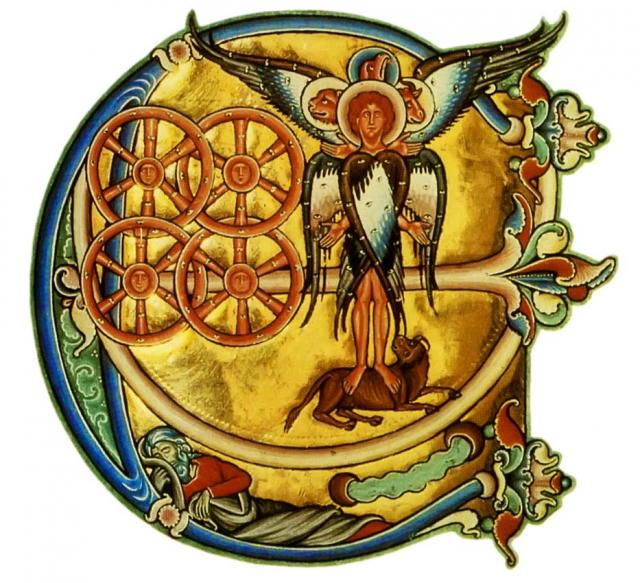
\includegraphics[width=0.8\textwidth]{ezechiel.jpg}\end{center}


\end{document}






